\documentclass{thesis}
% \usepackage[utf8]{inputenc}
\usepackage{csquotes}
\usepackage{enumitem}
\usepackage{blindtext}

% SIunitx formatting
% ------------------
\usepackage{siunitx}
\DeclareSIUnit\pixel{px}
\DeclareSIUnit\mag{X}
\DeclareSIUnit\NA{NA}
\DeclareSIUnit\hour{hr}
\DeclareSIUnit\molar{M}


% Biblatex formatting
% -------------------
\usepackage[
    backend=biber,
    style=numeric,
    refsection=chapter,
    sorting=none,
    maxcitenames=2,
    mincitenames=1,
]{biblatex}
\renewbibmacro{in:}{}  % https://tex.stackexchange.com/questions/10682/suppress-in-biblatex

% Add bibresources for biblatex
\addbibresource{chapter-1/chapter-1.bib}
\addbibresource{chapter-2/chapter-2.bib}
\addbibresource{chapter-3/chapter-3.bib}
\addbibresource{chapter-4/chapter-4.bib}
\addbibresource{chapter-5/chapter-5.bib}
\addbibresource{cppendix-A/appendix-A.bib}


% THE BEGINNING
% -------------
\begin{document}

% Some useful commands
\newcommand{\needref}{[\textit{\textcolor{orange}{references}}]}

% SI formatting options
\sisetup{
    range-phrase=--,
    range-units=single,
    per-mode=symbol,
    detect-all
}

% De good stuff
% -------------
\title{Pain and suffering in The Netherlands}
\author{Ryan}{Lane}
% \date{\today}

% De even better stuff
% --------------------
\frontmatter  % Roman numerals for early page numbers
% \section*{Propositions}

\begin{enumerate}
    \item Researchers conducting SEM-based backscattered electron imaging of biological tissue without the use of a negative potential bias are (literally) wasting time. \\
    \textit{This proposition pertains to this dissertation.}
    \item Integrated array tomography is the most viable solution for acquiring large-scale correlative light and electron microscopy datasets with sub-micron registration precision. \\
    \textit{This proposition pertains to this dissertation.}
    \item By mitigating nonspecific labeling artefacts and correcting for registration errors, neural networks trained on correlative light and electron microscopy data are capable of providing higher quality fluorescence information than fluorescence microscopes. \\
    \textit{This proposition pertains to this dissertation.}
    \item The future of correlative light and electron microscopy relies on improved protocols for sample preparation rather than instrumentation. \\
    \textit{This proposition pertains to this dissertation.}
    \item The next revolution in dense reconstruction of biological specimens will come from X-ray nano-tomography.
    \item By manufacturing women's clothing with impractical or nonexistent pockets, the fashion industry has exploited women into the purchasing of hand bags.
    \item If intelligent lifeforms existed elsewhere in our galaxy, we would be aware of them by now.
    \item Humanity and asteroids pose the two greatest existential threats to our planet; the best way to ensure the survival of our planet is therefore for all humans not contributing to an asteroid-detonation strategy to die.
    \item Art is not open to interpretation; it means precisely what the artist meant it to and nothing more.
    \item Inaccessibility of glass recycling facilities undermines the ``green" credentials of TU Delft.
    % \item A civilization is more likely to conquer its neighbor if it began food production first.
    % \item It is hypocritical of TU Delft to tout its green credentials whilst hiding the glass recycling in the basement of Building 22.
    % \item The key factor in the success of a city is a diversified labor market.
\end{enumerate}

\begin{titlepage}

\begin{center}

% Extra whitespace at the top.
\vspace*{2\bigskipamount}

% Print the title.
{\makeatletter
\titlestyle\bfseries\LARGE\@title
\makeatother}

% Print the optional subtitle.
{\makeatletter
\ifx\@subtitle\undefined\else
    \bigskip
    \titlefont\titleshape\Large\@subtitle
\fi
\makeatother}

\end{center}

\cleardoublepage
\thispagestyle{empty}

\begin{center}

% The following lines repeat the previous page exactly.

\vspace*{2\bigskipamount}

% Print the title.
{\makeatletter
\titlestyle\bfseries\LARGE\@title
\makeatother}

% Print the optional subtitle.
{\makeatletter
\ifx\@subtitle\undefined\else
    \bigskip
    \titlefont\titleshape\Large\@subtitle
\fi
\makeatother}

% Uncomment the following lines to insert a vertically centered picture into
% the title page.
%\vfill
%\includegraphics{title}
% \vfill

% Apart from the names and dates, the following text is dictated by the
% promotieregelement.

{\Large\titlefont\bfseries Proefschrift}

\bigskip
\bigskip

ter verkrijging van de graad van doctor

aan de Technische Universiteit Delft,

op gezag van de Rector Magnificus prof.~ir.~K.C.A.M.~Luyben,

voorzitter van het College voor Promoties,

in het openbaar te verdedigen op dinsdag 1 januari 2015 om 10:00 uur

\bigskip
\bigskip

door

\bigskip
\bigskip

% Print the full name of the author.
\makeatletter
{\Large\titlefont\bfseries\@firstname\ {\titleshape\@lastname}}
\makeatother

\bigskip
\bigskip

Fachlehrer für Mathematik und Physik, \\
Eidgenössische Polytechnische Schule, Zürich, Zwitserland,

geboren te Ulm, Duitsland.

% Extra whitespace at the bottom.
\vspace*{2\bigskipamount}

\end{center}

\clearpage
\thispagestyle{empty}

% The following line is dictated by the promotieregelement.
\noindent Dit proefschrift is goedgekeurd door de

% List the promotors (supervisors).
\medskip\noindent
\begin{tabular}{l}
    promotor: prof.\ dr.\ A.\ Kleiner \\
    copromotor: dr.\ A.A.\ Aaronson
\end{tabular}

\bigskip
\noindent Samenstelling promotiecommissie:

% List the committee members, starting with the Rector Magnificus and the
% promotor(s) and ending with the reserve members.
\medskip\noindent
\begin{tabular}{p{3cm}l}
    Rector Magnificus, & voorzitter \\
    Prof.\ dr.\ A.\ Kleiner, & Technische Universiteit Delft \\
    Dr.\ A.A.\ Aaronson, & Technische Universiteit Delft \\

    \medskip
    \mbox{\emph{Onafhankelijke leden:}} & \\

    Prof.\ dr.\ A.\ Jansen & Technische Universiteit Delft \\
    % Special case, only for very long names
    \mbox{Prof.\ dr.\ ir.\ A.B.C.D.\ van de Lange-Achternaam} & \\
      & Technische Universiteit Delft \\
    Prof.\.dr.\ N.\ Nescio & Politecnico di Milano, Itali\"e \\
    Prof.\ dr.\ ir.\ J.\ Doe, & Technische Universiteit Delft, reservelid \\

    \medskip
    \mbox{\emph{Overige leden:}} & \\
    Prof.\ dr.\ ir.\ J.\ de Wit, & Technische Universiteit Delft \\
    Dr.\ ir.\ Q.\ de Zwart, & Technische Universiteit Eindhoven \\
\end{tabular}

% Include the following disclaimer for committee members who have contributed
% to this dissertation. Its formulation is again dictated by the
% promotieregelement.
\medskip
\noindent Prof.\ dr.\ ir.\ J.\ de Wit heeft in belangrijke mate aan de totstandkoming van het proefschrift bijgedragen.

% % Here you can include the logos of any institute that contributed financially
% % to this dissertation.
% \vfill
% \begin{center}
%     
\includegraphics[height=0.5in]{title/logos/tudelft}
%     \hspace{2em}
%     \includegraphics[height=0.5in]{title/logos/casimir} \\
%     \includegraphics[height=0.5in]{title/logos/fom}
%     \hspace{2em}
%     
\includegraphics[height=0.5in]{title/logos/nwo}
% \end{center}
% \vfill

\noindent
\begin{tabular}{@{}p{0.2\textwidth}@{}p{0.8\textwidth}}
    \textit{Keywords:} & \ldots \\[\medskipamount]
    \textit{Printed by:} & Johannes Gutenberg \\[\medskipamount]
    \textit{Front \& Back:} & Beautiful cover art that captures the entire content of this thesis in a single illustration.
\end{tabular}

\vspace{4\bigskipamount}

\noindent Copyright \textcopyright\ 2015 by A.~Einstein


\medskip
\noindent ISBN 000-00-0000-000-0

\medskip
\noindent An electronic version of this dissertation is available at \\
\url{http://repository.tudelft.nl/}.

\end{titlepage}

\tableofcontents
\chapter*{Summary}
\addcontentsline{toc}{chapter}{Summary}
\setheader{Summary}

Summary in English. \blindtext

A new paragraph with a citation \cite{hildebrand2017whole}. Let us also add some numbers with units like \SI{100}{\milli\gram} and even a range of units \SIrange{14}{27}{\kilo\pascal}. \blindtext Could also look at units in math mode like $\SI{13.8}{\newton\per\metre}$. Let's follow this up with some math \cite{delpiano2018automated}.

\blindmathpaper


% De bestest stuff
% ----------------
\mainmatter  % switch to Arabic numerals for the page numbers
\chapter{Introduction}
\label{chap:1}
\begin{refsection}

% Sections
\section{Introduction}
\label{sec:4.1_intro}


% Motivate from EM perspective
% bio-insight from EM is hard
% CLEM has been developed to assist

Electron microscopy (EM) has transformed the way in which biologists understand intra- and inter-cellular systems. Due to the lack of inherent biological specificity, however, interpretation of EM datasets typically requires tedious expert analysis and annotation. For this reason, fluorescence microscopy (FM) is often used in conjunction with EM, complementing structural data with targeted biological labels. Fluorescent labelling, however, comes with several drawbacks. Sample preparation protocols are often laborious, time-consuming, and potentially damaging to the sample. Protocols must also be adapted to limit concentrations of heavy metal staining if intermediate processing of the sample is to be avoided \cite{kuipers2015scanning,lane2021optimization}. Fluorescent labelling is also susceptible to bleedthrough when multiple fluorophores are expressed in a single sample as well as varying specificity---Hoechst dyes, for instance, bind to both DNA and RNA. Furthermore, registering the separate imaging modalities across large spatial extents remains a technically challenging and primarily manual task \cite{russell20173d} [other references]. Correlative fluorescence and electron microscopy experiments are therefore typically limited in scope to the micron or tens of microns scale, and thus so are the regions for which biological labels can be provided \cite{russell20173d} [other references].

As recognition of organelles and other subcellular structures remains a pivotal obstacle in biological EM, we questioned whether large-scale EM datasets could be supplemented with biological labels through alternate means. To address this question, we sought to leverage recent advances in deep learning. Deep convolutional neural networks (CNN) in particular have been shown to be capable of inferring complex, non-linear relationships from image data \cite{he2016deep,januszewski2018high}. Prior work involving deep CNNs in the context of electron microscopy data has primarily been limited to applications in segmentation, denoising, and compressed sensing \cite{ede2021deep}. Semantic segmentation, the classification of pixels into discrete categories, does ultimately serve the purpose of adding biological labels to EM data. However, modern deep learning approaches require hours of tedious expert segmentation \cite{huang2014identifying,heinrich2018synaptic,liu2020automatic,spiers2021deep}. In order for \textcite{heinrich2020automatic} to amass sufficient training data for organelle segmentation, it required one person two weeks of manual segmentation per \SI{1}{\micro\meter^3} volume of image data; 28 blocks of this size were manually annotated in total to enable whole cell organelle segmentation.

Although relatively little attention has been paid to alternative applications in deep learning for EM data, recent work has focused on generating biological labels from other imaging modalities. \textcite{christiansen2018silico} designed a deep neural network to predict fluorescence labels from transmitted light images. \textcite{ounkomol2018label} extended the technique to generate 3D fluorescence from stacks of transmitted light microscopy data and further demonstrated the possibility of predicting immunofluorescence from EM images in order to facilitate automatic registration of fluorescence data with EM. To address the challenge of adding biological specificity to large-scale EM datasets, we thus explored the potential for a CNN to make label-free fluorescence predictions from electron microscopy image data.

In this work we present a deep CNN developed for generating fluorescence predictions on large-scale EM data of tissue and cellular samples. We demonstrate the performance of our model on thin sections of rat pancreas tissue, which have been immunolabelled with Alexa Fluor 594 and given a Hoechst counterstain, as well as Hoechst-stained sections of resin-embedded HeLa cells. Network predictions are quantitatively evaluated against corresponding true fluorescence images based on the Pearson correlation coefficient (PCC, or $\rho$) as well as by assessing human recognition of fluorescence predictions on cell nuclei. We additionally assess the network's robustness by measuring its predictive power on EM datasets acquired with varying imaging parameters. Finally, we explore the potential of correlative and predicted fluorescence signals for use as labels in segmentation experiments.






% \subsection{Things we will show}
% \begin{itemize}[noitemsep]
%     \item Can train a CNN to predict fluorescence based on registered CLEM images as training data
%     \begin{itemize}
%         \item Demonstrate on rat pancreas tissue: cell nuclei and insulin granules (micron scale and sub-diffraction limit)
%         \item Demonstrate on zebrafish: cell nuclei
%         \item Demonstrate on mouse heart tissue: phospholamban labelled with TRITC
%         \item Validate with PCC etc.\ and manual counting (for rat pancreas cell nuclei only)
%     \end{itemize}

%     \item CLEMnet is robust
%     \begin{itemize}
%         \item Predictions can be made on different rats
%         \item Predictions can be made on lower signal images (lower dwell) when trained with noise augmentation
%     \end{itemize}

%     \item CLEMnet predictions can be used for (semi/fully)-automated segmentation
%     \begin{itemize}
%         \item CLEMnet data slightly outperforms CLEM data for segmenting cell nuclei
%         \item Caveat that segmentation falls short of manual segmentation
%     \end{itemize}
% \end{itemize}




% Deep convolutional neural networks (CNN) are capable of inferring complex, non-linear relationships between images. Prior work applying deep learning strategies to EM data has often revolved around segmentation tasks. Competitions such as the IEEE International Symposium on Biomedical Imaging (ISBI) challenge for segmentation of neuronal structures in electron microscopic stacks \cite{arganda2015crowdsourcing} have inspired generations of neural network architecture development such as the U-net \cite{ronneberger2015u} and its 3D counterpart \cite{cciccek20163d}. More recently, a CNN has been employed for for whole cell organelle segmentation in a micron-sized volumetric EM dataset \cite{heinrich2020automatic}. Relatively little attention has been paid to alternative applications of deep learning algorithms for volumetric EM data. \textcite{ounkomol2018label} trained a model to facilitate automatic registration of multichannel fluorescence data to EM array tomography data. % Limited to myelin. [More examples].




% As recognition of organelles and other subcellular structures remains a pivotal obstacle in biological EM, [lots and lots of work] has centered around segmentation and classification of these structures. More recently, these efforts have focused on employing deep learning strategies to infer [descriptive adjective] patterns from EM image data rich in structural information \cite{heinrich2020automatic} [25 references therein]. [only expert-level people would otherwise be capable of discerning].
% %
% Competitions such as the IEEE International Symposium on Biomedical Imaging (ISBI) challenge for segmentation of neuronal structures in electron microscopic stacks \cite{arganda2015crowdsourcing} have inspired generations of neural network architecture development such as the U-net \cite{ronneberger2015u} and its 3D counterpart \cite{cciccek20163d}. More recently, a CNN has been employed for whole cell organelle segmentation in a micron-sized volumetric EM dataset \cite{heinrich2020automatic}.


% %
% [No one(?) is making use of multimodal datasets to assist in recognition and segmentation of EM datasets]. 




% References
\printbibliography[title={References}]
\end{refsection}
  % intro
% \chapter[Optimization of negative stage bias potential]{Optimization of negative stage bias potential for faster imaging in large-scale electron microscopy}
\label{chap:2}
\begin{refsection}

% Abstract
\section*{Abstract}
\begin{small}
    Large-scale electron microscopy (EM) allows analysis of both tissues and macromolecules in a semi-automated manner, but acquisition rate forms a bottleneck. We reasoned that a negative bias potential may be used to enhance signal collection, allowing shorter dwell times and thus increasing imaging speed. Negative bias potential has previously been used to tune penetration depth in block-face imaging. However, optimization of negative bias potential for application in thin section imaging will be needed prior to routine use and application in large-scale EM. Here, we present negative bias potential optimized through a combination of simulations and empirical measurements. We find that the use of a negative bias potential generally results in improvement of image quality and signal-to-noise ratio (SNR). The extent of these improvements depends on the presence and strength of a magnetic immersion field. Maintaining other imaging conditions and aiming for the same image quality and SNR, the use of a negative stage bias can allow for a 20-fold decrease in dwell time, thus reducing the time for a week long acquisition to less than \SI{8}{\hour}. We further show that negative bias potential can be applied in an integrated correlative light electron microscopy (CLEM) application, allowing fast acquisition of a high precision overlaid LM-EM dataset. Application of negative stage bias potential will thus help to solve the current bottleneck of image acquisition of large fields of view at high resolution in large-scale microscopy.
\end{small}

\clearpage

\section{Introduction}
\label{sec:4.1_intro}


% Motivate from EM perspective
% bio-insight from EM is hard
% CLEM has been developed to assist

Electron microscopy (EM) has transformed the way in which biologists understand intra- and inter-cellular systems. Due to the lack of inherent biological specificity, however, interpretation of EM datasets typically requires tedious expert analysis and annotation. For this reason, fluorescence microscopy (FM) is often used in conjunction with EM, complementing structural data with targeted biological labels. Fluorescent labelling, however, comes with several drawbacks. Sample preparation protocols are often laborious, time-consuming, and potentially damaging to the sample. Protocols must also be adapted to limit concentrations of heavy metal staining if intermediate processing of the sample is to be avoided \cite{kuipers2015scanning,lane2021optimization}. Fluorescent labelling is also susceptible to bleedthrough when multiple fluorophores are expressed in a single sample as well as varying specificity---Hoechst dyes, for instance, bind to both DNA and RNA. Furthermore, registering the separate imaging modalities across large spatial extents remains a technically challenging and primarily manual task \cite{russell20173d} [other references]. Correlative fluorescence and electron microscopy experiments are therefore typically limited in scope to the micron or tens of microns scale, and thus so are the regions for which biological labels can be provided \cite{russell20173d} [other references].

As recognition of organelles and other subcellular structures remains a pivotal obstacle in biological EM, we questioned whether large-scale EM datasets could be supplemented with biological labels through alternate means. To address this question, we sought to leverage recent advances in deep learning. Deep convolutional neural networks (CNN) in particular have been shown to be capable of inferring complex, non-linear relationships from image data \cite{he2016deep,januszewski2018high}. Prior work involving deep CNNs in the context of electron microscopy data has primarily been limited to applications in segmentation, denoising, and compressed sensing \cite{ede2021deep}. Semantic segmentation, the classification of pixels into discrete categories, does ultimately serve the purpose of adding biological labels to EM data. However, modern deep learning approaches require hours of tedious expert segmentation \cite{huang2014identifying,heinrich2018synaptic,liu2020automatic,spiers2021deep}. In order for \textcite{heinrich2020automatic} to amass sufficient training data for organelle segmentation, it required one person two weeks of manual segmentation per \SI{1}{\micro\meter^3} volume of image data; 28 blocks of this size were manually annotated in total to enable whole cell organelle segmentation.

Although relatively little attention has been paid to alternative applications in deep learning for EM data, recent work has focused on generating biological labels from other imaging modalities. \textcite{christiansen2018silico} designed a deep neural network to predict fluorescence labels from transmitted light images. \textcite{ounkomol2018label} extended the technique to generate 3D fluorescence from stacks of transmitted light microscopy data and further demonstrated the possibility of predicting immunofluorescence from EM images in order to facilitate automatic registration of fluorescence data with EM. To address the challenge of adding biological specificity to large-scale EM datasets, we thus explored the potential for a CNN to make label-free fluorescence predictions from electron microscopy image data.

In this work we present a deep CNN developed for generating fluorescence predictions on large-scale EM data of tissue and cellular samples. We demonstrate the performance of our model on thin sections of rat pancreas tissue, which have been immunolabelled with Alexa Fluor 594 and given a Hoechst counterstain, as well as Hoechst-stained sections of resin-embedded HeLa cells. Network predictions are quantitatively evaluated against corresponding true fluorescence images based on the Pearson correlation coefficient (PCC, or $\rho$) as well as by assessing human recognition of fluorescence predictions on cell nuclei. We additionally assess the network's robustness by measuring its predictive power on EM datasets acquired with varying imaging parameters. Finally, we explore the potential of correlative and predicted fluorescence signals for use as labels in segmentation experiments.






% \subsection{Things we will show}
% \begin{itemize}[noitemsep]
%     \item Can train a CNN to predict fluorescence based on registered CLEM images as training data
%     \begin{itemize}
%         \item Demonstrate on rat pancreas tissue: cell nuclei and insulin granules (micron scale and sub-diffraction limit)
%         \item Demonstrate on zebrafish: cell nuclei
%         \item Demonstrate on mouse heart tissue: phospholamban labelled with TRITC
%         \item Validate with PCC etc.\ and manual counting (for rat pancreas cell nuclei only)
%     \end{itemize}

%     \item CLEMnet is robust
%     \begin{itemize}
%         \item Predictions can be made on different rats
%         \item Predictions can be made on lower signal images (lower dwell) when trained with noise augmentation
%     \end{itemize}

%     \item CLEMnet predictions can be used for (semi/fully)-automated segmentation
%     \begin{itemize}
%         \item CLEMnet data slightly outperforms CLEM data for segmenting cell nuclei
%         \item Caveat that segmentation falls short of manual segmentation
%     \end{itemize}
% \end{itemize}




% Deep convolutional neural networks (CNN) are capable of inferring complex, non-linear relationships between images. Prior work applying deep learning strategies to EM data has often revolved around segmentation tasks. Competitions such as the IEEE International Symposium on Biomedical Imaging (ISBI) challenge for segmentation of neuronal structures in electron microscopic stacks \cite{arganda2015crowdsourcing} have inspired generations of neural network architecture development such as the U-net \cite{ronneberger2015u} and its 3D counterpart \cite{cciccek20163d}. More recently, a CNN has been employed for for whole cell organelle segmentation in a micron-sized volumetric EM dataset \cite{heinrich2020automatic}. Relatively little attention has been paid to alternative applications of deep learning algorithms for volumetric EM data. \textcite{ounkomol2018label} trained a model to facilitate automatic registration of multichannel fluorescence data to EM array tomography data. % Limited to myelin. [More examples].




% As recognition of organelles and other subcellular structures remains a pivotal obstacle in biological EM, [lots and lots of work] has centered around segmentation and classification of these structures. More recently, these efforts have focused on employing deep learning strategies to infer [descriptive adjective] patterns from EM image data rich in structural information \cite{heinrich2020automatic} [25 references therein]. [only expert-level people would otherwise be capable of discerning].
% %
% Competitions such as the IEEE International Symposium on Biomedical Imaging (ISBI) challenge for segmentation of neuronal structures in electron microscopic stacks \cite{arganda2015crowdsourcing} have inspired generations of neural network architecture development such as the U-net \cite{ronneberger2015u} and its 3D counterpart \cite{cciccek20163d}. More recently, a CNN has been employed for whole cell organelle segmentation in a micron-sized volumetric EM dataset \cite{heinrich2020automatic}.


% %
% [No one(?) is making use of multimodal datasets to assist in recognition and segmentation of EM datasets]. 



\section{Results}
\label{sec:2.2_results}

% 2.2.1
% -----
\subsection{Negative bias potential enhances signal in routine EM samples}

We first illustrate how the use of a potential bias can improve signal collection in a typical SEM experiment. A potential bias of \SI{-1}{\kilo\volt} is applied to the stage of an SEM with an integrated fluorescence microscope (Figure \ref{fig:2.1_setup}A \& B). The bias is applied via an external power supply connected to a custom stage plate such that the sample is electrically isolated from the rest of the fluorescence microscope and electrical components of the stage \cite{vos2021retarding}. By generating an electric field between the sample and the BSE detector, the bias potential accelerates signal electrons inwards away from their otherwise linear trajectories. Because of their lower energy, secondary electrons (<\,\SI{50}{\electronvolt}) are redirected inside the inner annulus of the BSE detector, while higher energy backscattered electrons (>\,\SI{50}{\electronvolt}) are redirected over a wider area depending on their initial emission angle and energy.

Pancreas tissue was prepared for integrated fluorescence-electron microscopy as described in Section \ref{sec:2.4.2_sampleprep}. No post-staining was applied resulting in lower contrast relative to other EM sample preparation protocols \cite{kuipers2015scanning}. EM images of EPON-embedded, \SI{80}{\nano\meter} tissue were acquired in immersion mode with and without a \SI{-1}{\kilo\volt} bias potential (Figure \ref{fig:2.1_setup}A \& B). When subject to a bias potential, EM images demonstrate noticeably higher contrast and less noise (Figure \ref{fig:2.1_setup}C \& G). The primary beam energy was increased by \SI{1}{\kilo\volt} such that the landing energy was held constant at \SI{1.5}{\kilo\electronvolt} in accordance with the section thickness. Data acquired with increased primary energy but without the use of stage bias (Figure \ref{fig:2.1_setup}D) reveals that the increase in apparent signal does not arrive solely from an increased primary energy. Moreover, the importance of maintaining a sufficiently low landing energy becomes clear by the visible artefacts from the ITO-coated glass substrate that appear with higher energies. The \SI{0.4}{\nano\ampere} beam current and \SI{5}{\micro\second\per\pixel} dwell time are held constant in each acquisition. The gain of the BSE detector had to be decreased while applying the negative bias to prevent the detector from saturating.

% Figure 2.1 (setup)
% -----------------
\begin{figure}[!tb]
    \centering
    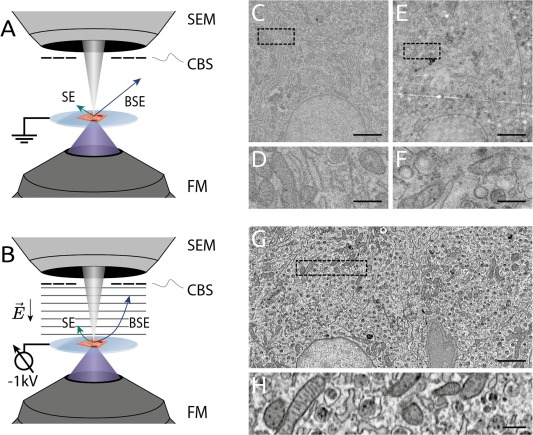
\includegraphics[width=\linewidth]{chapter-2/figures_JPEG_LQ/fig2-1_setup.jpg}
    \caption{Negative bias potential significantly enhances EM contrast in tissue. Schematic of integrated microscope without (A) and with (B) an applied stage bias. Electric field induced by the bias potential accelerates electrons emitted from the sample to the CBS detector. EM images of rat pancreas tissue without (C -- F) and with (G \& inset H) the use of stage bias. Biased images (G \& inset H) were acquired at \SI{2.5}{\kilo\electronvolt} primary energy with a \SI{-1}{\kilo\volt} bias potential---hence, a \SI{1.5}{\kilo\electronvolt} landing energy. For the sake of comparison, unbiased images (C \& inset D) were acquired with the same landing energy, while unbiased images (E \& inset F) were acquired with the same primary energy. The per-pixel dwell is held constant across all images at \SI{5}{\micro\second}. Vast improvement in EM signal and contrast can be seen by comparing insets (D \& F) with (H). Scale bars: \SI{2}{\micro\meter} (C, E, \& G); \SI{0.5}{\micro\meter} (D, F, \& H). Raw data at full resolution is available at \href{www.nanotomy.org}{Nanotomy}.}
    \label{fig:2.1_setup}
\end{figure}


% 2.2.2
% -----
\subsection{Simulating signal electron trajectories with and without negative potential bias}

% Figure 2.2 (simulations)
% ------------------------
\begin{figure}[!tb]
    \centering
    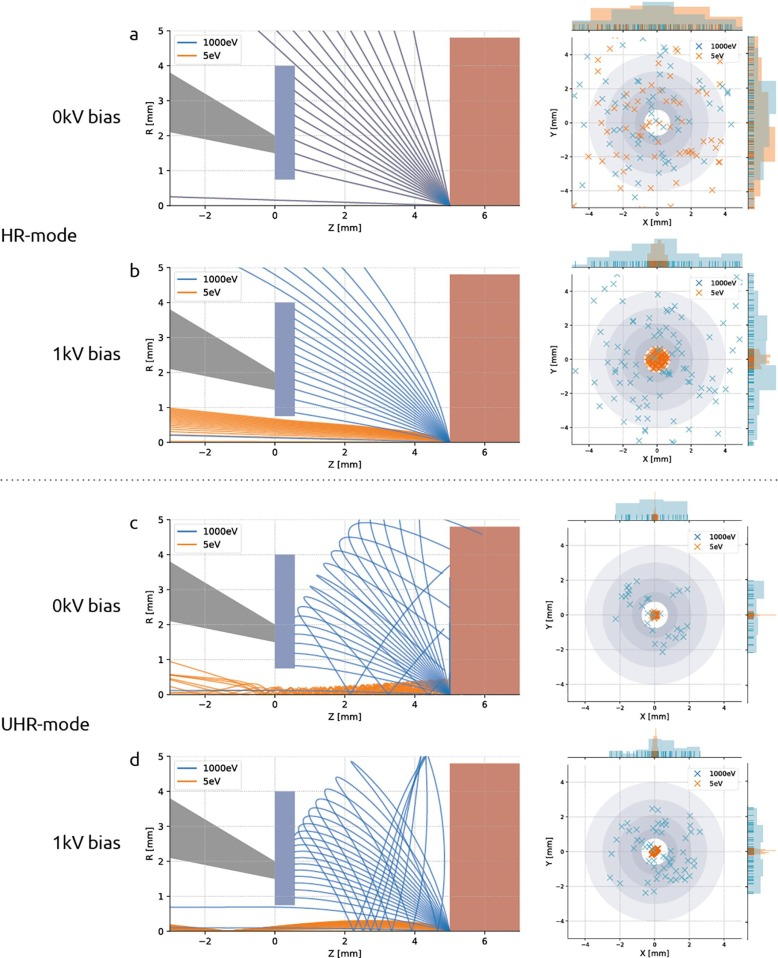
\includegraphics[width=0.85\linewidth]{chapter-2/figures_JPEG_LQ/fig2-2_simulations.jpg}
    \caption{Signal electron trajectories demonstrate the efficacy of stage bias in redirecting BSEs to the detector while simultaneously filtering out secondary electrons. Trajectory plots for SE and BSE bundles launched from the sample plane (left) and scatter plots (right) show the spatial distribution of signal electrons at the detector plane. In HR-mode, SEs and BSEs travel in overlapping, linear paths without the presence of an electric field (A), but BSEs get accelerated towards the detector when a negative bias potential is introduced (B). Signal electrons take on spiral trajectories in the presence of an immersion magnetic field (C), but are again steered to the detector when an electric field is added (D). In each set of simulations, BSEs (blue) and SEs (orange) are launched from the sample plane at $z =$ \SI{5}{\milli\meter}. Trajectory plots show geometry of the pole piece (grey), CBS detector (blue), and stage plate (red). Scatter plots show $x, y$ coordinates of signal electrons at the detector plane ($z =$ \SI{5}{\milli\meter}). Spatial distributions of signal electrons are plotted on the margins of the scatter plots.}
    \label{fig:2.2_simulations}
\end{figure}

Electron trajectories were simulated to better ascertain how a negative bias potential may give rise to better signal detection. Secondary electron and backscattered electron (BSE) trajectories were simulated for a variety of EM imaging conditions (Figure \ref{fig:2.2_simulations}). A model of the optical layout within the integrated microscope was developed in Electron Optical Design (EOD) \cite{lencova2008new} incorporating the geometry of the Verios 460 SEM objective lens and concentric backscatter (CBS) detector. The negative potential bias is factored into the model by implementing the sample plane as an additional lens element, which can then be biased to an arbitrary voltage. To mirror the \SI{5}{\milli\meter} working distance of our microscope, the end of the pole piece (grey element in Figure \ref{fig:2.2_simulations}) and start of the sample plane (red) are situated at $z=$ \SI{0}{\milli\meter} and $z=$ \SI{5}{\milli\meter} respectively. The roughly \SI{0.5}{\milli\meter} thick CBS detector (blue) is then located immediately below the pole piece.

Simulations were done for both non-immersion (high resolution or HR) and immersion (ultra-high resolution or UHR) SEM operation modes. For the case of non-immersion mode (Figure \ref{fig:2.2_simulations}A \& B), the magnetic focusing field is contained within the objective lens and therefore does not play a role in the signal electron trajectories. In these instances, the trajectories of the SEs and BSEs are dictated entirely by their initial velocity and the electric field due to the bias potential. In UHR-mode (Figure \ref{fig:2.2_simulations}C \& D), however, the sample is immersed in a strong magnetic field that both focuses the primary beam and---together with the electric field---alters the paths taken by the signal electrons. For this reason, the magnetic field strength is calculated by the field strength required to focus a parallel beam propagating in the $+z$ direction at the sample plane.

For each scenario shown, a bundle of secondary ($E_0 =$ \SI{5}{\electronvolt}) and backscattered electrons ($E_0 =$ \SI{1}{\kilo\electronvolt}) is emitted from the origin at $z =$ \SI{5}{\milli\meter}. The angular distribution is given by Lambert's cosine distribution \cite{reimer1998emission}. A screen is placed at the detector plane to record the radial position of the signal electrons, from which the scatter plots are generated (Figure \ref{fig:2.2_simulations}). The grey rings of varying diameter represent the individual segments of the CBS detector. For the case of non-immersion mode and no potential bias (Figure \ref{fig:2.2_simulations}A), the region between the detector and sample planes is field-free and the signal electrons travel freely in straight paths coinciding with one another. Only when a bias potential is added (Figure \ref{fig:2.2_simulations}B) do the higher energy BSEs diverge from the secondaries, which, due to their low initial energy, are accelerated inside the BSE detector before they are able to spread out radially. The trajectories change when under the influence of a magnetic immersion field (Figure \ref{fig:2.2_simulations}C) in which case the Lorentz force causes the signal electrons to spiral about the optical axis \cite{mullerova2009collection}. The low energy SEs remain tightly coiled as they propagate up through the BSE detector while the higher energy BSEs stretch out over greater radial distances. Whether the BSEs collide into the detector depends largely on the emission angle. The addition of a \SI{1}{\kilo\volt} bias potential (Figure \ref{fig:2.2_simulations}D) enables BSEs with a wider distribution of emission angles to reach the detector, resulting in the collection of more signal. These results suggest no secondary electron is ever registered as a count by the BSE detector---either because it is accelerated inside the detector or (in the field-free case) because it is of too little energy to generate an electron-hole pair \cite{vsakic2011boron}.

The collection efficiency of BSEs increases monotonically with increasing negative bias potential for both imaging modes (Figure \ref{fig:2.S1_percentages}). These results agree with what is suggested by the trajectory plots of Figure \ref{fig:2.2_simulations}---that the electric field generated by the stage bias tapers the radial spread of the BSEs leading to a greater percentage of BSEs collected. Note that the percentage of BSEs detected is greater for HR-mode across the range of bias potentials simulated. It therefore seems advantageous to prefer non-immersion mode, however, greater collection efficiency is only one factor to consider. The magnetic immersion field results in lower aberrations, meaning that for high resolution imaging, UHR mode is still often favourable. While the geometry modelled here is specific to our particular electron microscope, simulations were extended over a range of working distances and were found to follow the same general trends.% The electron trajectory data included in the supplemental data allows a user to input a range of working distances to simulate what BSE collection efficiency they might experience with their setup. Table \ref{} lists the available parameter space in which it is possible to trace BSE trajectories. Code for calculating the radial position of individual BSEs at a given detector plane is available within the supplemental material (Appendix \ref{}).


% 2.2.3
% -----
\subsection{Experimental optimization of negative potential bias leads to increased throughput}

EM imaging was expanded to encompass a wider imaging parameter space across a sequence of dwell times and negative bias potentials for both immersion and non-immersion mode based on the simulations (Figure \ref{fig:2.3_matrices}). The primary beam energy was increased together with the bias potential to hold the landing energy constant at \SI{1.5}{\kilo\electronvolt}. Likewise, the gain of the CBS detector was adjusted with each bias potential to keep the intensity levels from clipping. The detector gain and offset were manually calibrated to acquire over the full 16-bit range of the detector. This was not always possible, however, as many of the images acquired with low or no bias potential took up only a fraction of the detector's bandwidth, even at maximum gain.

% Figure 2.3 (matrices)
% ---------------------
\begin{figure}[!tb]
    \centering
    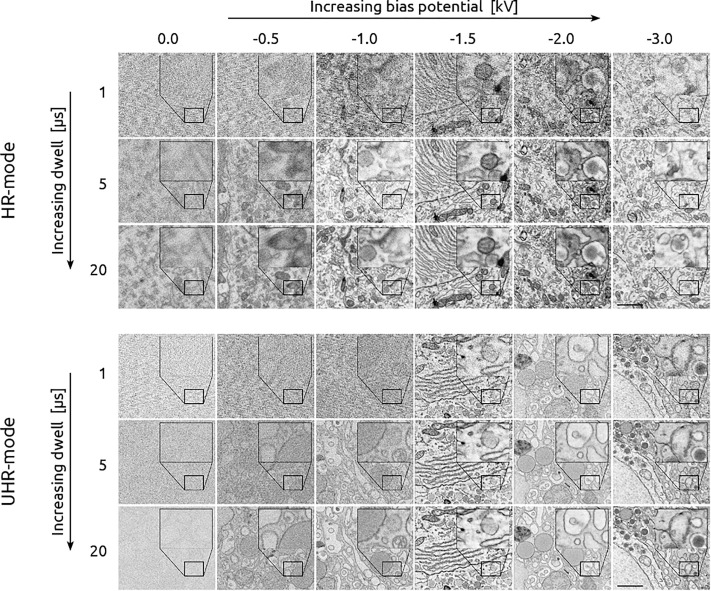
\includegraphics[width=\linewidth]{chapter-2/figures_JPEG_LQ/fig2-3_matrices.jpg}
    \caption{Negative bias potential delivers 5--20 times faster imaging while maintaining image quality. Bias potential varies from \SIrange[range-phrase=\text{ to }]{0}{-3}{\kilo\volt} (left to right) while the integration time varies from \SIrange[range-phrase=\text{ to }]{1}{20}{\micro\second} (top to bottom) for both the non-immersion (top) and immersion mode (bottom) image matrices. All images acquired with \SI{1.5}{\kilo\electronvolt} landing energy to match penetration depth. Scale bars: \SI{1}{\micro\meter}. Raw data is available at \href{www.nanotomy.org}{Nanotomy}.}
    \label{fig:2.3_matrices}
\end{figure}

An increase in image signal with increasing negative bias potential for both imaging modes up to roughly \SI{-1500}{\volt} was recorded (Figure \ref{fig:2.3_matrices}), after which it becomes difficult to perceive notable differences in image quality. The signal appears to improve more gradually in non-immersion mode, whereas the improvement for immersion mode is more abrupt. Furthermore, in certain instances, increasing the integration time by several factors results in a less substantial increase to the apparent SNR than a \SI{500}{\volt} increase to the negative bias potential. This is significant as the integration time is typically the primary imaging parameter to improve image quality—and large increases come at the direct expense of throughput.

Quantitative SNR measurements, based on the spectral signal-to-noise ratio (SSNR) \cite{unser1987new}, were made on the collection of images and averaged for each combination of bias potential, dwell, and imaging mode (Figure \ref{fig:2.4_snr}). These measurements were corroborated using a separate cross-correlation-based SNR method \cite{joy2002smart} (Figure \ref{fig:2.S2_comparison}). In particular, these measurements reveal that an image acquired in non-immersion mode with a \SI{1}{\micro\second} dwell time and \SI{-1.5}{\kilo\volt} bias potential yields roughly the same SNR as an image acquired with a \SI{5}{\micro\second} dwell but with no applied bias. The effect of the potential bias is even more pronounced in immersion mode where the SNR of a \SI{1}{\micro\second} image with a \SI{1.5}{\kilo\volt} stage bias exceeds that of a \SI{20}{\micro\second} image acquired without a bias. Fourier analysis was done to analyse the effect of the bias potential in different frequency domains (Figure \ref{fig:2.5_noise}). The center spot of the 2D FFTs—containing most of the signal—becomes more prominent with increasing bias potential. This growth is reflected in the SSNR spectra, which show order of magnitude increases in amplitude in the low spatial frequency domain. Furthermore, the high frequency streak artefacts present in the lower bias potential images---visible in the 2D FFTs---become suppressed at higher bias potentials.

% Figure 2.4 (SNR)
% ----------------
\begin{figure}[!tb]
    \centering
    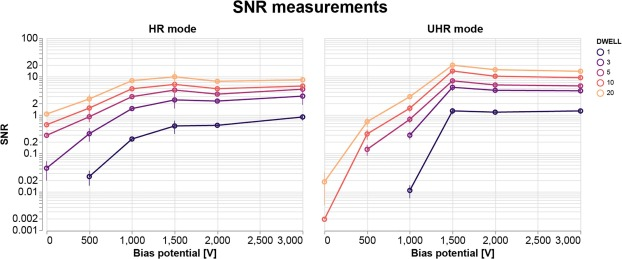
\includegraphics[width=\linewidth]{chapter-2/figures_JPEG_LQ/fig2-4_snr.jpg}
    \caption{Optimization of bias potential delivers SNR increases of multiple orders of magnitude. At bias potentials greater than \SI{1.5}{\kilo\volt}, the SNR is found to level off for both imaging modes. Images are comprised of varying stage bias potentials, integration times, and imaging modes but with fixed \SI{1.5}{\kilo\electronvolt} landing energy and \SI{5}{\milli\meter} working distance. Different color lines represent different dwell times as indicated by the legend. SNR measurements are averaged over five EM images at different areas of the tissue for each combination of bias potential, dwell time, and imaging mode. Error bars indicate the standard deviation in the SNR over the five images. Missing data points indicate a negative SNR, which may occur for images with extremely high noise.}
    \label{fig:2.4_snr}
\end{figure}


% Figure 2.5 (noise)
% ------------------
\begin{figure}[!tb]
    \centering
    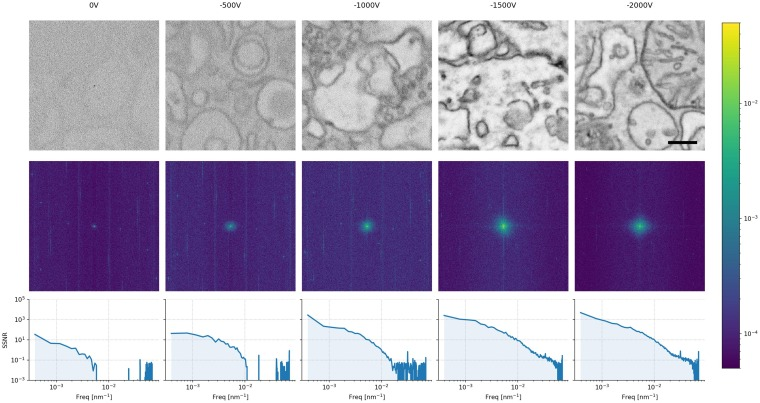
\includegraphics[width=\linewidth]{chapter-2/figures_JPEG_LQ/fig2-5_noise.jpg}
    \caption{Noise contributions suspected to originate from the scanning electronics are suppressed with increasing bias potential. Top: sequence of \SI{5}{\micro\second} dwell tissue images acquired in immersion mode with varying amounts of stage bias. Center: 2D FFTs of tissue images showing the central spot, which represents most of the signal, becoming more prominent with increasing bias potential up to \SI{-1.5}{\kilo\volt}. The 2D FFTs exhibit noticeable streak artefacts at higher frequencies, particularly in the lower bias potential images. We attribute these streaks to electric interference from the scanning electronics. Furthermore, there is a constant offset, which is likely a combination of shot noise from various sources, and may also include a component from the scanning electronics. Bottom: SSNR spectra show a division between the low frequency (primarily signal) and high frequency (primarily noise) portions of the tissue images. As the suspected scanning electronics noise is drowned out, the SNR improves dramatically. Scale bar: \SI{500}{\nano\meter}.}
    \label{fig:2.5_noise}
\end{figure}


% 2.2.4
% -----
\subsection{Potential bias allows for higher throughput EM and CLEM acquisitions}

Only small regions of interest are typically recorded at high resolution EM given that full section imaging at sub-\SI{10}{\nano\meter} resolution often takes an excessive amount of time. As a result of the enhanced signal-to-noise ratio afforded to us by the use of a negative bias potential, we are able to significantly expedite the imaging of a thin section of HeLa cells at \SI{5}{\nano\meter} resolution (Figure \ref{fig:2.6_cells}). Based on our empirical results (Figure \ref{fig:2.4_snr}), a negative potential bias of \SI{-1.5}{\kilo\volt} was chosen for EM imaging in immersion mode. A per-pixel dwell time of \SI{2}{\micro\second} was chosen to balance high SNR and image clarity with overall imaging time. Control images of the same cell were acquired without the use of a bias potential at the same landing energy (Figure \ref{fig:2.6_cells}A) and primary energy (Figure \ref{fig:2.6_cells}B). The total imaging time for this \SI{550}{\micro\meter} $\times$ \SI{350}{\micro\meter} area was \SI{5.6}{\hour}.

% Figure 2.6 (cells)
% ------------------
\begin{figure}[!tb]
    \centering
    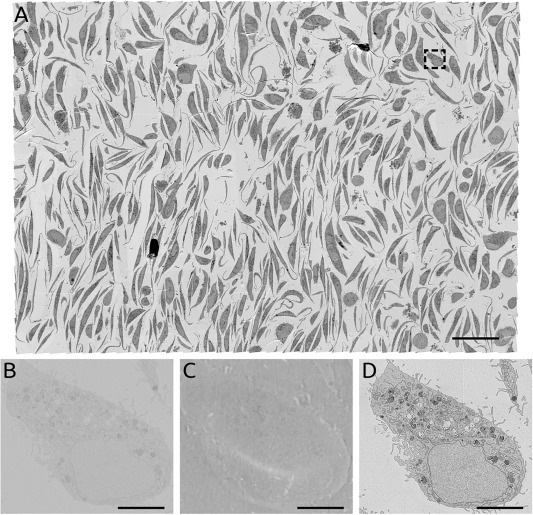
\includegraphics[width=\linewidth]{chapter-2/figures_JPEG_LQ/fig2-6_cells.jpg}
    \caption{Fast, high resolution EM gigapixel image of cultured cells. (A) EM acquisition of a \SI{100}{\nano\meter} section of HeLa cells as a nanotomy map. Section imaged at \SI{1.5}{\kilo\electronvolt} LE and with a \SI{-1.5}{\kilo\volt} bias potential. For the sake of comparison, one HeLa cell was acquired at multiple energy settings: (B) \SI{1.5}{\kilo\electronvolt} LE with no bias potential; (C) \SI{3}{\kilo\electronvolt} LE with no bias potential; (D) \SI{1.5}{\kilo\electronvolt} LE with \SI{-1.5}{\kilo\volt} bias potential—identical to that of the large-scale acquisition. Scale bars: \SI{50}{\micro\meter} (A); \SI{5}{\micro\meter} (B, C, \& D). Raw data is available for viewing via \href{www.nanotomy.org}{Nanotomy}.}
    \label{fig:2.6_cells}
\end{figure}

To demonstrate the application of a negative bias potential on samples also prepared for immunofluorescence, a large-scale acquisition was conducted on a section of rat pancreas tissue (Figure \ref{fig:2.7_rat}). Full section (\SI{0.5}{\milli\meter^2}) acquisition including fluorescence imaging, stage translations, and additional overhead factors was completed in \SI{8}{\hour}. Table \ref{tab:2.1_timing} provides an overview of the time spent on each aspect of the workflow, and exemplifies the potential time savings afforded by using a bias potential. We note that no post-staining was applied to this section in order to allow integrated acquisition of fluorescence for high-precision overlaid FM. Fluorescence images were acquired prior to EM to prevent quenching of the fluorescence due to electron beam irradiation. The insulin-producing beta cells---clustered within the islet of Langerhans---were immunolabelled and given a Hoechst counterstain to target cell nuclei as well as the rough endoplasmic reticulum in the exocrine region of the tissue (blue) (Figure \ref{fig:2.7_rat}A). The section edges can easily be discerned from the FM images, facilitating the area selection for subsequent EM imaging (Figure \ref{fig:2.7_rat}B). Here the islet (light grey region) can be seen surrounded by the exocrine tissue (dark grey). An automated registration procedure \cite{haring2017automated} was done to overlay the fluorescence signal onto the EM images (Figure \ref{fig:2.7_rat}C) such that the fluorescence signal is correlated at high resolution across the entire EM field of view (Figure \ref{fig:2.7_rat}D \& E). Additional details of how the correlative acquisition and reconstruction were done are provided in Sections \ref{sec:2.4.4_workflow} and \ref{sec:2.4.5_reconstruction} respectively.

% Figure 2.7 (rat)
% ----------------
\begin{figure}[!tb]
    \centering
    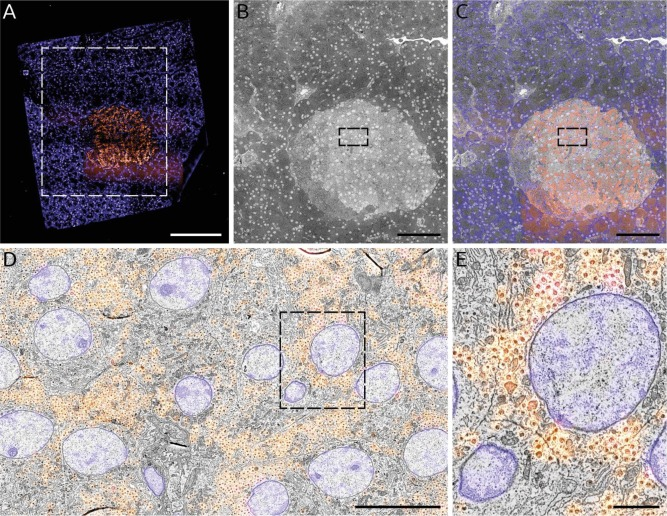
\includegraphics[width=\linewidth]{chapter-2/figures_JPEG_LQ/fig2-7_rat.jpg}
    \caption{Fast, correlative imaging of a complete EM section at high resolution. \SI{80}{\nano\meter} rat pancreas tissue was imaged at \SI{3}{\kilo\electronvolt} beam energy with a \SI{-1.5}{\kilo\volt} stage bias (\SI{1.5}{\kilo\electronvolt} landing energy) with \SI{2}{\micro\second} dwell as a nanotomy map. (A) Composite two-channel FM image of the tissue section: cell nuclei (blue) stained by Hoechst; insulin-producing beta cells (orange) immunolabeled with Alexa 594. (B) Composite EM image of the area outlined in (A) comprising the islet of Langerhans identified via FM imaging. (C) Correlative overlay of the islet and surrounding exocrine tissue. (D) Zoomed-in area of islet outlined in (B \& C) with inset (E) exhibiting the native resolution (\SI{5}{\nano\meter} pixel size) that exists across the entirety of the nanotomy map. Total imaging time is \SI{8}{\hour}, the majority of which is taken up by the high-resolution EM imaging. Note that a similar area at this pixel size (see e.g. \textcite{ravelli2013destruction}) typically takes upwards of \SI{24}{\hour} with TEM. Scale bars: \SI{200}{\micro\meter} (A); \SI{100}{\micro\meter} (B \& C); \SI{10}{\micro\meter} (D); \SI{2}{\micro\meter} (E). Raw data is available via \href{www.nanotomy.org}{Nanotomy}.}
    \label{fig:2.7_rat}
\end{figure}


% Table 2.1 (timing)
% ------------------
\begin{table}[!tb]
    \centering
    \caption{Use of optimized potential bias leads to an 80\% reduction in total imaging time for a typical large-scale acquisition. The total imaging time is highly dependent on the ROI size, which may vary widely depending on the biological application. Here the typical diameter of an islet of Langerhans is given, while in Figure \ref{fig:2.7_rat} a \SI{700}{\micro\meter} $\times$ \SI{700}{\micro\meter} area was chosen as the ROI—resulting in the \SI{8}{\hour} total acquisition time. Total imaging times for arbitrary ROI sizes can be determined by first calculating the number of image tiles needed: $N=\text{ceil}\left((L-ow) - (w-ow)\right)^2$ where $L$ is the typical section or ROI width, $o$ is the percentage overlap between image tiles, and $w$ is the field of view. Note that the negative overlap given for the low-magnification CLEM tiles reflects that these tiles do not overlap with one another.}
    \footnotesize
    \begin{tabular}{@{}p{15mm}p{30mm}rrrr@{}}
    \toprule
    \multicolumn{1}{r}{} & \multicolumn{1}{r}{} & \multicolumn{2}{c}{\textbf{Low-mag CLEM}} & \multicolumn{2}{c}{\textbf{Hi-mag EM}} \\
     \arrayrulecolor{black!30}\cmidrule(l){3-4} \cmidrule(l){5-6}
     &  & \textbf{No bias} & \textbf{Bias} & \textbf{No bias} & \textbf{Bias} \\
     \arrayrulecolor{black!30}\midrule
     & Pixel size & 36.6 nm &  & 4.88 nm &  \\
     & Dwell & 10 µs & 2 µs & 10 µs & 2 µs \\
     & Field of View & 150 µm &  & 20 µm &  \\
     & Overlap (b/w images) & −36 µm (−24\%) &  & 2.4 µm (12\%) &  \\
     & N. pixels & 16.8 Mpx &  & 16.8 Mpx &  \\
    \multirow{-6}{*}{EM} & Acquisition time & 168 s & 33.6 s & 168 s & 33.6 s \\
    \arrayrulecolor{black!30}\midrule
     & Exposure time & 5 s &  &  &  \\
     & N. channels & 2 &  &  &  \\
    \multirow{-3}{*}{FM} & Acquisition time & 10 s &  &  &  \\
    \arrayrulecolor{black!30}\midrule
     & Registration procedure & 20 s &  &  &  \\
    \multirow{-2}{*}{Overhead} & Stage translation & 4 s &  & 2 s &  \\
    \arrayrulecolor{black!30}\midrule
    Total & Total acquisition time (per CLEM/EM image) & 202 s & 68 s & 170 s & 36 s \\
    \arrayrulecolor{black}\midrule
    \rowcolor[HTML]{E8E8E8} 
    \cellcolor[HTML]{E8E8E8} & Typical size & 700 µm &  & 250 µm &  \\
    \rowcolor[HTML]{E8E8E8} 
    \cellcolor[HTML]{E8E8E8} & N. image tiles & 16 &  & 225 &  \\
    \rowcolor[HTML]{E8E8E8} 
    \multirow{-3}{=}{\cellcolor[HTML]{E8E8E8}Large-scale acquisition} & Total acquisition time & 54 min & 18 min & 11 hr & 133 min \\
    \bottomrule
    \end{tabular}
    \label{tab:2.1_timing}
\end{table}

\section{Discussion}
\label{sec:4.3_discussion}

We have demonstrated the ability of a CNN to artificially predict biological labels in electron microscopy images based on registered CLEM training data. This has important ramifications for many areas within cell biology in which additional labelling techniques are implemented to facilitate recognition of structures in EM \cite{de2015correlated}. In order to generate label predictions, registered EM-FM image pairs are required to train the CNN. Although in this work the accumulation of correlative datasets was facilitated by integrated CLEM, this is not a pre-requisite. Sequential CLEM methods in which light and electron microscopy are performed by different instruments in succession may also be suitable. It is unknown, however, what effects might come about from the use of fiducial markers and potentially less precise image registration across large fields of view.

While label predictions are not generalizable to arbitrary organelles outside of the training dataset, we have shown that the network is capable of transfer learning across cell types. Predictions on mouse breast tumor cell nuclei were made after supplementing a training dataset comprised primarily of rat pancreas tissue with a limited amount of correlative data from tumor cells. Aided by data augmentation, label predictions were furthermore found to be robust to changes in EM imaging parameters, additional shot noise, and sectioning artefacts. By further supplementing existing correlative datasets with data from different organisms, cell types, and microscopes, robustness could be improved even further.

The measured fluorescence and CLEMnet predicted labels fall short of providing adequate templates for fully automated segmentation. Nevertheless, we have shown that fluorescence labels are not only capable of facilitating annotation, but that as part of an image processing pipeline, they enable a framework for semi-automatic, weakly supervised segmentation. It is difficult to imagine that a deep CNN trained on automatically generated segmentation masks (i.e. no manual annotation whatsoever) could outperform the same network when trained on manually generated segmentation masks in the near future \cite{dorkenwald2017automated, januszewski2018high, roels2019domain}. Even so, semi-automated and fully automated approaches may still fulfill a role in segmenting biological image data. For smaller-scale applications in which training datasets are still tractable, a segmentation model based on manually segmented organelles is likely the more sensible approach. But for large-scale or volume applications in which a pixel-perfect segmentation may not be strictly necessary, a semi-automated labelling approach may offer valuable time-savings at the cost of precision.

The deep CNN developed here offers a means to do fluorescence-like labelling of electron microscopy data at negligible cost with respect to time, effort, and money. Once the network has been sufficiently trained, label predictions can be automatically generated in seconds. This would allow research facilities to process only a handful of sections for correlative fluorescence and electron microscopy, while preparing the rest of the sample for EM only. The entire EM volume could then be overlaid with fluorescence-like labels after training on the portion of the volume set aside for correlative imaging. In addition, EM datasets could be labelled with a larger number of distinct labels than would be allowed in a single fluorescence experiment by simply labelling different targets in different subsets of the sample.  Alternatively, it would enable comparative studies of multiple samples imaged by EM (e.g. \cite{sokol2015large, de2020large}) to be given biological labels virtually for free, providing biological insight to a wealth of grayscale data. 

\section{Methods}
\label{sec:4.4_methods}


% 4.4.1
% -----
\subsection{Tissue and sample preparation}
\label{sec:4methods_prep}

\subsubsection{Rat pancreas}
\label{sec:4methods_prep_rp}
Fresh pancreas from an 83 day old rat was cut into small pieces and fixed in 4\% paraformaldehyde (PFA, Merck) + 0.1\% glutaraldehyde (GA; Polysciences) as described in \textcite{ravelli2013destruction}. The sample was post-fixed in 1\% osmium tetroxide and 1.5\% potassium ferrocyanide in \SI{0.1}{M} cacodylate buffer, dehydrated through ethanol series and embedded in EPON (Serva). \SI{100}{\nano\meter} sections were cut and placed onto ITO-coated glass coverslips (Optics Balzers). Immunolabeling was performed as described previously \cite{kuipers2015scanning}. Samples were etched with 0.1\% periodic acid for 10 min, followed by a \SI{30}{\minute} blocking step: 1\% bovine serum albumin (BSA; Sanquin, Netherlands) in tris-buffered saline (TBS), pH 7.4. Next, anti-insulin was incubated for \SI{2}{\hour} (guinea pig; 1:50, Invitrogen, PA1-26938, RRID: AB\_794668) followed by washing and subsequent incubation for \SI{1}{\hour} with biotinylated secondary antibody (donkey-anti-guinea pig; 1:400, Jackson Immunoresearch) followed by washing steps. Finally, streptavidin conjugated AF594 (1:100, Jackson Immunoresearch) were incubated for \SI{1}{\hour} followed by washing a \SI{10}{\minute} incubation with Hoechst and washing.

\subsubsection{Mouse breast tumor cells}
\label{sec:4methods_prep_mbtc}
Mice were fixed by vascular perfusion with 4\% formaldehyde (FA) in \SI{0.1}{M} phosphate buffer (\SI{1.5}{\milli\liter\per\minute}) for ${\sim}$\SI{5}{\minute} until organs and eyes are clearly discolored. Tumors were dissected and cut immediately in blocks (${\sim}$\SI{1}{\milli\meter^3}) in 4\% FA fixative at room temperature. 4\% FA immersion fixation for \SI{3}{\hour} at room temp was continued with 2\% PFA + 2.5\% GA immersion fixation for \SI{2}{\hour} at room temperature, and the samples were stored in glass vials with 4\% FA until further processed. Samples were postfixed with 1\% osmium tetroxide and 1.5\% potassium ferrocyanide in \SI{0.065}{M} phosphate buffer for \SI{2}{\hour} at \SI{4}{\celsius} and finally for \SI{1}{\hour} with 0.5\% uranyl acetate. Dehydration was performed using a graded ethanol series. Samples were embedded in EPON resin (EMbed 812, EMS) and polymerized for \SIrange{48}{60}{\hour} at \SI{65}{\celsius}. Ultrathin section of \SI{100}{\nano\meter} were cut using a microtome (Leica, UC6) and placed on ITO glass. Hoechst 33258 (Sigma) staining was performed for \SI{120}{\minute} followed by a washing step with MilliQ water, and air dried.


% 4.4.2
% -----
\subsection{CLEMnet architecture}
\label{sec:4methods_architecture}

The design of CLEMnet (Figure \ref{fig:4M_architecture}) is based on U-net \cite{ronneberger2015u}, a deep CNN comprised of convolution, pooling, upsampling, and concatenation layers, designed for biomedical image segmentation. The U-net architecture was modified in several ways to make it more suitable for fluorescence predictions. The number of upsampling layers was reduced to address the resolution mismatch between EM and FM images. Additionally, the padding of images within convolution layers was removed to preserve image dimensions. Lastly, the number of convolution layers between each downsampling layer was reduced from two to one---roughly halving the number of parameters---to prevent overfitting \cite{balkenende2020clemnet}. The model architecture was developed in Tensorflow \cite{tensorflow2015-whitepaper}, an open source library for implementing machine learning models in Python, using the Keras API \cite{chollet2015keras}. All training and testing procedures were performed on NVIDIA Tesla P100 PCIe 12 GB GPU cards.

% --- Fig 4.M1 (architecture) ---
\begin{figure}[!tb]
    \centering
    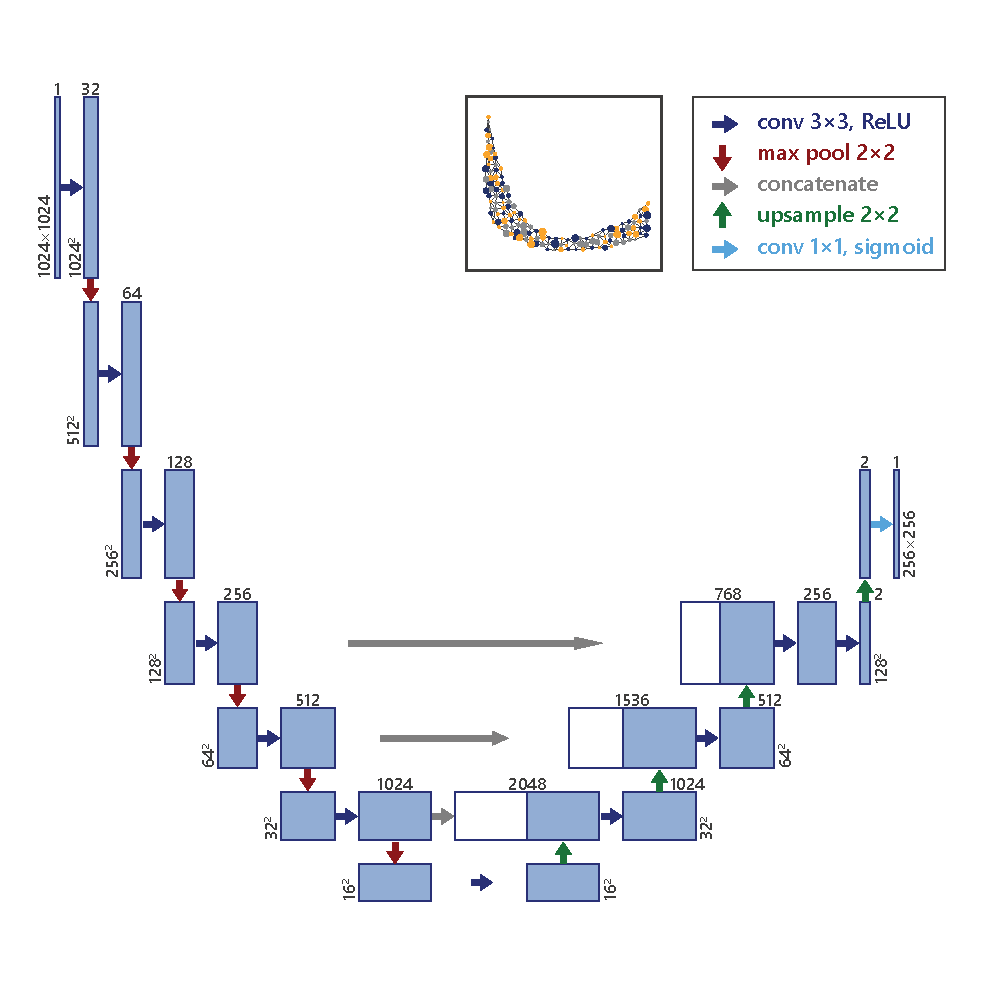
\includegraphics[width=0.95\linewidth]{chapter-4/figures_PDF/fig4-M1_architecture.pdf}
    \caption{CLEMnet architecture.
    The blue boxes correspond to multi-channel feature maps with the number of channels and image dimensions annotated above and to the side of each box, respectively. Arrows represent different possible operations as described in the legend. The asymmetric layout underlies the illustration from Figure \ref{fig:4.1_overview}B.}
    \label{fig:4M_architecture}
\end{figure}


% 4.4.3
% -----
\subsection{Data acquisition}
\label{sec:4methods_acquisition}
The integrated microscopy workflow for large-scale correlative imaging and reconstruction is described in \textcite{lane2021integrated}. Briefly, fluorescence imaging is done via the Delmic SECOM (Delmic B.V.), which has been retrofitted into the vacuum chamber of a Verios 460 SEM (Thermo Fisher Scientific) \cite{liv2013simultaneous, zonnevylle2013integration}. Correlative FM and low-magnification EM image tiles are acquired in a grid-like pattern encompassing each tissue section. The fluorescence is captured prior to EM to avoid quenching of the fluorescence. Following the acquisition of each correlative image pair, the FM tile is registered to the low-magnification EM tile by means of cathodoluminescent markers \cite{haring2017automated}. The fluorescence signal is then used to guide to regions of interest for subsequent, high-magnification EM, such as the islet of Langerhans in the case of the rat pancreas tissue. As thin sections of the mouse breast tumor cells are more or less homogeneous, acquisition areas were chosen based on minimal damage to the section. 

Each FM tile consists of a \SI{10}{\second} exposure at \SI{405}{\nano\meter} excitation for Hoechst and \SI{555}{\nano\meter} excitation for AF594. The corresponding low-magnification EM tiles are acquired at \SI{1.5}{\kilo\electronvolt} landing energy with a \SI{1}{\kilo\volt} bias potential, as described in \textcite{lane2021optimization}, with a \SI{400}{\pico\ampere} primary beam current, \SI{5}{\micro\second} dwell, and \SI{150}{\micro\meter} field width. The baseline imaging parameters for high magnification EM are the same as those for low-magnification EM with the exception of a \SI{2}{\micro\second} dwell and \SI{12}{\micro\meter} field width (${\sim}$\SI{3}{\nano\meter} pixel size). Imaging parameters for the datasets of mouse breast tumor cells acquired to assess network robustness are provided in Table \ref{tab:4M_params}. All of the image data used in this work is publicly available.\footnote{\href{https://sonic.tnw.tudelft.nl/catmaid/}{https://sonic.tnw.tudelft.nl/catmaid/}} Visualization and navigation of the large-scale datasets is made possible by CATMAID \cite{saalfeld2009catmaid}.

% --- Table 4.1 (params) ---
\begin{table}[tbh]
    \centering
    \caption{EM imaging settings used for the acquisition of resin-embedded mouse breast tumor cells. For data navigation purposes, Z index corresponds to section index within CATMAID.}
    \small
    \begin{tabular}
        {>{\raggedleft\arraybackslash}p{0.8cm} % Z
         >{\raggedleft\arraybackslash}p{2cm} % Section
         >{\raggedleft\arraybackslash}p{1cm} % LE
         >{\raggedleft\arraybackslash}p{1cm} % Dwell
         >{\raggedleft\arraybackslash}p{1cm} % PS
         >{\raggedleft\arraybackslash}p{1cm} % N
         >{\raggedleft\arraybackslash}p{1.5cm} % A
         >{\raggedleft\arraybackslash}p{1cm} % T
        }
        \toprule
        Z & Section ID & LE (eV) & Dwell (µs) & Pixelsize (nm) & N. EM images & Area\quad (µm × µm) & Time (hr) \\ 
        \midrule
        10--19 & S007A--S009C & 1500 & 2 & 3 & 484 & 234 × 234 & 4.5 \\
        0 & S002A & 1500 & 3 & 3 & 484 & 234 × 234 & 6.8 \\
        1 & S003B & 1500 & 1 & 3 & 484 & 234 × 234 & 2.3 \\
        2 & S003C & 1500 & 2 & 3 & 484 & 234 × 234 & 4.5 \\
        3 & S003D & 1500 & 2 & 4 & 289 & 241 × 241 & 2.7 \\
        4 & S004A & 1500 & 2 & 5 & 196 & 249 × 249 & 1.8 \\
        5 & S004B & 1500 & 2 & 6 & 121 & 235 × 235 & 1.1 \\
        6 & S005A & 1500 & 5 & 3 & 484 & 234 × 234 & 11.3 \\
        7 & S005B & 2000 & 2 & 3 & 484 & 234 × 234 & 4.5 \\
        8 & S006A & 1000 & 2 & 3 & 484 & 234 × 234 & 4.5 \\
        9 & S006B & 3000 & 2 & 3 & 484 & 234 × 234 & 4.5 \\
        \bottomrule
    \end{tabular}
    \label{tab:4M_params}
\end{table}


% 4.4.4
% -----
\subsection{Robustness \& validation}
\label{sec:4methods_robustness}
EM and FM image pairs are augmented during training to increase the robustness of the model. The objective is to improve the model's flexibility and to account for different types of imaging conditions rather than to extend it to different specimens. While the model may generate reasonable predictions of the fluorescence intensity on the same cell type or organelle across different specimens, it is not generalizable to tissue or cell types it has not been trained on. Several different types of data augmentation are applied to account for the variety of imaging settings the network would reasonably encounter if tested on EM data from other instruments.

% --- Affine transformation ---
\subsubsection{Affine transformation}
Affine transformations are applied to training data such that the model learns to adapt to modest changes in structural topology. By introducing minor adjustments to the rotation ($\theta$), translation ($t_x$, $t_y$), scale ($z_x$, $z_y$), and shear ($\Gamma$) of the training data, some degree of invariance to these transformations is embedded into the model \cite{simard2003best}. The applied affine transformations are randomized for each EM-FM image pair such that each image pair receives the exact same transformation (Figure \ref{fig:4M_affine}).

% --- Fig 4.M2 (affine) ---
\begin{figure}[!tbh]
    \centering
    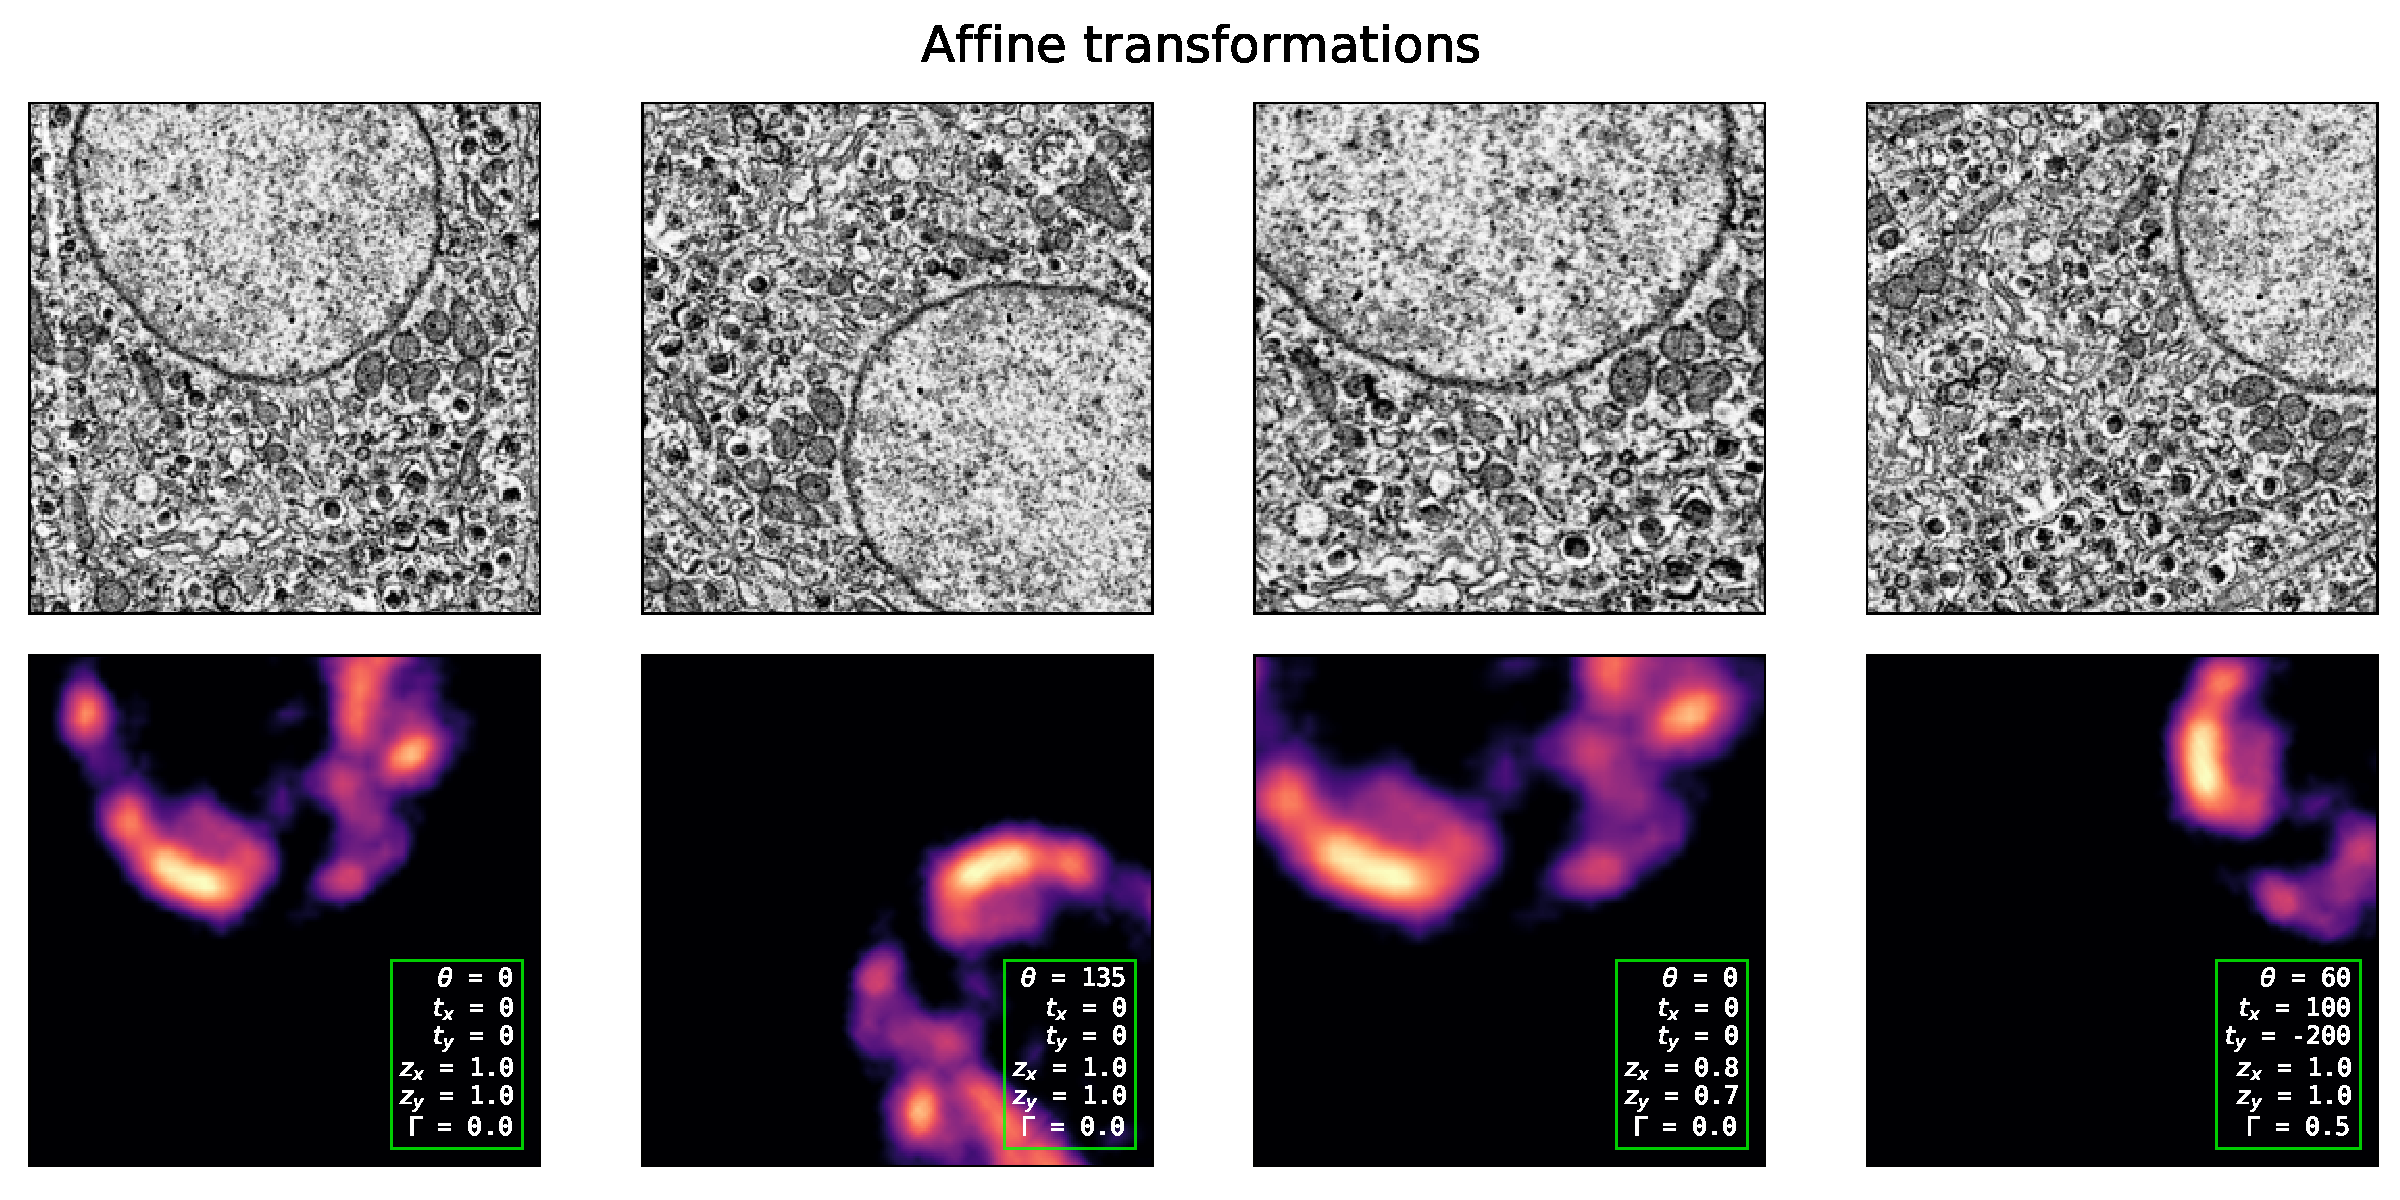
\includegraphics[width=\linewidth]{chapter-4/figures_PDF/fig4-M2_affine.pdf}
    \caption{Affine transformations are applied to the training data to render the model invariant to topological changes, resulting in greater robustness.
    The original, correlative image pair (left) may be rotated, translated, scaled, and sheared to encompass a wide variety of possible topological changes. Exact transformation parameters are provided in the text box of each transformed image pair.}
    \label{fig:4M_affine}
\end{figure}

% --- Elastic deformation ---
\subsubsection{Elastic deformation}
Elastic deformation was identified by \textcite{simard2003best} early in the development of neural networks as an effective means of augmenting training data. It was later shown by \textcite{dosovitskiy2014discriminative} and reinforced by \textcite{ronneberger2015u} as a crucial tool for enhancing CNN training, particularly in the case of limited training samples. Elastic deformations are generated by applying a non-linear warp to the image where the warp is defined by a displacement field convolved with a Gaussian kernel of standard deviation, $\sigma$, and multiplied by a scaling factor, $\alpha$ (Figure \ref{fig:4M_elastic}, top). The displacement field is initialized by a random uniform distribution where each pixel ranges from (-1, +1) with equal probability. The value for α is also randomized such that the EM images are warped with varying intensity. Distortions are more apparent along the edges of features (Figure \ref{fig:4M_elastic}, bottom).

% --- Fig 4.M3 (elastic) ---
\begin{figure}[!tb]
    \centering
    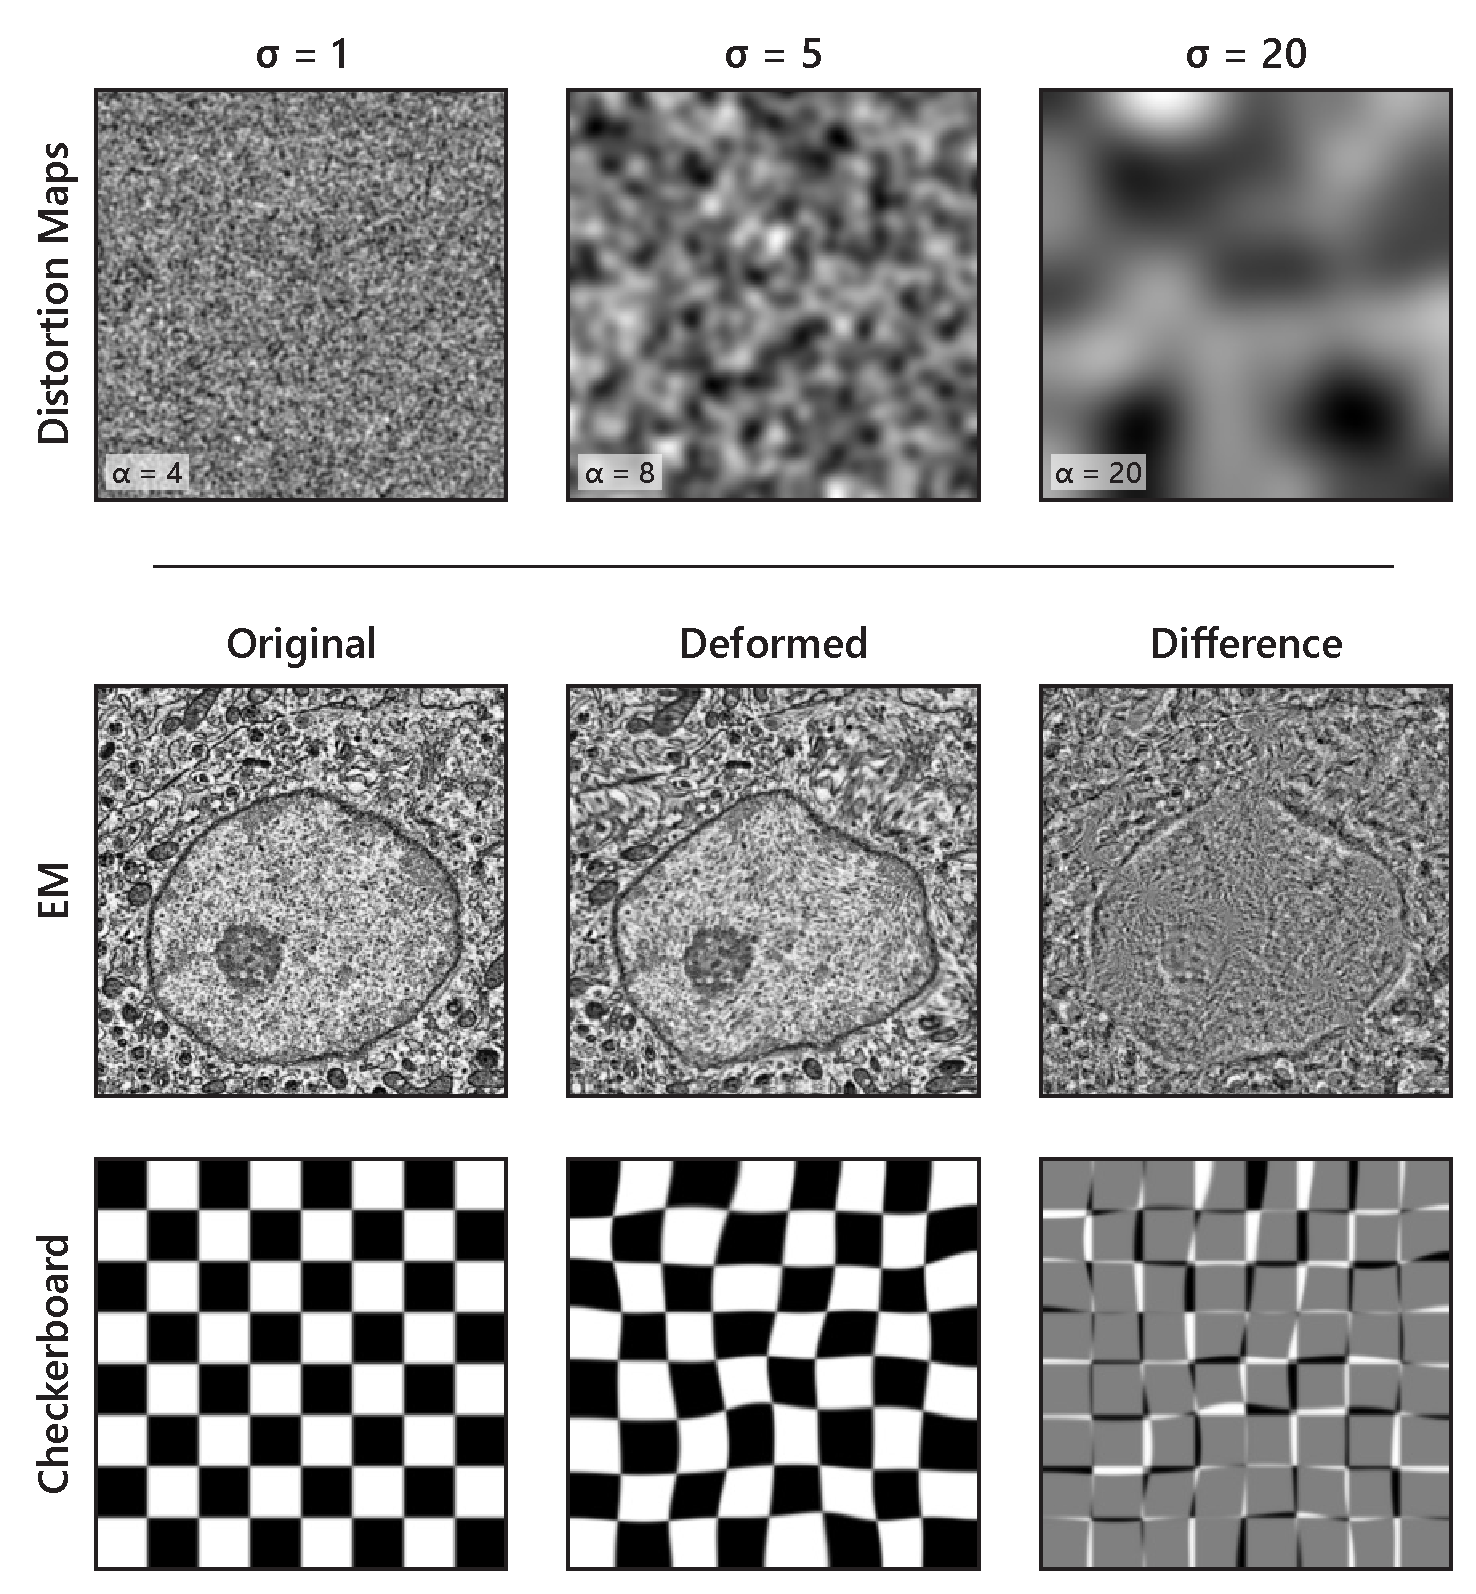
\includegraphics[width=\linewidth]{chapter-4/figures_PDF/fig4-M3_elastic.pdf}
    \caption{%
    Top: Distortion maps used for applying elastic deformations to training data. For small $\sigma$ the deformation resembles the addition of white noise, while for large $\sigma$ the deformation is more severe.
    Bottom: Elastic deformation applied to an EM training image and a checkerboard pattern.}
    \label{fig:4M_elastic}
\end{figure}

% --- Brightness / contrast ---
\subsubsection{Brightness \& contrast variation}
To account for the expected variations to brightness and contrast in EM image data acquired across different samples, microscopes, imaging settings, (day of the week), etc. the brightness and contrast levels are given a random adjustment. The brightness is varied ${\pm}$20\% by adding a gray-level bias, while the contrast is adjusted in the range $(0.75 < \delta < 1.5)$ where the value of each pixel, $x$, is scaled by
%
\begin{equation}
    (x - \bar{x})\,\delta + \bar{x}
\end{equation}
%
where $\bar{x}$ is the average intensity of the whole image.

% --- Noise augmentation ---
\subsubsection{Noise augmentation}
There are multiple sources of noise in the SEM detection chain, each with their own statistical distribution. The dominant source of noise on a properly operating SEM is, however, typically Poisson (shot noise) as additional contributions from the detector, scanning electronics, etc. tend to be much smaller than the statistical noise inherent in the signal \cite{joy2008noise}. Training images are therefore augmented with shot noise to improve the model’s robustness with respect to low SNR images (Figure \ref{fig:4M_noise}). The probability that a random variable $X$ is equal to $k$ is given by
%
\begin{equation}
    P(X=k;\lambda) = \frac{\lambda^{k} e^{-\lambda}}{k!}
\end{equation}
%
where $\lambda$ is the expectation value of $X$ as well as its variance.

% Fig 4.M4 (noise)
% ----------------
\begin{figure}[!tbh]
    \centering
    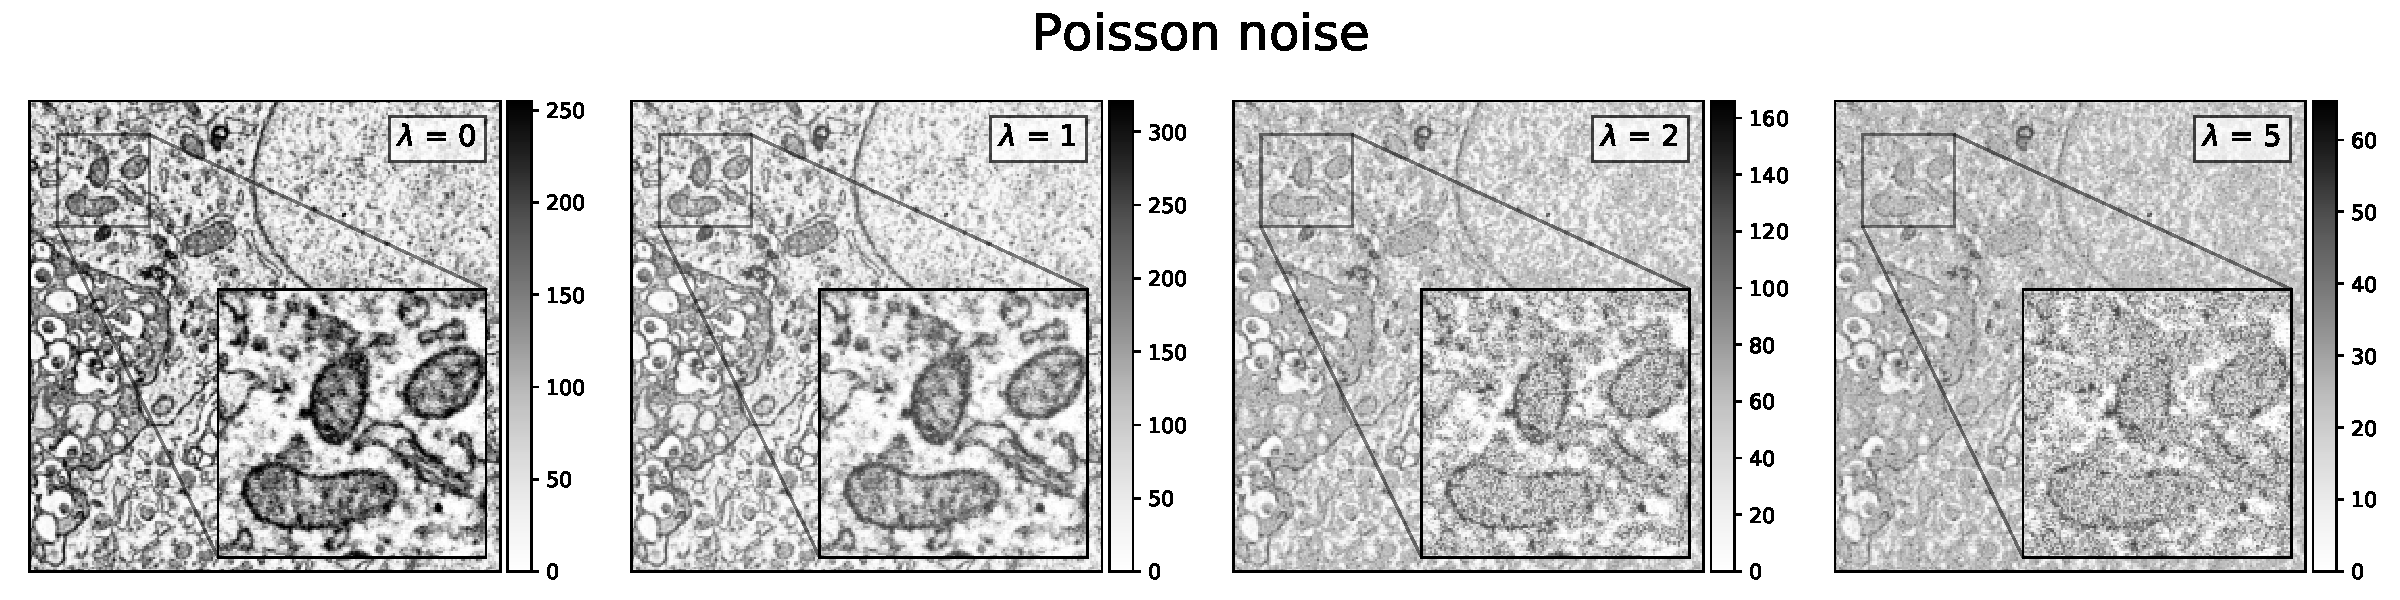
\includegraphics[width=\linewidth]{chapter-4/figures_PDF/fig4-M4_noise.pdf}
    \caption{Poisson noise added to an EM training image.
    Features become unrecognizable at high values of $\lambda$.}
    \label{fig:4M_noise}
\end{figure}


% 4.4.5
% -----
\subsection{Quantitative analysis}
\label{sec:4methods_analysis}

\subsubsection{Cell nuclei counting}
Experts and trained volunteers were asked to recognize cell nuclei in datasets comprised of fluorescence signals obtained with a microscope and generated by CLEMnet. The experts consisted of two researchers from the University Medical Center Groningen who routinely examine islets of Langerhans, while the volunteers consisted of thirteen researchers from within the TU Delft Department of Imaging Physics who were trained to recognize cell nuclei in both FM and EM image data from comparable tissue. The annotations made by the experts were weighted by a factor 3.

An unsupervised, brute-force nearest neighbors search was used to filter outlier annotations from the EM dataset. For each annotated point, the Euclidean distance to every other annotated point was calculated. If a point was found to have at least 12 neighboring points (corresponding to ${\ge}$80\% of annotators) within a radius roughly equal to the average radius of a cell nucleus, the point was kept. Points with an insufficient amount of neighboring points were discarded, resulting in clusters of point clouds corresponding to the ground truth nuclei. $k$-means clustering was then used to agglomerate point clouds from which the centroid of each cluster could be computed and added to the ground truth set.

\subsubsection{Segmentation evaluation}
Segmentation performance is evaluated by the intersection over union (IoU), a similarity coefficient used to measure the overlap of two sets $A$ and $B$.
%
\begin{equation}
    IoU(A, B) = \frac{\left|\,A \cap B\,\right|}{\left|\,A \cup B\,\right|}
\end{equation}



% 4.4.6
% -----
\subsection{Segmentation}
\label{sec:4methods_segmentation}

\subsubsection{Fully supervised segmentation}

Segmentation masks for training were generated either by manually tracing cell nuclei in EM images of rat pancreas islets (using GIMP) or by thresholding the measured fluorescence or CLEMnet prediction images. A value of 0.2 was empirically chosen to be the threshold after rescaling the intensity range from (0, 255) to (0, 1). To reduce the burden on manual tracing, a higher zoom level was chosen than for generating fluorescence predictions. 96 images from across six different sections were manually segmented. One section was set aside for testing, while the five remaining sections were divided 80\%/20\% for training and validation. Implementation of the ResNet-34 model architecture was facilitated by Segmentation Models \cite{Yakubovskiy:2019}, which provides neural network frameworks for image segmentation compatible with Keras and Tensorflow.


\subsubsection{Partial points annotation}

Labelled images are generated in a two-phase process adapted from \textcite{qu2020weakly}. In the first phase (Figure \ref{fig:5M_segmentation}A), partial points annotation is used to generate a probability map for the location of cell nuclei. Partial points annotation was performed on the same dataset as used for the fully supervised segmentation. Though all nuclei visible in the EM were annotated, only five were chosen at random for generating Gaussian masks (PP Mask). The values for the Gaussian masks are given by
%
\begin{equation}
    M_i = 
    \begin{cases}
        \text{exp}\left({-\frac{D_i^2}{2\sigma^2}}\right) & \text{if}\; D_i < r_1, \\
        0 & \text{if}\; r_1 < D_i < r_2, \\
        -1 & \text{otherwise}
    \end{cases}
\end{equation}
%
where $D_i$ is the radial distance from each pixel $i$ to the nearest partial point, $\sigma$ is the standard deviation of the Gaussian distribution over each partial point, and $r_1$ and $r_2$ are the typical nuclear radius (estimated from the validation dataset) and the outer radius of background labels, respectively. Here we have used $r_1=\text{\SI{5}{\micro\meter}}$, $r_2 = 2 r_1$, and $\sigma = r_1 / 2$. In this way each pixel is classified as either nucleus ($>\text{0}$), background (0), or remains unlabelled ($-\text{1}$).

When trained on pairs of EM images and PP masks, ResNet-34 yields probability maps of predicted nuclei locations for given input EM test images. The initial probability map, though rather crude, is used to refine the PP mask to generate a better estimate of the background. The background estimate is updated according to the conditions
%
\begin{equation}
    M^N_i = 
    \begin{cases}
        M_i & \text{if}\; D_i < r_2, \\
        0 & \text{if}\; D_i > r_2 \quad \text{and} \quad p_i < 0.1, \\
        -1 & \text{otherwise}
    \end{cases}
\end{equation}
%
where $p_i$ is the probability of that pixel belonging to the nucleus class after iteration $N$. The pipeline is designed in such a way to as to iteratively yield better and better probability maps. We find, however, that the maps tend to converge after $N=\text{2}$ for this particular dataset.

% Fig 4.M5 (segmentation)
% -----------------------
\begin{figure}[!tb]
    \centering
    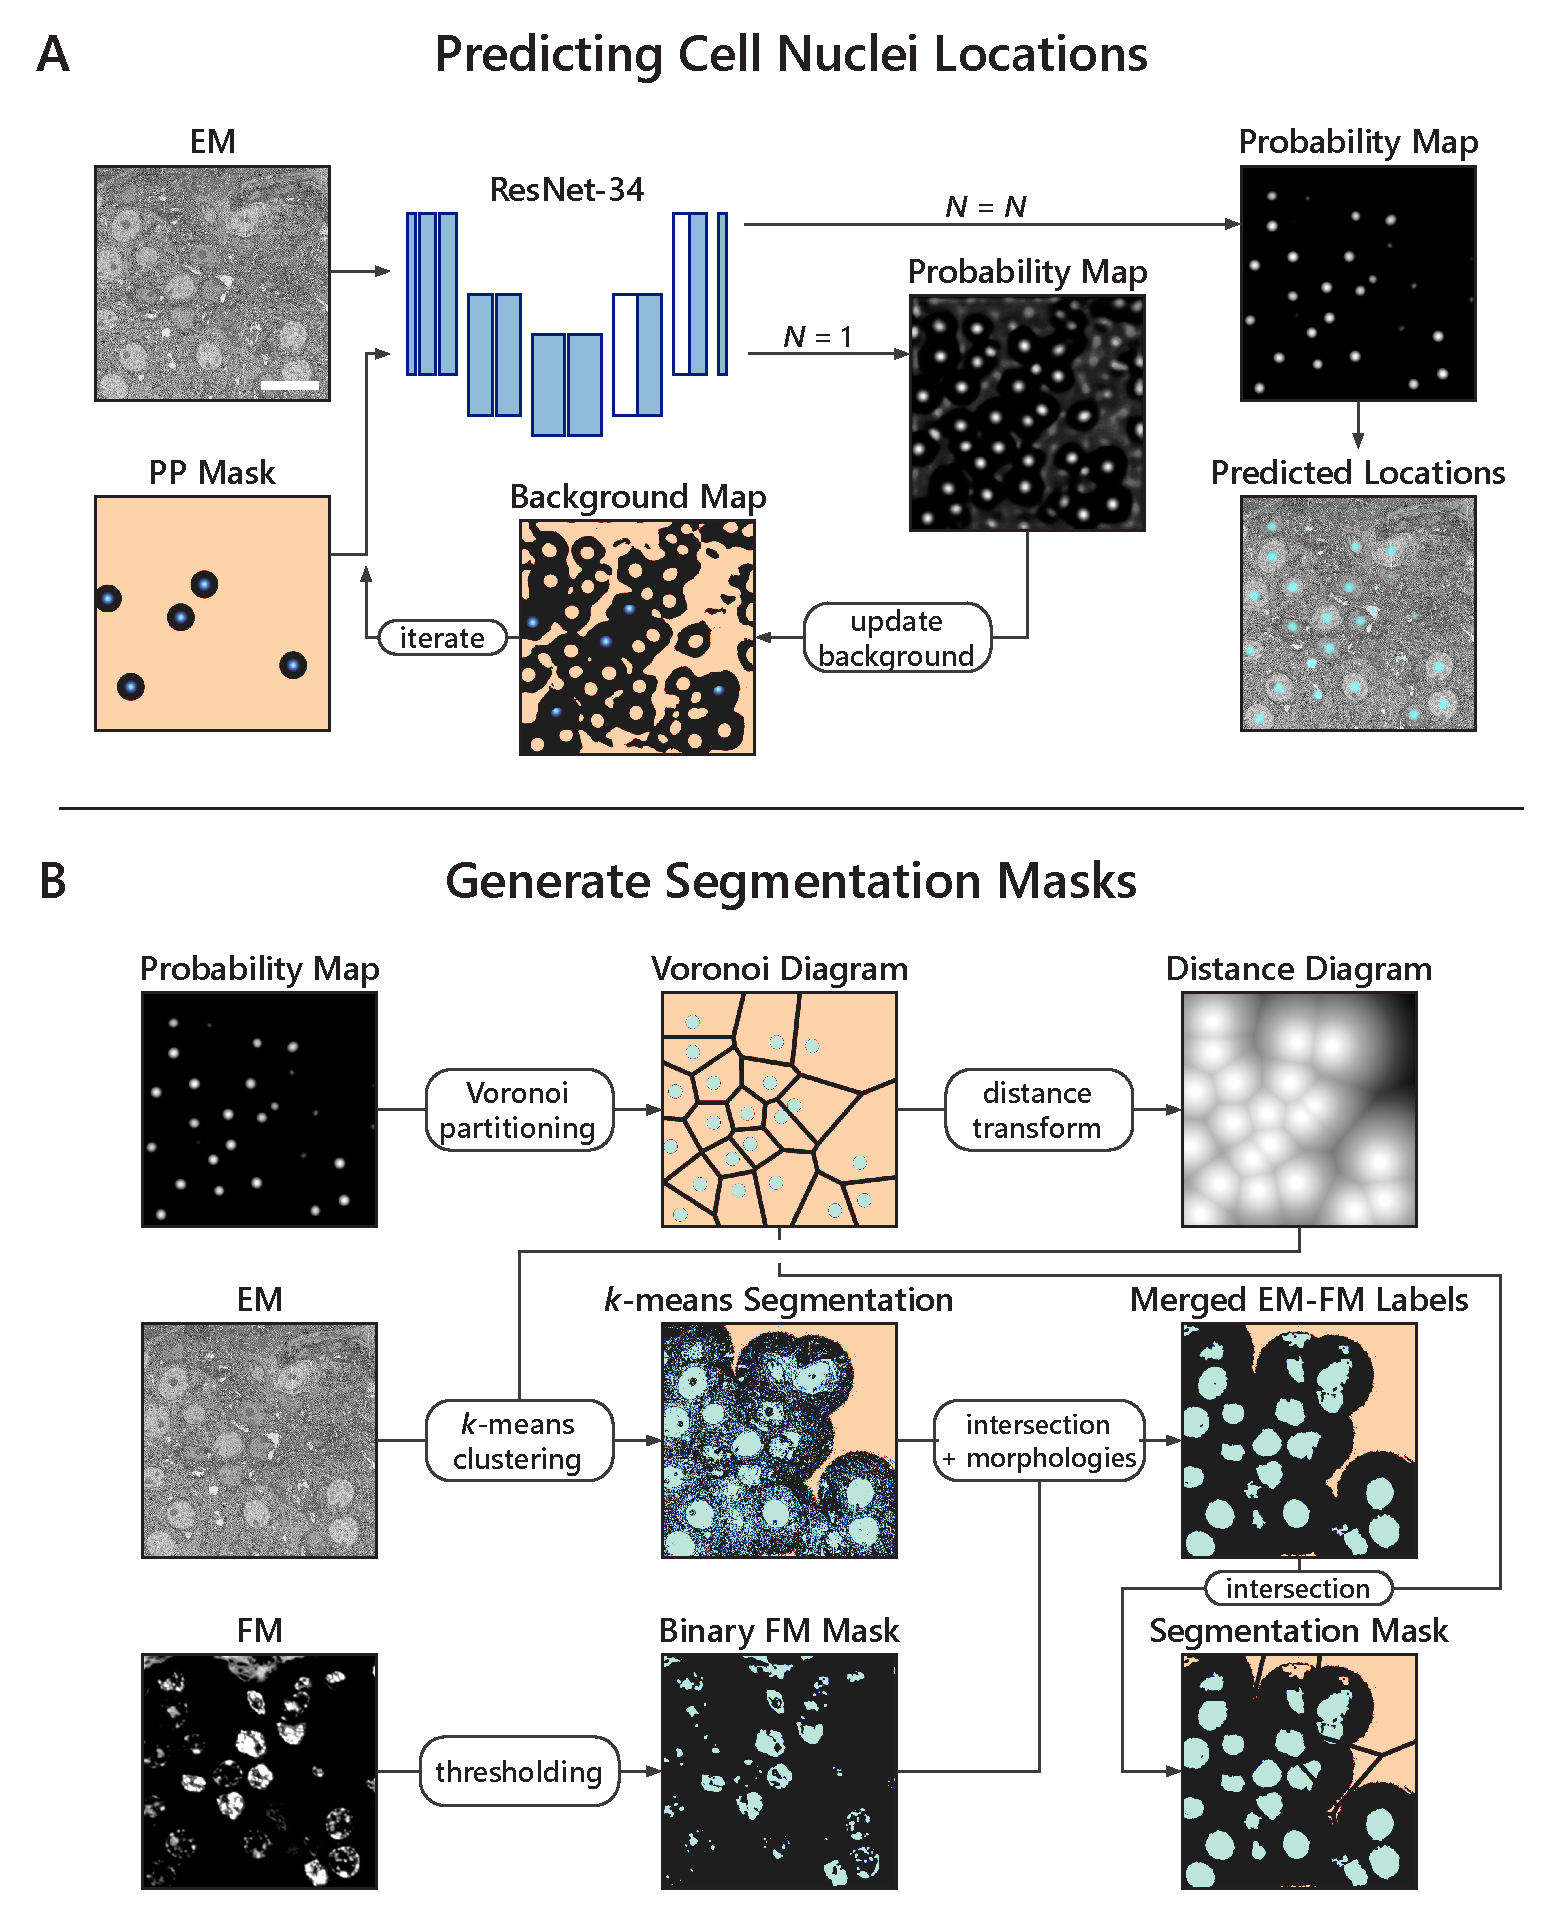
\includegraphics[width=0.90\linewidth]{chapter-4/figures_PDF/fig4-M5_segmentation.pdf}
    \caption{Semi-automated image processing pipeline for generation of segmentation masks from partial points annotation.
    (A) Partial points annotation is used to create Gaussian mask images to train an instance of ResNet-34 to predict nuclei locations. The predictions are refined through self-training to yield more accurate probability masks.
    (B) A Voronoi diagram based off of the probability map in (A) is merged with labelled images from $k$-means clustering to create segmentation masks for training a separate instance of ResNet-34 for organelle segmentation.
    Legend: white (or cyan) -- nucleus; black -- background; beige -- unlabelled.
    Scale bar: \SI{10}{\micro\meter}.}
    \label{fig:5M_segmentation}
\end{figure}

In phase two (Figure \ref{fig:5M_segmentation}B), segmentation masks are generated by a combination of $k$-means clustering and a Voronoi partitioning of the nuclei detected in phase one. These two labelling schemes are complementary to one another. $k$-means clustering preserves the spatial information in the EM image, providing the contour of the nuclei at the expense of having greater uncertainty, while the Voronoi partition provides accurate nuclei localization at the expense of underestimating the background label. The EM image is multiplied by the distance transform of the Voronoi diagram prior to $k$-means clustering to amplify nuclei. Clustering is then done with $k=\text{3}$. We choose to subtract a value of 1 from the resulting image such that the background goes to $-\text{1}$ (unlabelled). In this way the model does not train on regions of the image where a label cannot easily be inferred from either the $k$-means clustering or Voronoi partitioning. These regions are typically in the void between adjacent nuclei where it can be disadvantageous to make an assumption on whether a pixel belongs to the nucleus or background class, as it is possible that a nucleus was missed in phase one.

The fluorescence image is independently thresholded and intersected with the $k$-means clustered image. Small segments are removed via morphological opening, closing, and erosion operations. Larger segments are filtered by convexity, measured as the ratio of the area of each segment relative to the area of its convex hull. Segments with convexity less than 0.85 become unlabelled. Lastly, the merged labels from $k$-means clustering of the EM and thresholding of the FM are intersected with the Voronoi diagram to result in a final segmentation mask. Pairs of segmentation masks and EM images are then used to train an instance of ResNet-34 for organelle segmentation in the same manner as was described for fully supervised segmentation. Note that the fluorescence image was originally included as a separate channel during $k$-means clustering, but the results from doing so were marginally worse: final IoU score of 67\% vs 72\%.

\clearpage
\section{Supplementary material}
\label{sec:4_supplement}
\renewcommand{\thefigure}{S\arabic{figure}}
\setcounter{figure}{0}    

% Figure 4.S1 (ROIS)
% ------------------
\begin{figure}[!tbh]
    \centering
    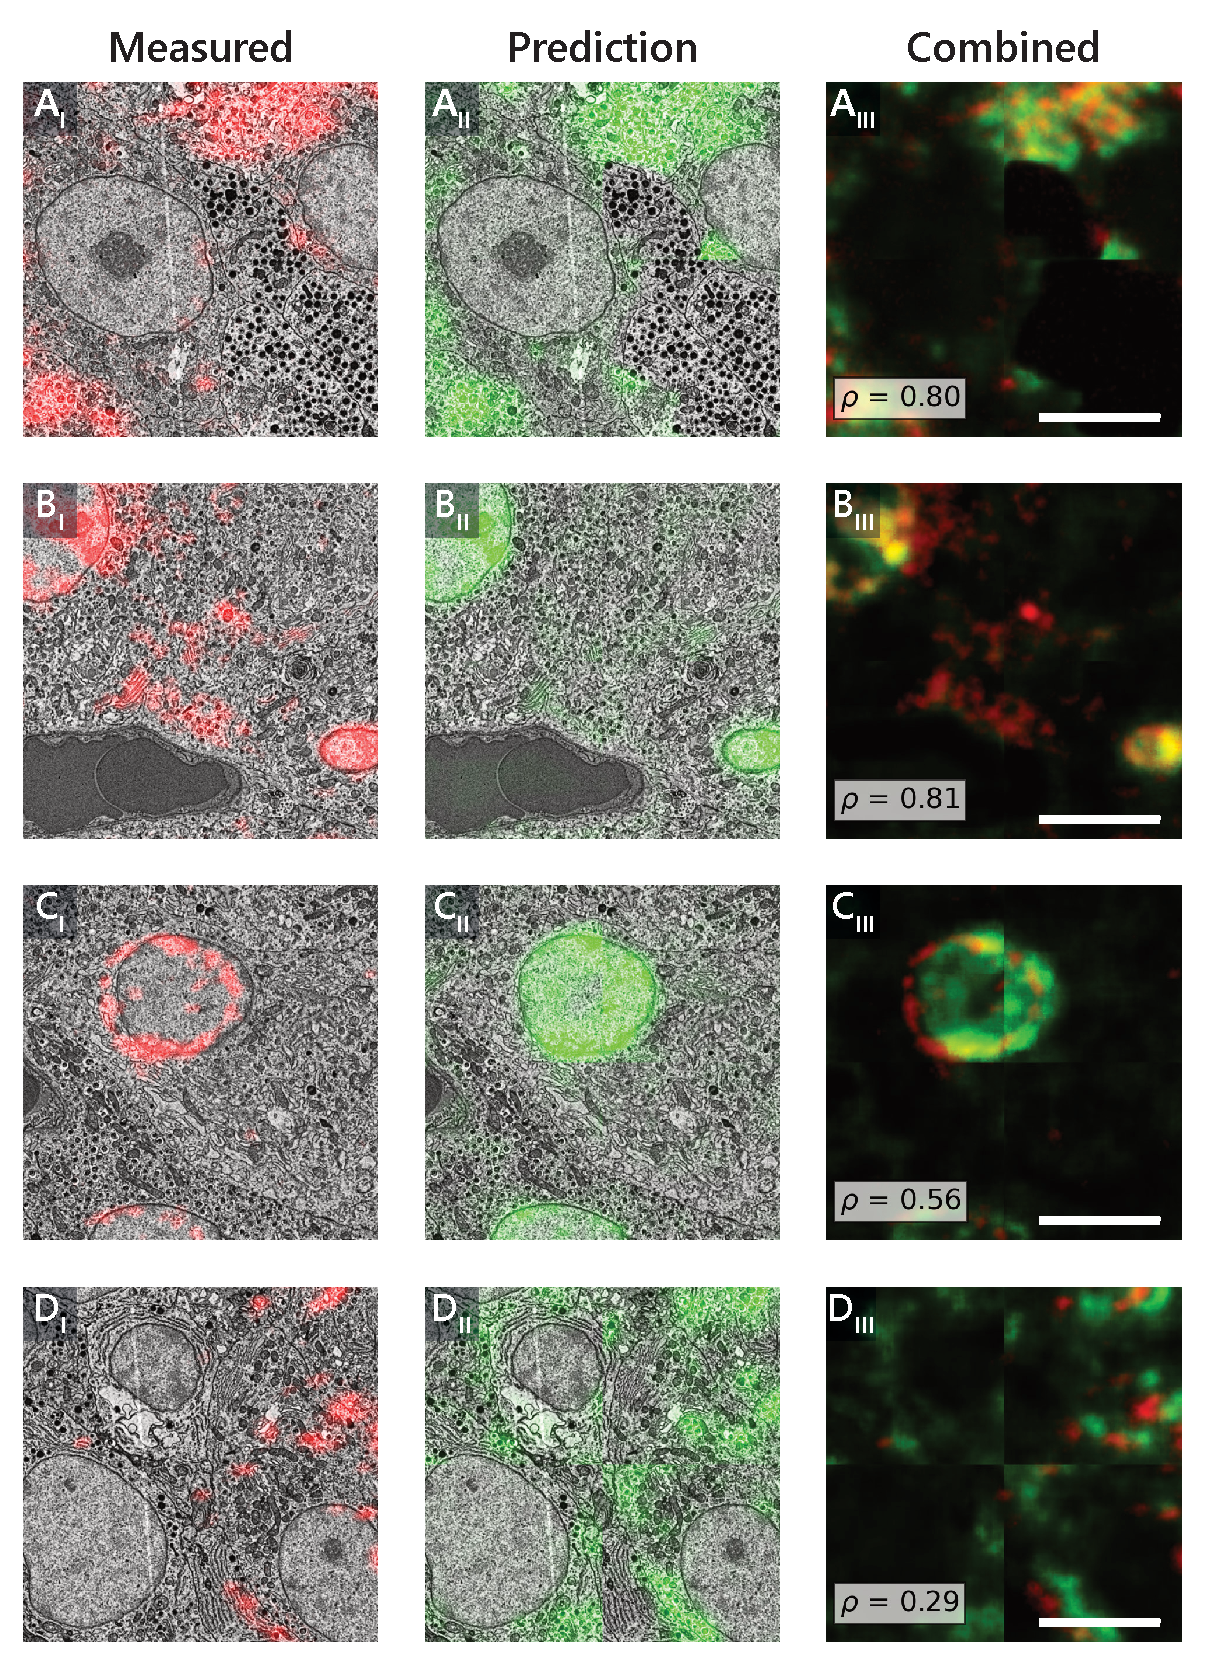
\includegraphics[width=0.95\linewidth]{chapter-4/figures_PDF/fig4-S1_rois.pdf}
    \caption{CLEMnet is able to perform nontrivial structural recognition tasks as well as mitigate issues inherent to fluorescence imaging. (Continued on next page\ldots)}
    \label{fig:4.S1_rois}
\end{figure}
\addtocounter{figure}{-1}
\begin{figure}
    \caption{For each selected ROI (A-D), the measured fluorescence (left, red) and prediction (center, green) are overlaid onto the EM, and combined to show overlap and differences in signal intensity (right).
    (A) The network is able to distinguish between insulin and similar-looking glucagon granules, a difficult task for non-experts.
    (B) An instance of AF594 emission from \SI{405}{\nano\meter} Hoechst excitation demonstrates that the network prediction is less susceptible to bleedthrough. 
    (C) As the network generates predictions directly on structures within the EM, it is able to compensate for errors in the EM-FM registration near the edges of the field of view where the registration may be extrapolated.
    (D) The network is for the same reason also less susceptible to off-axis aberrations such as vignetting, which results in diminished signal at the corners of the fluorescence field of view.
    Note that several predictions are stitched together to compose the predicted image shown, at times giving rise to edge artefacts.
    Scale bars: (A--D) \SI{5}{\micro\meter}.}
\end{figure}

\quad


% TODO:
%   Captions for supplemental figs
%   Decide whether to include SNR validation/notebooks
%   Reverse x-axis in Figure S1
%   Bigger font in Figure S2
%   Make final pdfs for figures
%   Final readthrough


% References
\printbibliography[title={References}]
\end{refsection}
  % stage bias
% Reset section and figure counters
\renewcommand\thesection{\arabic{chapter}.\arabic{section}}
\renewcommand{\thefigure}{3.\arabic{figure}}
\setcounter{figure}{0}


\chapter[Integrated array tomography]{Integrated array tomography for 3D correlative light and electron microscopy}
\label{chap:3}

% Abstract
\begin{abstract}
    Volume electron microscopy (EM) of biological systems has grown exponentially in recent years due to innovative large-scale imaging approaches. As a standalone imaging method, however, large-scale EM typically has two major limitations: slow rates of acquisition and the difficulty to provide targeted biological information. We developed a 3D image acquisition and reconstruction pipeline that overcomes both of these limitations by using a widefield fluorescence microscope integrated inside of a scanning electron microscope. The workflow consists of acquiring large field of view fluorescence microscopy (FM) images, which guide to regions of interest for successive EM (integrated correlative light and electron microscopy). High precision EM-FM overlay is achieved using cathodoluminescent markers. We conduct a proof-of-concept of our integrated workflow on immunolabelled serial sections of tissues. Acquisitions are limited to regions containing biological targets, expediting total acquisition times and reducing the burden of excess data by tens or hundreds of GBs.
\end{abstract}

% Published as footnote
\blfootnote{This chapter has been published as: \fullcite{lane2021integrated}.}
\clearpage


% Sections
\section{Introduction}
\label{sec:4.1_intro}


% Motivate from EM perspective
% bio-insight from EM is hard
% CLEM has been developed to assist

Electron microscopy (EM) has transformed the way in which biologists understand intra- and inter-cellular systems. Due to the lack of inherent biological specificity, however, interpretation of EM datasets typically requires tedious expert analysis and annotation. For this reason, fluorescence microscopy (FM) is often used in conjunction with EM, complementing structural data with targeted biological labels. Fluorescent labelling, however, comes with several drawbacks. Sample preparation protocols are often laborious, time-consuming, and potentially damaging to the sample. Protocols must also be adapted to limit concentrations of heavy metal staining if intermediate processing of the sample is to be avoided \cite{kuipers2015scanning,lane2021optimization}. Fluorescent labelling is also susceptible to bleedthrough when multiple fluorophores are expressed in a single sample as well as varying specificity---Hoechst dyes, for instance, bind to both DNA and RNA. Furthermore, registering the separate imaging modalities across large spatial extents remains a technically challenging and primarily manual task \cite{russell20173d} [other references]. Correlative fluorescence and electron microscopy experiments are therefore typically limited in scope to the micron or tens of microns scale, and thus so are the regions for which biological labels can be provided \cite{russell20173d} [other references].

As recognition of organelles and other subcellular structures remains a pivotal obstacle in biological EM, we questioned whether large-scale EM datasets could be supplemented with biological labels through alternate means. To address this question, we sought to leverage recent advances in deep learning. Deep convolutional neural networks (CNN) in particular have been shown to be capable of inferring complex, non-linear relationships from image data \cite{he2016deep,januszewski2018high}. Prior work involving deep CNNs in the context of electron microscopy data has primarily been limited to applications in segmentation, denoising, and compressed sensing \cite{ede2021deep}. Semantic segmentation, the classification of pixels into discrete categories, does ultimately serve the purpose of adding biological labels to EM data. However, modern deep learning approaches require hours of tedious expert segmentation \cite{huang2014identifying,heinrich2018synaptic,liu2020automatic,spiers2021deep}. In order for \textcite{heinrich2020automatic} to amass sufficient training data for organelle segmentation, it required one person two weeks of manual segmentation per \SI{1}{\micro\meter^3} volume of image data; 28 blocks of this size were manually annotated in total to enable whole cell organelle segmentation.

Although relatively little attention has been paid to alternative applications in deep learning for EM data, recent work has focused on generating biological labels from other imaging modalities. \textcite{christiansen2018silico} designed a deep neural network to predict fluorescence labels from transmitted light images. \textcite{ounkomol2018label} extended the technique to generate 3D fluorescence from stacks of transmitted light microscopy data and further demonstrated the possibility of predicting immunofluorescence from EM images in order to facilitate automatic registration of fluorescence data with EM. To address the challenge of adding biological specificity to large-scale EM datasets, we thus explored the potential for a CNN to make label-free fluorescence predictions from electron microscopy image data.

In this work we present a deep CNN developed for generating fluorescence predictions on large-scale EM data of tissue and cellular samples. We demonstrate the performance of our model on thin sections of rat pancreas tissue, which have been immunolabelled with Alexa Fluor 594 and given a Hoechst counterstain, as well as Hoechst-stained sections of resin-embedded HeLa cells. Network predictions are quantitatively evaluated against corresponding true fluorescence images based on the Pearson correlation coefficient (PCC, or $\rho$) as well as by assessing human recognition of fluorescence predictions on cell nuclei. We additionally assess the network's robustness by measuring its predictive power on EM datasets acquired with varying imaging parameters. Finally, we explore the potential of correlative and predicted fluorescence signals for use as labels in segmentation experiments.






% \subsection{Things we will show}
% \begin{itemize}[noitemsep]
%     \item Can train a CNN to predict fluorescence based on registered CLEM images as training data
%     \begin{itemize}
%         \item Demonstrate on rat pancreas tissue: cell nuclei and insulin granules (micron scale and sub-diffraction limit)
%         \item Demonstrate on zebrafish: cell nuclei
%         \item Demonstrate on mouse heart tissue: phospholamban labelled with TRITC
%         \item Validate with PCC etc.\ and manual counting (for rat pancreas cell nuclei only)
%     \end{itemize}

%     \item CLEMnet is robust
%     \begin{itemize}
%         \item Predictions can be made on different rats
%         \item Predictions can be made on lower signal images (lower dwell) when trained with noise augmentation
%     \end{itemize}

%     \item CLEMnet predictions can be used for (semi/fully)-automated segmentation
%     \begin{itemize}
%         \item CLEMnet data slightly outperforms CLEM data for segmenting cell nuclei
%         \item Caveat that segmentation falls short of manual segmentation
%     \end{itemize}
% \end{itemize}




% Deep convolutional neural networks (CNN) are capable of inferring complex, non-linear relationships between images. Prior work applying deep learning strategies to EM data has often revolved around segmentation tasks. Competitions such as the IEEE International Symposium on Biomedical Imaging (ISBI) challenge for segmentation of neuronal structures in electron microscopic stacks \cite{arganda2015crowdsourcing} have inspired generations of neural network architecture development such as the U-net \cite{ronneberger2015u} and its 3D counterpart \cite{cciccek20163d}. More recently, a CNN has been employed for for whole cell organelle segmentation in a micron-sized volumetric EM dataset \cite{heinrich2020automatic}. Relatively little attention has been paid to alternative applications of deep learning algorithms for volumetric EM data. \textcite{ounkomol2018label} trained a model to facilitate automatic registration of multichannel fluorescence data to EM array tomography data. % Limited to myelin. [More examples].




% As recognition of organelles and other subcellular structures remains a pivotal obstacle in biological EM, [lots and lots of work] has centered around segmentation and classification of these structures. More recently, these efforts have focused on employing deep learning strategies to infer [descriptive adjective] patterns from EM image data rich in structural information \cite{heinrich2020automatic} [25 references therein]. [only expert-level people would otherwise be capable of discerning].
% %
% Competitions such as the IEEE International Symposium on Biomedical Imaging (ISBI) challenge for segmentation of neuronal structures in electron microscopic stacks \cite{arganda2015crowdsourcing} have inspired generations of neural network architecture development such as the U-net \cite{ronneberger2015u} and its 3D counterpart \cite{cciccek20163d}. More recently, a CNN has been employed for whole cell organelle segmentation in a micron-sized volumetric EM dataset \cite{heinrich2020automatic}.


% %
% [No one(?) is making use of multimodal datasets to assist in recognition and segmentation of EM datasets]. 



\section{Material \& methods}
\label{sec:3.2_methods}


% 3.2.1
% -----
\subsection{Tissue and sample preparation}
\label{sec:3M_prep}
Rat pancreas was prepared as follows: fresh pancreas was cut from an \SI{83}{day} old rat into small pieces and fixed in 4\% paraformaldehyde (PFA; Merck) + 0.1\% glutaraldehyde (GA; Polysciences) as described in \textcite{ravelli2013destruction}. A complete zebrafish larva (\SI{120}{hpf}) was fixed in 2\% PFA + 2\% GA. Both samples were post-fixed in 1\% osmium tetroxide and 1.5\% potassium ferricyanide in \SI{0.1}{M} cacodylate buffer, dehydrated through ethanol and embedded in EPON (Serva). \SI{100}{\nano\meter} serial sections were cut and placed onto formvar-covered ITO-coated glass coverslips (Optics Balzers). Immunolabeling was performed as described previously \cite{kuipers2015scanning}. Samples were etched with 1\% periodic acid for \SI{10}{\minute}, followed by a \SI{30}{\minute} blocking step: 1\% bovine serum albumin (BSA; Sanquin, Netherlands) in tris-buffered saline (TBS), pH 7.4. Next, anti-insulin was incubated for \SI{2}{\hour} (guinea pig; 1:50, Invitrogen, PA1-26938, RRID: AB\_794668, for rat pancreas and anti-insulin; 1:100, Abcam, ab210560, for zebrafish pancreas), followed by washing and subsequent incubation for \SI{1}{\hour} with biotinylated secondary antibody (donkey-anti-guinea pig; 1:400, Jackson Immunoresearch, for rat pancreas and goat-anti-rabbit; 1:400, Dako, for zebrafish pancreas) followed by washing steps. Finally, streptavidin conjugated AF594 (1:100, Jackson Immunoresearch, for rat pancreas) and streptavidin conjugated TRITC (1:100, Jackson Immunoresearch, for zebrafish pancreas) were added for \SI{1}{\hour} followed by washing.


% 3.2.2
% -----
\subsection{Digital light microscopy}
\label{sec:3M_keyence}
The sections, after being placed on the ITO-coated glass slide, are imaged at \SI{30}{X} magnification (${\sim}$\SI{7}{\micro\meter\per\pixel}) using a VHX-6000 digital light microscope (Keyence) operating in reflection mode. To capture every section on the \SI{22}{\milli\meter} $\times$ \SI{22}{\milli\meter} ITO-coated glass slide, a 3 $\times$ 3 grid of RGB images is acquired and automatically stitched together.


% 3.2.3
% -----
\subsection{Integrated microscopy}
\label{sec:3M_integrated}
The integrated microscope is a widefield SECOM fluorescence microscope (Delmic B.V.) retrofitted into the vacuum chamber of a Verios 460 SEM (Thermo Fisher Scientific) \cite{liv2013simultaneous, zonnevylle2013integration}. The microscopes share a common optical axis, translation stage, and control software. FM images are obtained with \SI{10}{\second} exposures, recorded by a Zyla 4.2 sCMOS camera (Andor - Oxford Instruments). Excitation wavelengths of \SI{405}{\nano\meter} and \SI{555}{\nano\meter} are used to excite Hoechst and AF594. The SECOM is equipped with a CFI S Plan Fluor ELWD 60XC (\SI{0.70}{NA}) objective (Nikon), which allows for long working distance imaging (\SIrange{1.8}{2.6}{\milli\meter}), to prevent electrical breakdown in vacuum, which must be accounted for due to the presence of high electric fields induced by the stage bias \cite{vos2021retarding}.

SEM imaging is conducted in two rounds: (1) low-magnification (\SI{38}{\nano\meter\per\pixel}) scans accompanying each fluorescent acquisition; (2) high-magnification (\SI{5}{\nano\meter\per\pixel}) acquisitions on ROI identified by fluorescence expression. Both low and high magnification imaging are performed at \SI{2.5}{\kilo\electronvolt} primary beam energy with a \SI{-1}{\kilo\volt} bias potential applied to the sample stage such that the landing energy is \SI{1.5}{\kilo\electronvolt}, which proved optimal for ${\sim}$\SI{100}{\nano\meter} sections. The negative potential bias enhances the backscattered electron (BSE) signal, which is collected by the insertable concentric backscattered detector (Thermo Fisher Scientific) \cite{lane2021optimization}.


% 3.2.4
% -----
\subsection{Alignment and reconstruction software}
Image data from the integrated microscope is uploaded to a local storage server running an instance of render-ws,\footnote{\href{https://github.com/saalfeldlab/render}{https://github.com/saalfeldlab/render}} a collection of open-source web services for rendering transformed image tiles. The tiles and their respective metadata are organized into stacks, configured as MongoDB databases. The alignment routines are arranged in a series of Jupyter notebooks,\footnote{\href{https://github.com/hoogenboom-group/iCAT-workflow}{https://github.com/hoogenboom-group/iCAT-workflow}} which parse the image metadata for the EM-FM overlay as well as make calls to render-ws via a python wrapper (render-python\footnote{\href{https://github.com/AllenInstitute/render-python}{https://github.com/AllenInstitute/render-python}}). EM image stitching and volume alignment are based on the scale-invariant feature transform (SIFT)---an algorithm designed to detect and match local features in corresponding images \cite{lowe1999object}. SIFT features are stored in render-ws databases where they can be processed by BigFeta,\footnote{\href{https://github.com/AllenInstitute/BigFeta}{https://github.com/AllenInstitute/BigFeta}} a linear least squares solver for scalable 2D and 3D image alignment based on point correspondences. CLEM datasets are ultimately exported to CATMAID \cite{saalfeld2009catmaid} for google-maps-like visualization. 3D visualizations are done in Fiji \cite{schindelin2012fiji} using the Volume Viewer plugin.\footnote{\href{https://imagej.net/plugins/volume-viewer}{https://imagej.net/plugins/volume-viewer}}

\section{Results}
\label{sec:3.3_results}


\section{Discussion}
\label{sec:3.4_discussion}

A new workflow for integrated array tomography for the semi-automated acquisition and reconstruction of volume CLEM data is presented. High-resolution EM is limited to select ROI by targeting areas based on fluorescence expression. This not only expedites acquisition time, but eases the burden on data management requirements. Interpretation of EM data is in turn facilitated by the addition of fluorescent labels. The workflow demonstrated here extends the work of \textcite{liv2013simultaneous}, which introduced the integrated microscope, and \textcite{haring2017automated}, which presented the fiducial-free CL registration procedure, to targeted correlative imaging of serial sections. \textcite{gabarre2021workflow} presented an alternative method for integrated array tomography in which light microscopy and EM are combined to localize structures through a series of feedback loops. Our approach differs in several ways. First, fluorescence imaging is done \textit{in-vacuo} as opposed to transmitted light microscopy done at ambient pressure. This allows for more automated EM-FM (or EM-LM) overlay, as the CL registration procedure can only be done in high vacuum \cite{haring2017automated}. Additionally, the multi-modal alignment methodology conceived here offers a more scalable solution for generating volumetric CLEM data. Integrated array tomography was inspired in part by the multi-scale approach of \textcite{hildebrand2017whole}, in which full brain EM imaging of a larval zebrafish was conducted by selecting ROI for subsequent acquisition based on inspection between imaging rounds. In this work, conversely, ROI are identified by \textit{in-situ} fluorescence, bypassing the need for post-processing and alignment between magnification scales.

On-section immunofluorescence and fluorescent staining constitute viable options for FM imaging of resin-embedded sections in high vacuum. Pancreas tissue in particular is well-suited for immunofluorescence due to the prevalence of insulin epitopes. While in both nature and technique development, immunolabeling approaches are always dependent on the capacity for antibodies and epitopes to interact, this is typically inefficient for most antibodies, and particularly so for EPON-embedded sections. We find that approximately 1 in 10 antibodies tested in our lab are applicable for EPON labeling. While acrylic resins (e.g. Lowicryl, LR White) have been shown to be more compatible with immunolabeling, a trade-off must be made between the strength of the fluorescence signal and the quality of the ultrastructure \cite{watanabe2011protein, paez2015fixation}. Complications with serial sectioning and ultrastructure preservation (beyond that shown in the zebrafish pancreas) arose when experimenting with Lowicryl; hence EPON was selected as the embedding medium for this study.

Probes typically used for live FM, such as fluorescent proteins, are likewise incompatible with conventional EM sample preparation techniques \cite{de2015correlated}. Although protocols have been developed for retaining fluorescence post-embedding \cite{kukulski2011correlated, watanabe2011protein, peddie2014correlative, fu2020meosem}, the same compromises exist between fluorescence retention and ultrastructure preservation. Fluorescent proteins have the additional limitation that the specimen must be genetically modified, rendering them unsuitable for use in native animals and humans. In-resin fluorescence preservation thus remains a challenge—only made more difficult by imposing high vacuum conditions, which may lower fluorescence intensities for biological probes typically optimized for use in aqueous environments \cite{peddie2014correlative}. We are nevertheless confident that future developments in fluorescent proteins and embedding media will present compelling opportunities to apply integrated array tomography to a variety of biological questions.

We foresee that the multimodal datasets obtained using this method will be instrumental in forthcoming machine learning applications \cite{eckstein2020microtubule, liu2020automatic, heinrich2021whole}. Thus far, applications of registered EM-FM datasets appear to be limited to facilitating registration of sequential CLEM data using artificial predictions for the fluorescence signal \cite{ounkomol2018label, seifert2020deepclem}. Volume EM datasets, particularly in connectomics, are now routinely segmented via deep convolutional neural networks \cite{buhmann2021automatic, heinrich2021whole}. Acquisition rates and manual annotation of datasets, however, both serve as bottlenecks for reconstructing dense networks of cells and organelles \cite{kornfeld2018progress}. Given its ability to provide labeled biological information as well as reduce imaging volumes to select regions, integrated array tomography is poised to deliver significant gains in this arena.

Future work will be directed towards further refinement and automation. The CL registration procedure could be made more robust by illuminating the sample with a greater number of CL spots or by increasing the camera integration time. Updates to the alignment software could furthermore allow for the distortion field correction used in \textcite{haring2017automated} to achieve sub-\SI{5}{\nano\meter} overlay precision. Cutting sections manually remains a significant bottleneck for throughput, as it is prone to error and requires expert training \cite{wanner2015challenges}. We expanded from a single section to nine, to 63, and have now placed more than 100 serial sections onto ITO-coated coverslips. Increasing beyond ${\sim}$\SI{10}{\micro\meter} of biological material, however, is cumbersome without more sophisticated sectioning techniques such as automated tape-collecting ultramicrotome (ATUM) \cite{hayworth2014imaging} or magnetic collection \cite{templier2019magc}. These may introduce their respective complications; ATUM, for example, is designed to collect sections on (opaque) Kapton tape. More extensive automation strategies can alternatively be applied to the correlative imaging pipeline. \textcite{delpiano2018automated} devised a way to automatically detect fluorescent cells using an integrated light and electron microscope. We envision a workflow for fully automated integrated array tomography in which fluorescent ROIs are automatically recognized, navigated to, and acquired, rendering three-dimensional CLEM datasets tailored to answer the specific biological research question.

\clearpage
\section{Supplementary material}
\label{sec:4_supplement}
\renewcommand{\thefigure}{S\arabic{figure}}
\setcounter{figure}{0}    

% Figure 4.S1 (ROIS)
% ------------------
\begin{figure}[!tbh]
    \centering
    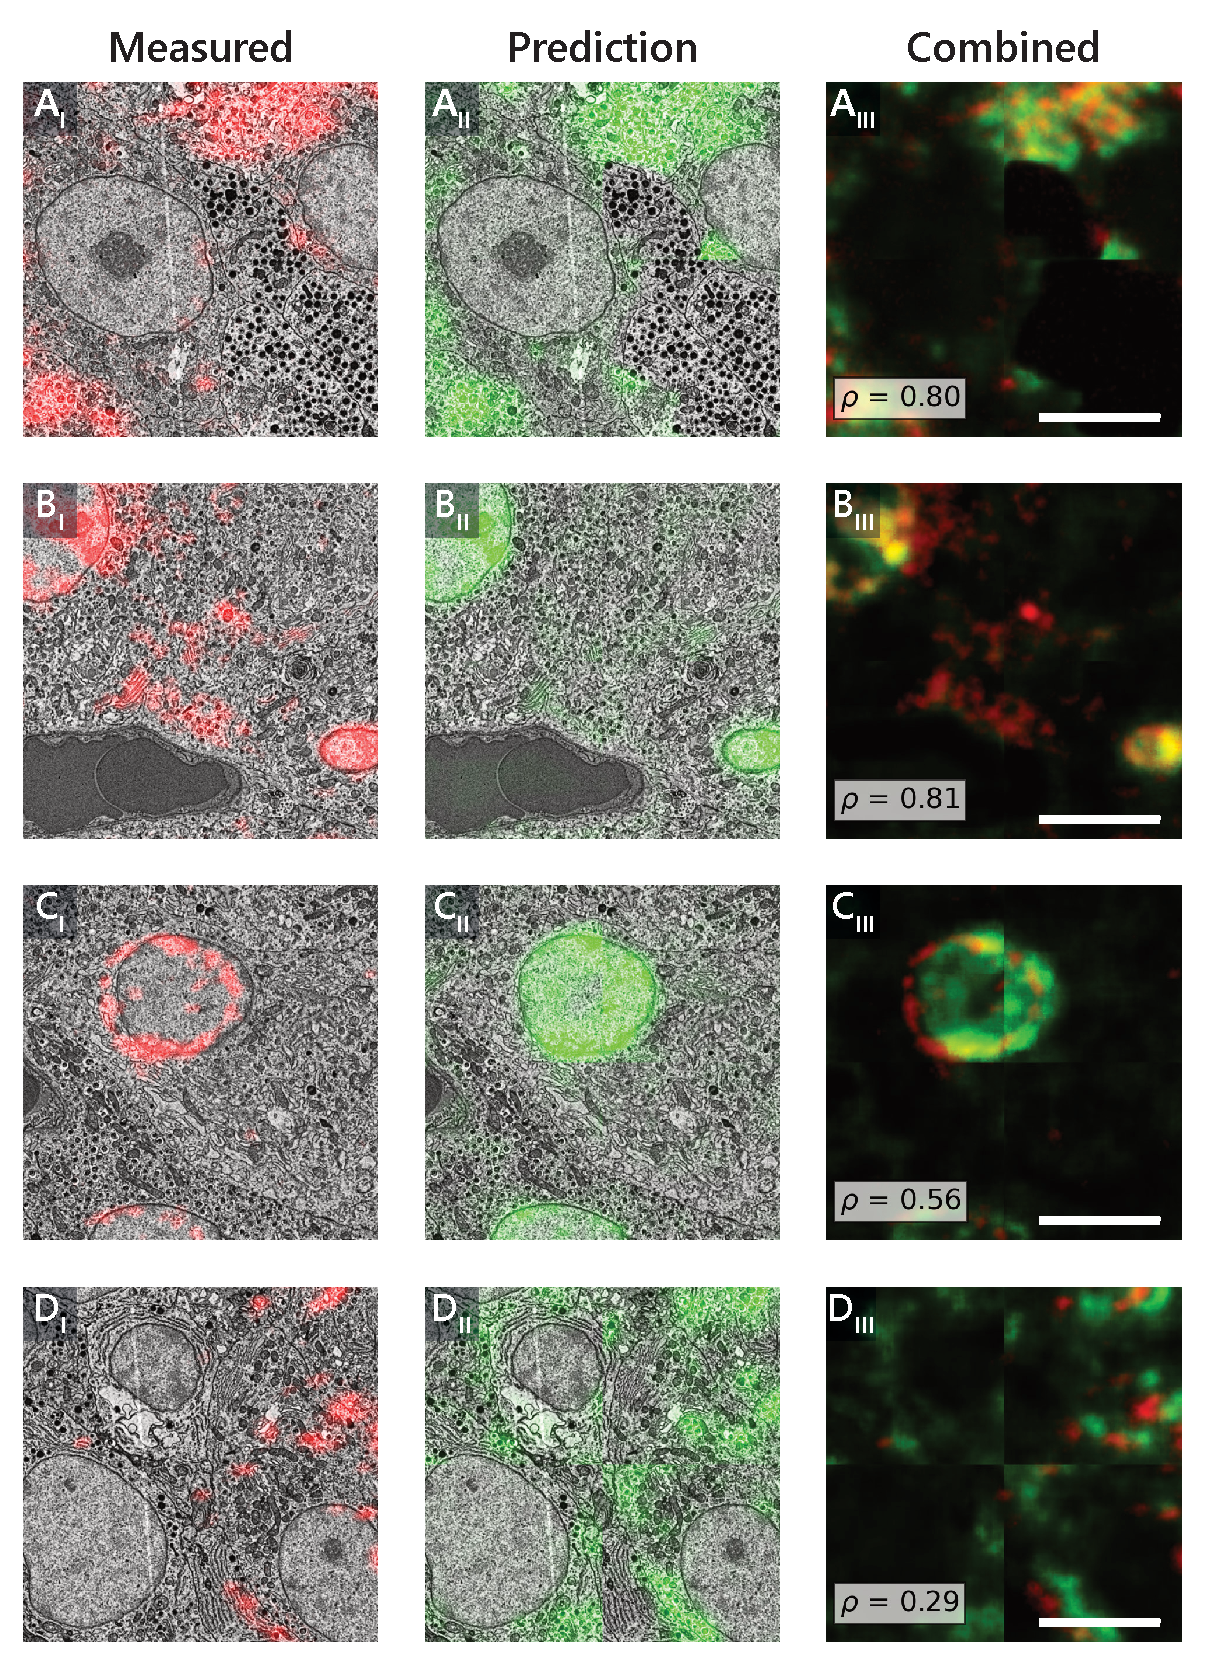
\includegraphics[width=0.95\linewidth]{chapter-4/figures_PDF/fig4-S1_rois.pdf}
    \caption{CLEMnet is able to perform nontrivial structural recognition tasks as well as mitigate issues inherent to fluorescence imaging. (Continued on next page\ldots)}
    \label{fig:4.S1_rois}
\end{figure}
\addtocounter{figure}{-1}
\begin{figure}
    \caption{For each selected ROI (A-D), the measured fluorescence (left, red) and prediction (center, green) are overlaid onto the EM, and combined to show overlap and differences in signal intensity (right).
    (A) The network is able to distinguish between insulin and similar-looking glucagon granules, a difficult task for non-experts.
    (B) An instance of AF594 emission from \SI{405}{\nano\meter} Hoechst excitation demonstrates that the network prediction is less susceptible to bleedthrough. 
    (C) As the network generates predictions directly on structures within the EM, it is able to compensate for errors in the EM-FM registration near the edges of the field of view where the registration may be extrapolated.
    (D) The network is for the same reason also less susceptible to off-axis aberrations such as vignetting, which results in diminished signal at the corners of the fluorescence field of view.
    Note that several predictions are stitched together to compose the predicted image shown, at times giving rise to edge artefacts.
    Scale bars: (A--D) \SI{5}{\micro\meter}.}
\end{figure}

\quad


% References
\printbibliography[title={References}]
  % iCAT
% \chapter[Label-free fluorescence predictions]{Label-free fluorescence predictions from large-scale correlative light and electron microscopy data}
\label{chap:4}

% Abstract
\begin{abstract}
    Electron microscopy (EM) provides high-resolution images of (sub-)cellular ultrastructure. Identifying particular organelles or proteins of interest from EM images alone, however, is often a challenge.
    Deep learning-based approaches have rapidly been adopted within biological EM to perform structural recognition tasks, such as organelle segmentation, due to their strength in pattern inference and analyzing visual imagery.
    Such approaches require large training datasets, typically at the expense of hundreds of hours of human annotation.
    As an alternative means of providing biological labels to EM datasets, we developed CLEMnet, a deep convolutional neural network that has been trained on large-scale ({$\sim$}\SI{16}{GB}) correlative light and electron microscopy (CLEM) data. 
    % These datasets have been compiled via integrated array tomography such that manual annotation and segmentation has been removed from the workflow.
    CLEMnet predictions generated on EM images unseen by the network are highly correlated with the measured fluorescence signal.
    We additionally assess the feasibility of the correlative fluorescence data and network-generated predictions as training masks for organelle segmentation.
\end{abstract}

\blfootnote{This chapter is in preparation for a manuscript to be submitted for publication: \fullcite{lane2022label}.}
\clearpage

% Sections
\section{Introduction}
\label{sec:4.1_intro}


% Motivate from EM perspective
% bio-insight from EM is hard
% CLEM has been developed to assist

Electron microscopy (EM) has transformed the way in which biologists understand intra- and inter-cellular systems. Due to the lack of inherent biological specificity, however, interpretation of EM datasets typically requires tedious expert analysis and annotation. For this reason, fluorescence microscopy (FM) is often used in conjunction with EM, complementing structural data with targeted biological labels. Fluorescent labelling, however, comes with several drawbacks. Sample preparation protocols are often laborious, time-consuming, and potentially damaging to the sample. Protocols must also be adapted to limit concentrations of heavy metal staining if intermediate processing of the sample is to be avoided \cite{kuipers2015scanning,lane2021optimization}. Fluorescent labelling is also susceptible to bleedthrough when multiple fluorophores are expressed in a single sample as well as varying specificity---Hoechst dyes, for instance, bind to both DNA and RNA. Furthermore, registering the separate imaging modalities across large spatial extents remains a technically challenging and primarily manual task \cite{russell20173d} [other references]. Correlative fluorescence and electron microscopy experiments are therefore typically limited in scope to the micron or tens of microns scale, and thus so are the regions for which biological labels can be provided \cite{russell20173d} [other references].

As recognition of organelles and other subcellular structures remains a pivotal obstacle in biological EM, we questioned whether large-scale EM datasets could be supplemented with biological labels through alternate means. To address this question, we sought to leverage recent advances in deep learning. Deep convolutional neural networks (CNN) in particular have been shown to be capable of inferring complex, non-linear relationships from image data \cite{he2016deep,januszewski2018high}. Prior work involving deep CNNs in the context of electron microscopy data has primarily been limited to applications in segmentation, denoising, and compressed sensing \cite{ede2021deep}. Semantic segmentation, the classification of pixels into discrete categories, does ultimately serve the purpose of adding biological labels to EM data. However, modern deep learning approaches require hours of tedious expert segmentation \cite{huang2014identifying,heinrich2018synaptic,liu2020automatic,spiers2021deep}. In order for \textcite{heinrich2020automatic} to amass sufficient training data for organelle segmentation, it required one person two weeks of manual segmentation per \SI{1}{\micro\meter^3} volume of image data; 28 blocks of this size were manually annotated in total to enable whole cell organelle segmentation.

Although relatively little attention has been paid to alternative applications in deep learning for EM data, recent work has focused on generating biological labels from other imaging modalities. \textcite{christiansen2018silico} designed a deep neural network to predict fluorescence labels from transmitted light images. \textcite{ounkomol2018label} extended the technique to generate 3D fluorescence from stacks of transmitted light microscopy data and further demonstrated the possibility of predicting immunofluorescence from EM images in order to facilitate automatic registration of fluorescence data with EM. To address the challenge of adding biological specificity to large-scale EM datasets, we thus explored the potential for a CNN to make label-free fluorescence predictions from electron microscopy image data.

In this work we present a deep CNN developed for generating fluorescence predictions on large-scale EM data of tissue and cellular samples. We demonstrate the performance of our model on thin sections of rat pancreas tissue, which have been immunolabelled with Alexa Fluor 594 and given a Hoechst counterstain, as well as Hoechst-stained sections of resin-embedded HeLa cells. Network predictions are quantitatively evaluated against corresponding true fluorescence images based on the Pearson correlation coefficient (PCC, or $\rho$) as well as by assessing human recognition of fluorescence predictions on cell nuclei. We additionally assess the network's robustness by measuring its predictive power on EM datasets acquired with varying imaging parameters. Finally, we explore the potential of correlative and predicted fluorescence signals for use as labels in segmentation experiments.






% \subsection{Things we will show}
% \begin{itemize}[noitemsep]
%     \item Can train a CNN to predict fluorescence based on registered CLEM images as training data
%     \begin{itemize}
%         \item Demonstrate on rat pancreas tissue: cell nuclei and insulin granules (micron scale and sub-diffraction limit)
%         \item Demonstrate on zebrafish: cell nuclei
%         \item Demonstrate on mouse heart tissue: phospholamban labelled with TRITC
%         \item Validate with PCC etc.\ and manual counting (for rat pancreas cell nuclei only)
%     \end{itemize}

%     \item CLEMnet is robust
%     \begin{itemize}
%         \item Predictions can be made on different rats
%         \item Predictions can be made on lower signal images (lower dwell) when trained with noise augmentation
%     \end{itemize}

%     \item CLEMnet predictions can be used for (semi/fully)-automated segmentation
%     \begin{itemize}
%         \item CLEMnet data slightly outperforms CLEM data for segmenting cell nuclei
%         \item Caveat that segmentation falls short of manual segmentation
%     \end{itemize}
% \end{itemize}




% Deep convolutional neural networks (CNN) are capable of inferring complex, non-linear relationships between images. Prior work applying deep learning strategies to EM data has often revolved around segmentation tasks. Competitions such as the IEEE International Symposium on Biomedical Imaging (ISBI) challenge for segmentation of neuronal structures in electron microscopic stacks \cite{arganda2015crowdsourcing} have inspired generations of neural network architecture development such as the U-net \cite{ronneberger2015u} and its 3D counterpart \cite{cciccek20163d}. More recently, a CNN has been employed for for whole cell organelle segmentation in a micron-sized volumetric EM dataset \cite{heinrich2020automatic}. Relatively little attention has been paid to alternative applications of deep learning algorithms for volumetric EM data. \textcite{ounkomol2018label} trained a model to facilitate automatic registration of multichannel fluorescence data to EM array tomography data. % Limited to myelin. [More examples].




% As recognition of organelles and other subcellular structures remains a pivotal obstacle in biological EM, [lots and lots of work] has centered around segmentation and classification of these structures. More recently, these efforts have focused on employing deep learning strategies to infer [descriptive adjective] patterns from EM image data rich in structural information \cite{heinrich2020automatic} [25 references therein]. [only expert-level people would otherwise be capable of discerning].
% %
% Competitions such as the IEEE International Symposium on Biomedical Imaging (ISBI) challenge for segmentation of neuronal structures in electron microscopic stacks \cite{arganda2015crowdsourcing} have inspired generations of neural network architecture development such as the U-net \cite{ronneberger2015u} and its 3D counterpart \cite{cciccek20163d}. More recently, a CNN has been employed for whole cell organelle segmentation in a micron-sized volumetric EM dataset \cite{heinrich2020automatic}.


% %
% [No one(?) is making use of multimodal datasets to assist in recognition and segmentation of EM datasets]. 



\section{Results}
\label{sec:2.2_results}

% 2.2.1
% -----
\subsection{Negative bias potential enhances signal in routine EM samples}

We first illustrate how the use of a potential bias can improve signal collection in a typical SEM experiment. A potential bias of \SI{-1}{\kilo\volt} is applied to the stage of an SEM with an integrated fluorescence microscope (Figure \ref{fig:2.1_setup}A \& B). The bias is applied via an external power supply connected to a custom stage plate such that the sample is electrically isolated from the rest of the fluorescence microscope and electrical components of the stage \cite{vos2021retarding}. By generating an electric field between the sample and the BSE detector, the bias potential accelerates signal electrons inwards away from their otherwise linear trajectories. Because of their lower energy, secondary electrons (<\,\SI{50}{\electronvolt}) are redirected inside the inner annulus of the BSE detector, while higher energy backscattered electrons (>\,\SI{50}{\electronvolt}) are redirected over a wider area depending on their initial emission angle and energy.

Pancreas tissue was prepared for integrated fluorescence-electron microscopy as described in Section \ref{sec:2.4.2_sampleprep}. No post-staining was applied resulting in lower contrast relative to other EM sample preparation protocols \cite{kuipers2015scanning}. EM images of EPON-embedded, \SI{80}{\nano\meter} tissue were acquired in immersion mode with and without a \SI{-1}{\kilo\volt} bias potential (Figure \ref{fig:2.1_setup}A \& B). When subject to a bias potential, EM images demonstrate noticeably higher contrast and less noise (Figure \ref{fig:2.1_setup}C \& G). The primary beam energy was increased by \SI{1}{\kilo\volt} such that the landing energy was held constant at \SI{1.5}{\kilo\electronvolt} in accordance with the section thickness. Data acquired with increased primary energy but without the use of stage bias (Figure \ref{fig:2.1_setup}D) reveals that the increase in apparent signal does not arrive solely from an increased primary energy. Moreover, the importance of maintaining a sufficiently low landing energy becomes clear by the visible artefacts from the ITO-coated glass substrate that appear with higher energies. The \SI{0.4}{\nano\ampere} beam current and \SI{5}{\micro\second\per\pixel} dwell time are held constant in each acquisition. The gain of the BSE detector had to be decreased while applying the negative bias to prevent the detector from saturating.

% Figure 2.1 (setup)
% -----------------
\begin{figure}[!tb]
    \centering
    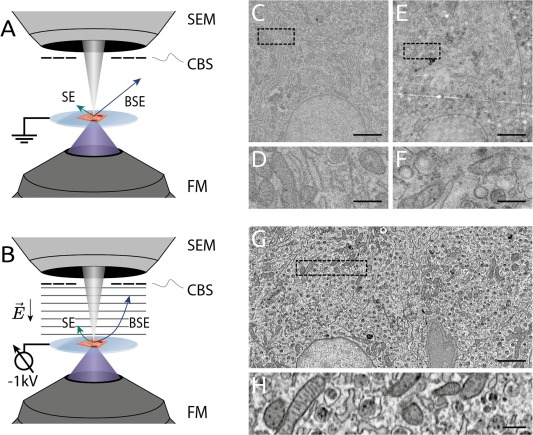
\includegraphics[width=\linewidth]{chapter-2/figures_JPEG_LQ/fig2-1_setup.jpg}
    \caption{Negative bias potential significantly enhances EM contrast in tissue. Schematic of integrated microscope without (A) and with (B) an applied stage bias. Electric field induced by the bias potential accelerates electrons emitted from the sample to the CBS detector. EM images of rat pancreas tissue without (C -- F) and with (G \& inset H) the use of stage bias. Biased images (G \& inset H) were acquired at \SI{2.5}{\kilo\electronvolt} primary energy with a \SI{-1}{\kilo\volt} bias potential---hence, a \SI{1.5}{\kilo\electronvolt} landing energy. For the sake of comparison, unbiased images (C \& inset D) were acquired with the same landing energy, while unbiased images (E \& inset F) were acquired with the same primary energy. The per-pixel dwell is held constant across all images at \SI{5}{\micro\second}. Vast improvement in EM signal and contrast can be seen by comparing insets (D \& F) with (H). Scale bars: \SI{2}{\micro\meter} (C, E, \& G); \SI{0.5}{\micro\meter} (D, F, \& H). Raw data at full resolution is available at \href{www.nanotomy.org}{Nanotomy}.}
    \label{fig:2.1_setup}
\end{figure}


% 2.2.2
% -----
\subsection{Simulating signal electron trajectories with and without negative potential bias}

% Figure 2.2 (simulations)
% ------------------------
\begin{figure}[!tb]
    \centering
    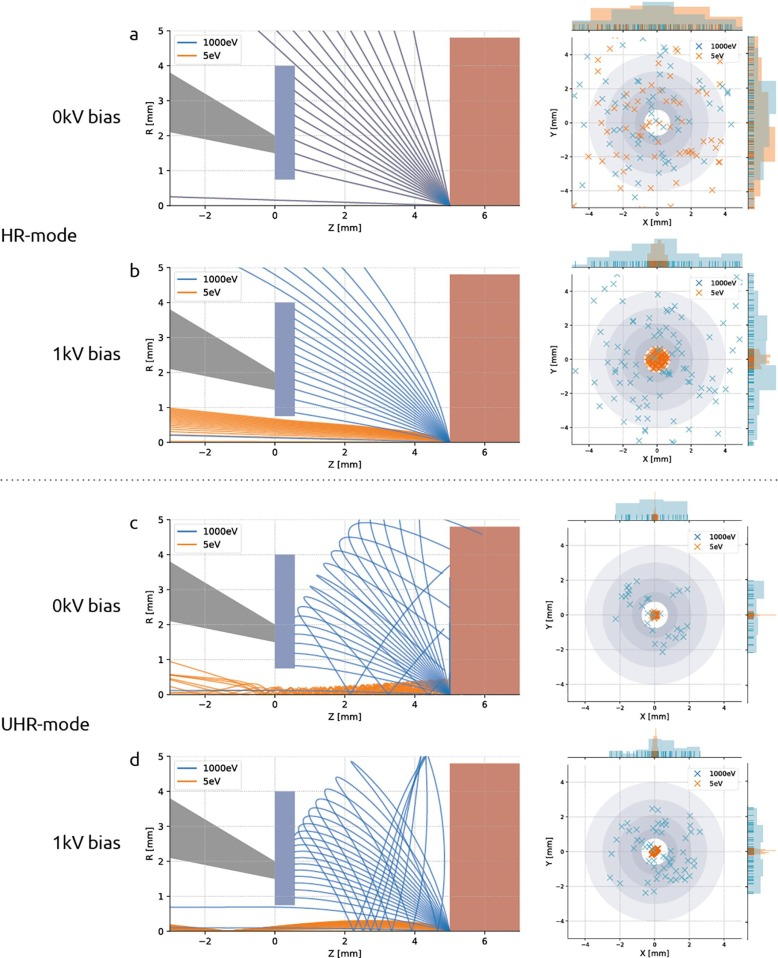
\includegraphics[width=0.85\linewidth]{chapter-2/figures_JPEG_LQ/fig2-2_simulations.jpg}
    \caption{Signal electron trajectories demonstrate the efficacy of stage bias in redirecting BSEs to the detector while simultaneously filtering out secondary electrons. Trajectory plots for SE and BSE bundles launched from the sample plane (left) and scatter plots (right) show the spatial distribution of signal electrons at the detector plane. In HR-mode, SEs and BSEs travel in overlapping, linear paths without the presence of an electric field (A), but BSEs get accelerated towards the detector when a negative bias potential is introduced (B). Signal electrons take on spiral trajectories in the presence of an immersion magnetic field (C), but are again steered to the detector when an electric field is added (D). In each set of simulations, BSEs (blue) and SEs (orange) are launched from the sample plane at $z =$ \SI{5}{\milli\meter}. Trajectory plots show geometry of the pole piece (grey), CBS detector (blue), and stage plate (red). Scatter plots show $x, y$ coordinates of signal electrons at the detector plane ($z =$ \SI{5}{\milli\meter}). Spatial distributions of signal electrons are plotted on the margins of the scatter plots.}
    \label{fig:2.2_simulations}
\end{figure}

Electron trajectories were simulated to better ascertain how a negative bias potential may give rise to better signal detection. Secondary electron and backscattered electron (BSE) trajectories were simulated for a variety of EM imaging conditions (Figure \ref{fig:2.2_simulations}). A model of the optical layout within the integrated microscope was developed in Electron Optical Design (EOD) \cite{lencova2008new} incorporating the geometry of the Verios 460 SEM objective lens and concentric backscatter (CBS) detector. The negative potential bias is factored into the model by implementing the sample plane as an additional lens element, which can then be biased to an arbitrary voltage. To mirror the \SI{5}{\milli\meter} working distance of our microscope, the end of the pole piece (grey element in Figure \ref{fig:2.2_simulations}) and start of the sample plane (red) are situated at $z=$ \SI{0}{\milli\meter} and $z=$ \SI{5}{\milli\meter} respectively. The roughly \SI{0.5}{\milli\meter} thick CBS detector (blue) is then located immediately below the pole piece.

Simulations were done for both non-immersion (high resolution or HR) and immersion (ultra-high resolution or UHR) SEM operation modes. For the case of non-immersion mode (Figure \ref{fig:2.2_simulations}A \& B), the magnetic focusing field is contained within the objective lens and therefore does not play a role in the signal electron trajectories. In these instances, the trajectories of the SEs and BSEs are dictated entirely by their initial velocity and the electric field due to the bias potential. In UHR-mode (Figure \ref{fig:2.2_simulations}C \& D), however, the sample is immersed in a strong magnetic field that both focuses the primary beam and---together with the electric field---alters the paths taken by the signal electrons. For this reason, the magnetic field strength is calculated by the field strength required to focus a parallel beam propagating in the $+z$ direction at the sample plane.

For each scenario shown, a bundle of secondary ($E_0 =$ \SI{5}{\electronvolt}) and backscattered electrons ($E_0 =$ \SI{1}{\kilo\electronvolt}) is emitted from the origin at $z =$ \SI{5}{\milli\meter}. The angular distribution is given by Lambert's cosine distribution \cite{reimer1998emission}. A screen is placed at the detector plane to record the radial position of the signal electrons, from which the scatter plots are generated (Figure \ref{fig:2.2_simulations}). The grey rings of varying diameter represent the individual segments of the CBS detector. For the case of non-immersion mode and no potential bias (Figure \ref{fig:2.2_simulations}A), the region between the detector and sample planes is field-free and the signal electrons travel freely in straight paths coinciding with one another. Only when a bias potential is added (Figure \ref{fig:2.2_simulations}B) do the higher energy BSEs diverge from the secondaries, which, due to their low initial energy, are accelerated inside the BSE detector before they are able to spread out radially. The trajectories change when under the influence of a magnetic immersion field (Figure \ref{fig:2.2_simulations}C) in which case the Lorentz force causes the signal electrons to spiral about the optical axis \cite{mullerova2009collection}. The low energy SEs remain tightly coiled as they propagate up through the BSE detector while the higher energy BSEs stretch out over greater radial distances. Whether the BSEs collide into the detector depends largely on the emission angle. The addition of a \SI{1}{\kilo\volt} bias potential (Figure \ref{fig:2.2_simulations}D) enables BSEs with a wider distribution of emission angles to reach the detector, resulting in the collection of more signal. These results suggest no secondary electron is ever registered as a count by the BSE detector---either because it is accelerated inside the detector or (in the field-free case) because it is of too little energy to generate an electron-hole pair \cite{vsakic2011boron}.

The collection efficiency of BSEs increases monotonically with increasing negative bias potential for both imaging modes (Figure \ref{fig:2.S1_percentages}). These results agree with what is suggested by the trajectory plots of Figure \ref{fig:2.2_simulations}---that the electric field generated by the stage bias tapers the radial spread of the BSEs leading to a greater percentage of BSEs collected. Note that the percentage of BSEs detected is greater for HR-mode across the range of bias potentials simulated. It therefore seems advantageous to prefer non-immersion mode, however, greater collection efficiency is only one factor to consider. The magnetic immersion field results in lower aberrations, meaning that for high resolution imaging, UHR mode is still often favourable. While the geometry modelled here is specific to our particular electron microscope, simulations were extended over a range of working distances and were found to follow the same general trends.% The electron trajectory data included in the supplemental data allows a user to input a range of working distances to simulate what BSE collection efficiency they might experience with their setup. Table \ref{} lists the available parameter space in which it is possible to trace BSE trajectories. Code for calculating the radial position of individual BSEs at a given detector plane is available within the supplemental material (Appendix \ref{}).


% 2.2.3
% -----
\subsection{Experimental optimization of negative potential bias leads to increased throughput}

EM imaging was expanded to encompass a wider imaging parameter space across a sequence of dwell times and negative bias potentials for both immersion and non-immersion mode based on the simulations (Figure \ref{fig:2.3_matrices}). The primary beam energy was increased together with the bias potential to hold the landing energy constant at \SI{1.5}{\kilo\electronvolt}. Likewise, the gain of the CBS detector was adjusted with each bias potential to keep the intensity levels from clipping. The detector gain and offset were manually calibrated to acquire over the full 16-bit range of the detector. This was not always possible, however, as many of the images acquired with low or no bias potential took up only a fraction of the detector's bandwidth, even at maximum gain.

% Figure 2.3 (matrices)
% ---------------------
\begin{figure}[!tb]
    \centering
    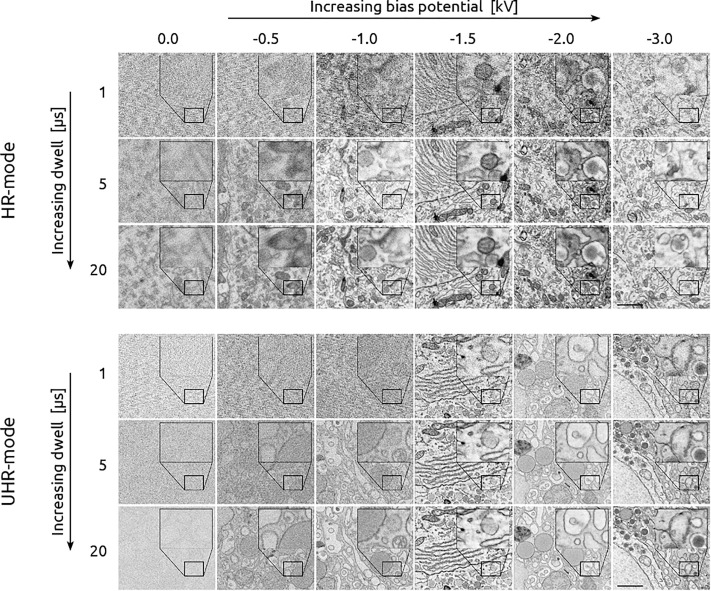
\includegraphics[width=\linewidth]{chapter-2/figures_JPEG_LQ/fig2-3_matrices.jpg}
    \caption{Negative bias potential delivers 5--20 times faster imaging while maintaining image quality. Bias potential varies from \SIrange[range-phrase=\text{ to }]{0}{-3}{\kilo\volt} (left to right) while the integration time varies from \SIrange[range-phrase=\text{ to }]{1}{20}{\micro\second} (top to bottom) for both the non-immersion (top) and immersion mode (bottom) image matrices. All images acquired with \SI{1.5}{\kilo\electronvolt} landing energy to match penetration depth. Scale bars: \SI{1}{\micro\meter}. Raw data is available at \href{www.nanotomy.org}{Nanotomy}.}
    \label{fig:2.3_matrices}
\end{figure}

An increase in image signal with increasing negative bias potential for both imaging modes up to roughly \SI{-1500}{\volt} was recorded (Figure \ref{fig:2.3_matrices}), after which it becomes difficult to perceive notable differences in image quality. The signal appears to improve more gradually in non-immersion mode, whereas the improvement for immersion mode is more abrupt. Furthermore, in certain instances, increasing the integration time by several factors results in a less substantial increase to the apparent SNR than a \SI{500}{\volt} increase to the negative bias potential. This is significant as the integration time is typically the primary imaging parameter to improve image quality—and large increases come at the direct expense of throughput.

Quantitative SNR measurements, based on the spectral signal-to-noise ratio (SSNR) \cite{unser1987new}, were made on the collection of images and averaged for each combination of bias potential, dwell, and imaging mode (Figure \ref{fig:2.4_snr}). These measurements were corroborated using a separate cross-correlation-based SNR method \cite{joy2002smart} (Figure \ref{fig:2.S2_comparison}). In particular, these measurements reveal that an image acquired in non-immersion mode with a \SI{1}{\micro\second} dwell time and \SI{-1.5}{\kilo\volt} bias potential yields roughly the same SNR as an image acquired with a \SI{5}{\micro\second} dwell but with no applied bias. The effect of the potential bias is even more pronounced in immersion mode where the SNR of a \SI{1}{\micro\second} image with a \SI{1.5}{\kilo\volt} stage bias exceeds that of a \SI{20}{\micro\second} image acquired without a bias. Fourier analysis was done to analyse the effect of the bias potential in different frequency domains (Figure \ref{fig:2.5_noise}). The center spot of the 2D FFTs—containing most of the signal—becomes more prominent with increasing bias potential. This growth is reflected in the SSNR spectra, which show order of magnitude increases in amplitude in the low spatial frequency domain. Furthermore, the high frequency streak artefacts present in the lower bias potential images---visible in the 2D FFTs---become suppressed at higher bias potentials.

% Figure 2.4 (SNR)
% ----------------
\begin{figure}[!tb]
    \centering
    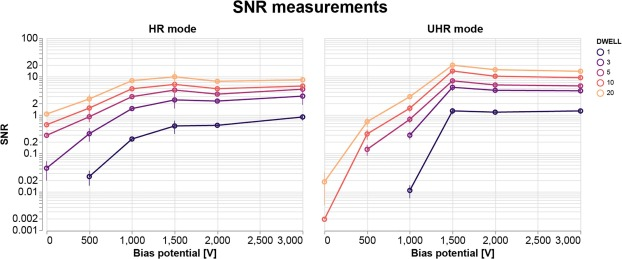
\includegraphics[width=\linewidth]{chapter-2/figures_JPEG_LQ/fig2-4_snr.jpg}
    \caption{Optimization of bias potential delivers SNR increases of multiple orders of magnitude. At bias potentials greater than \SI{1.5}{\kilo\volt}, the SNR is found to level off for both imaging modes. Images are comprised of varying stage bias potentials, integration times, and imaging modes but with fixed \SI{1.5}{\kilo\electronvolt} landing energy and \SI{5}{\milli\meter} working distance. Different color lines represent different dwell times as indicated by the legend. SNR measurements are averaged over five EM images at different areas of the tissue for each combination of bias potential, dwell time, and imaging mode. Error bars indicate the standard deviation in the SNR over the five images. Missing data points indicate a negative SNR, which may occur for images with extremely high noise.}
    \label{fig:2.4_snr}
\end{figure}


% Figure 2.5 (noise)
% ------------------
\begin{figure}[!tb]
    \centering
    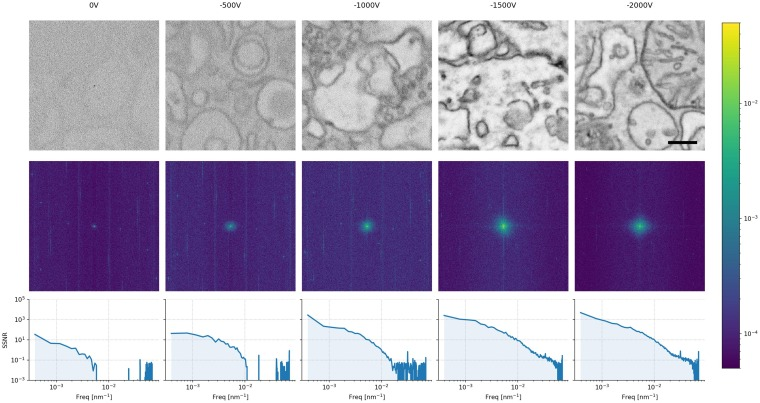
\includegraphics[width=\linewidth]{chapter-2/figures_JPEG_LQ/fig2-5_noise.jpg}
    \caption{Noise contributions suspected to originate from the scanning electronics are suppressed with increasing bias potential. Top: sequence of \SI{5}{\micro\second} dwell tissue images acquired in immersion mode with varying amounts of stage bias. Center: 2D FFTs of tissue images showing the central spot, which represents most of the signal, becoming more prominent with increasing bias potential up to \SI{-1.5}{\kilo\volt}. The 2D FFTs exhibit noticeable streak artefacts at higher frequencies, particularly in the lower bias potential images. We attribute these streaks to electric interference from the scanning electronics. Furthermore, there is a constant offset, which is likely a combination of shot noise from various sources, and may also include a component from the scanning electronics. Bottom: SSNR spectra show a division between the low frequency (primarily signal) and high frequency (primarily noise) portions of the tissue images. As the suspected scanning electronics noise is drowned out, the SNR improves dramatically. Scale bar: \SI{500}{\nano\meter}.}
    \label{fig:2.5_noise}
\end{figure}


% 2.2.4
% -----
\subsection{Potential bias allows for higher throughput EM and CLEM acquisitions}

Only small regions of interest are typically recorded at high resolution EM given that full section imaging at sub-\SI{10}{\nano\meter} resolution often takes an excessive amount of time. As a result of the enhanced signal-to-noise ratio afforded to us by the use of a negative bias potential, we are able to significantly expedite the imaging of a thin section of HeLa cells at \SI{5}{\nano\meter} resolution (Figure \ref{fig:2.6_cells}). Based on our empirical results (Figure \ref{fig:2.4_snr}), a negative potential bias of \SI{-1.5}{\kilo\volt} was chosen for EM imaging in immersion mode. A per-pixel dwell time of \SI{2}{\micro\second} was chosen to balance high SNR and image clarity with overall imaging time. Control images of the same cell were acquired without the use of a bias potential at the same landing energy (Figure \ref{fig:2.6_cells}A) and primary energy (Figure \ref{fig:2.6_cells}B). The total imaging time for this \SI{550}{\micro\meter} $\times$ \SI{350}{\micro\meter} area was \SI{5.6}{\hour}.

% Figure 2.6 (cells)
% ------------------
\begin{figure}[!tb]
    \centering
    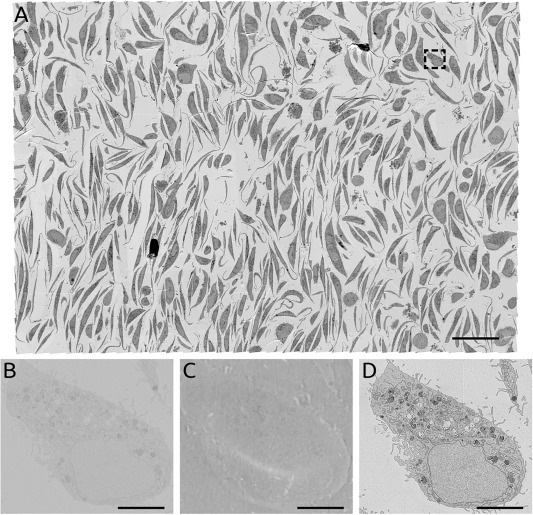
\includegraphics[width=\linewidth]{chapter-2/figures_JPEG_LQ/fig2-6_cells.jpg}
    \caption{Fast, high resolution EM gigapixel image of cultured cells. (A) EM acquisition of a \SI{100}{\nano\meter} section of HeLa cells as a nanotomy map. Section imaged at \SI{1.5}{\kilo\electronvolt} LE and with a \SI{-1.5}{\kilo\volt} bias potential. For the sake of comparison, one HeLa cell was acquired at multiple energy settings: (B) \SI{1.5}{\kilo\electronvolt} LE with no bias potential; (C) \SI{3}{\kilo\electronvolt} LE with no bias potential; (D) \SI{1.5}{\kilo\electronvolt} LE with \SI{-1.5}{\kilo\volt} bias potential—identical to that of the large-scale acquisition. Scale bars: \SI{50}{\micro\meter} (A); \SI{5}{\micro\meter} (B, C, \& D). Raw data is available for viewing via \href{www.nanotomy.org}{Nanotomy}.}
    \label{fig:2.6_cells}
\end{figure}

To demonstrate the application of a negative bias potential on samples also prepared for immunofluorescence, a large-scale acquisition was conducted on a section of rat pancreas tissue (Figure \ref{fig:2.7_rat}). Full section (\SI{0.5}{\milli\meter^2}) acquisition including fluorescence imaging, stage translations, and additional overhead factors was completed in \SI{8}{\hour}. Table \ref{tab:2.1_timing} provides an overview of the time spent on each aspect of the workflow, and exemplifies the potential time savings afforded by using a bias potential. We note that no post-staining was applied to this section in order to allow integrated acquisition of fluorescence for high-precision overlaid FM. Fluorescence images were acquired prior to EM to prevent quenching of the fluorescence due to electron beam irradiation. The insulin-producing beta cells---clustered within the islet of Langerhans---were immunolabelled and given a Hoechst counterstain to target cell nuclei as well as the rough endoplasmic reticulum in the exocrine region of the tissue (blue) (Figure \ref{fig:2.7_rat}A). The section edges can easily be discerned from the FM images, facilitating the area selection for subsequent EM imaging (Figure \ref{fig:2.7_rat}B). Here the islet (light grey region) can be seen surrounded by the exocrine tissue (dark grey). An automated registration procedure \cite{haring2017automated} was done to overlay the fluorescence signal onto the EM images (Figure \ref{fig:2.7_rat}C) such that the fluorescence signal is correlated at high resolution across the entire EM field of view (Figure \ref{fig:2.7_rat}D \& E). Additional details of how the correlative acquisition and reconstruction were done are provided in Sections \ref{sec:2.4.4_workflow} and \ref{sec:2.4.5_reconstruction} respectively.

% Figure 2.7 (rat)
% ----------------
\begin{figure}[!tb]
    \centering
    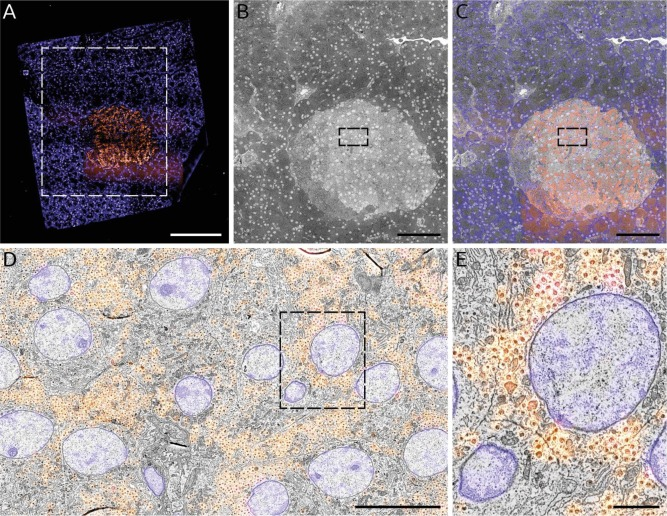
\includegraphics[width=\linewidth]{chapter-2/figures_JPEG_LQ/fig2-7_rat.jpg}
    \caption{Fast, correlative imaging of a complete EM section at high resolution. \SI{80}{\nano\meter} rat pancreas tissue was imaged at \SI{3}{\kilo\electronvolt} beam energy with a \SI{-1.5}{\kilo\volt} stage bias (\SI{1.5}{\kilo\electronvolt} landing energy) with \SI{2}{\micro\second} dwell as a nanotomy map. (A) Composite two-channel FM image of the tissue section: cell nuclei (blue) stained by Hoechst; insulin-producing beta cells (orange) immunolabeled with Alexa 594. (B) Composite EM image of the area outlined in (A) comprising the islet of Langerhans identified via FM imaging. (C) Correlative overlay of the islet and surrounding exocrine tissue. (D) Zoomed-in area of islet outlined in (B \& C) with inset (E) exhibiting the native resolution (\SI{5}{\nano\meter} pixel size) that exists across the entirety of the nanotomy map. Total imaging time is \SI{8}{\hour}, the majority of which is taken up by the high-resolution EM imaging. Note that a similar area at this pixel size (see e.g. \textcite{ravelli2013destruction}) typically takes upwards of \SI{24}{\hour} with TEM. Scale bars: \SI{200}{\micro\meter} (A); \SI{100}{\micro\meter} (B \& C); \SI{10}{\micro\meter} (D); \SI{2}{\micro\meter} (E). Raw data is available via \href{www.nanotomy.org}{Nanotomy}.}
    \label{fig:2.7_rat}
\end{figure}


% Table 2.1 (timing)
% ------------------
\begin{table}[!tb]
    \centering
    \caption{Use of optimized potential bias leads to an 80\% reduction in total imaging time for a typical large-scale acquisition. The total imaging time is highly dependent on the ROI size, which may vary widely depending on the biological application. Here the typical diameter of an islet of Langerhans is given, while in Figure \ref{fig:2.7_rat} a \SI{700}{\micro\meter} $\times$ \SI{700}{\micro\meter} area was chosen as the ROI—resulting in the \SI{8}{\hour} total acquisition time. Total imaging times for arbitrary ROI sizes can be determined by first calculating the number of image tiles needed: $N=\text{ceil}\left((L-ow) - (w-ow)\right)^2$ where $L$ is the typical section or ROI width, $o$ is the percentage overlap between image tiles, and $w$ is the field of view. Note that the negative overlap given for the low-magnification CLEM tiles reflects that these tiles do not overlap with one another.}
    \footnotesize
    \begin{tabular}{@{}p{15mm}p{30mm}rrrr@{}}
    \toprule
    \multicolumn{1}{r}{} & \multicolumn{1}{r}{} & \multicolumn{2}{c}{\textbf{Low-mag CLEM}} & \multicolumn{2}{c}{\textbf{Hi-mag EM}} \\
     \arrayrulecolor{black!30}\cmidrule(l){3-4} \cmidrule(l){5-6}
     &  & \textbf{No bias} & \textbf{Bias} & \textbf{No bias} & \textbf{Bias} \\
     \arrayrulecolor{black!30}\midrule
     & Pixel size & 36.6 nm &  & 4.88 nm &  \\
     & Dwell & 10 µs & 2 µs & 10 µs & 2 µs \\
     & Field of View & 150 µm &  & 20 µm &  \\
     & Overlap (b/w images) & −36 µm (−24\%) &  & 2.4 µm (12\%) &  \\
     & N. pixels & 16.8 Mpx &  & 16.8 Mpx &  \\
    \multirow{-6}{*}{EM} & Acquisition time & 168 s & 33.6 s & 168 s & 33.6 s \\
    \arrayrulecolor{black!30}\midrule
     & Exposure time & 5 s &  &  &  \\
     & N. channels & 2 &  &  &  \\
    \multirow{-3}{*}{FM} & Acquisition time & 10 s &  &  &  \\
    \arrayrulecolor{black!30}\midrule
     & Registration procedure & 20 s &  &  &  \\
    \multirow{-2}{*}{Overhead} & Stage translation & 4 s &  & 2 s &  \\
    \arrayrulecolor{black!30}\midrule
    Total & Total acquisition time (per CLEM/EM image) & 202 s & 68 s & 170 s & 36 s \\
    \arrayrulecolor{black}\midrule
    \rowcolor[HTML]{E8E8E8} 
    \cellcolor[HTML]{E8E8E8} & Typical size & 700 µm &  & 250 µm &  \\
    \rowcolor[HTML]{E8E8E8} 
    \cellcolor[HTML]{E8E8E8} & N. image tiles & 16 &  & 225 &  \\
    \rowcolor[HTML]{E8E8E8} 
    \multirow{-3}{=}{\cellcolor[HTML]{E8E8E8}Large-scale acquisition} & Total acquisition time & 54 min & 18 min & 11 hr & 133 min \\
    \bottomrule
    \end{tabular}
    \label{tab:2.1_timing}
\end{table}

\section{Discussion}
\label{sec:4.3_discussion}

We have demonstrated the ability of a CNN to artificially predict biological labels in electron microscopy images based on registered CLEM training data. This has important ramifications for many areas within cell biology in which additional labelling techniques are implemented to facilitate recognition of structures in EM \cite{de2015correlated}. In order to generate label predictions, registered EM-FM image pairs are required to train the CNN. Although in this work the accumulation of correlative datasets was facilitated by integrated CLEM, this is not a pre-requisite. Sequential CLEM methods in which light and electron microscopy are performed by different instruments in succession may also be suitable. It is unknown, however, what effects might come about from the use of fiducial markers and potentially less precise image registration across large fields of view.

While label predictions are not generalizable to arbitrary organelles outside of the training dataset, we have shown that the network is capable of transfer learning across cell types. Predictions on mouse breast tumor cell nuclei were made after supplementing a training dataset comprised primarily of rat pancreas tissue with a limited amount of correlative data from tumor cells. Aided by data augmentation, label predictions were furthermore found to be robust to changes in EM imaging parameters, additional shot noise, and sectioning artefacts. By further supplementing existing correlative datasets with data from different organisms, cell types, and microscopes, robustness could be improved even further.

The measured fluorescence and CLEMnet predicted labels fall short of providing adequate templates for fully automated segmentation. Nevertheless, we have shown that fluorescence labels are not only capable of facilitating annotation, but that as part of an image processing pipeline, they enable a framework for semi-automatic, weakly supervised segmentation. It is difficult to imagine that a deep CNN trained on automatically generated segmentation masks (i.e. no manual annotation whatsoever) could outperform the same network when trained on manually generated segmentation masks in the near future \cite{dorkenwald2017automated, januszewski2018high, roels2019domain}. Even so, semi-automated and fully automated approaches may still fulfill a role in segmenting biological image data. For smaller-scale applications in which training datasets are still tractable, a segmentation model based on manually segmented organelles is likely the more sensible approach. But for large-scale or volume applications in which a pixel-perfect segmentation may not be strictly necessary, a semi-automated labelling approach may offer valuable time-savings at the cost of precision.

The deep CNN developed here offers a means to do fluorescence-like labelling of electron microscopy data at negligible cost with respect to time, effort, and money. Once the network has been sufficiently trained, label predictions can be automatically generated in seconds. This would allow research facilities to process only a handful of sections for correlative fluorescence and electron microscopy, while preparing the rest of the sample for EM only. The entire EM volume could then be overlaid with fluorescence-like labels after training on the portion of the volume set aside for correlative imaging. In addition, EM datasets could be labelled with a larger number of distinct labels than would be allowed in a single fluorescence experiment by simply labelling different targets in different subsets of the sample.  Alternatively, it would enable comparative studies of multiple samples imaged by EM (e.g. \cite{sokol2015large, de2020large}) to be given biological labels virtually for free, providing biological insight to a wealth of grayscale data. 

\section{Methods}
\label{sec:4.4_methods}


% 4.4.1
% -----
\subsection{Tissue and sample preparation}
\label{sec:4methods_prep}

\subsubsection{Rat pancreas}
\label{sec:4methods_prep_rp}
Fresh pancreas from an 83 day old rat was cut into small pieces and fixed in 4\% paraformaldehyde (PFA, Merck) + 0.1\% glutaraldehyde (GA; Polysciences) as described in \textcite{ravelli2013destruction}. The sample was post-fixed in 1\% osmium tetroxide and 1.5\% potassium ferrocyanide in \SI{0.1}{M} cacodylate buffer, dehydrated through ethanol series and embedded in EPON (Serva). \SI{100}{\nano\meter} sections were cut and placed onto ITO-coated glass coverslips (Optics Balzers). Immunolabeling was performed as described previously \cite{kuipers2015scanning}. Samples were etched with 0.1\% periodic acid for 10 min, followed by a \SI{30}{\minute} blocking step: 1\% bovine serum albumin (BSA; Sanquin, Netherlands) in tris-buffered saline (TBS), pH 7.4. Next, anti-insulin was incubated for \SI{2}{\hour} (guinea pig; 1:50, Invitrogen, PA1-26938, RRID: AB\_794668) followed by washing and subsequent incubation for \SI{1}{\hour} with biotinylated secondary antibody (donkey-anti-guinea pig; 1:400, Jackson Immunoresearch) followed by washing steps. Finally, streptavidin conjugated AF594 (1:100, Jackson Immunoresearch) were incubated for \SI{1}{\hour} followed by washing a \SI{10}{\minute} incubation with Hoechst and washing.

\subsubsection{Mouse breast tumor cells}
\label{sec:4methods_prep_mbtc}
Mice were fixed by vascular perfusion with 4\% formaldehyde (FA) in \SI{0.1}{M} phosphate buffer (\SI{1.5}{\milli\liter\per\minute}) for ${\sim}$\SI{5}{\minute} until organs and eyes are clearly discolored. Tumors were dissected and cut immediately in blocks (${\sim}$\SI{1}{\milli\meter^3}) in 4\% FA fixative at room temperature. 4\% FA immersion fixation for \SI{3}{\hour} at room temp was continued with 2\% PFA + 2.5\% GA immersion fixation for \SI{2}{\hour} at room temperature, and the samples were stored in glass vials with 4\% FA until further processed. Samples were postfixed with 1\% osmium tetroxide and 1.5\% potassium ferrocyanide in \SI{0.065}{M} phosphate buffer for \SI{2}{\hour} at \SI{4}{\celsius} and finally for \SI{1}{\hour} with 0.5\% uranyl acetate. Dehydration was performed using a graded ethanol series. Samples were embedded in EPON resin (EMbed 812, EMS) and polymerized for \SIrange{48}{60}{\hour} at \SI{65}{\celsius}. Ultrathin section of \SI{100}{\nano\meter} were cut using a microtome (Leica, UC6) and placed on ITO glass. Hoechst 33258 (Sigma) staining was performed for \SI{120}{\minute} followed by a washing step with MilliQ water, and air dried.


% 4.4.2
% -----
\subsection{CLEMnet architecture}
\label{sec:4methods_architecture}

The design of CLEMnet (Figure \ref{fig:4M_architecture}) is based on U-net \cite{ronneberger2015u}, a deep CNN comprised of convolution, pooling, upsampling, and concatenation layers, designed for biomedical image segmentation. The U-net architecture was modified in several ways to make it more suitable for fluorescence predictions. The number of upsampling layers was reduced to address the resolution mismatch between EM and FM images. Additionally, the padding of images within convolution layers was removed to preserve image dimensions. Lastly, the number of convolution layers between each downsampling layer was reduced from two to one---roughly halving the number of parameters---to prevent overfitting \cite{balkenende2020clemnet}. The model architecture was developed in Tensorflow \cite{tensorflow2015-whitepaper}, an open source library for implementing machine learning models in Python, using the Keras API \cite{chollet2015keras}. All training and testing procedures were performed on NVIDIA Tesla P100 PCIe 12 GB GPU cards.

% --- Fig 4.M1 (architecture) ---
\begin{figure}[!tb]
    \centering
    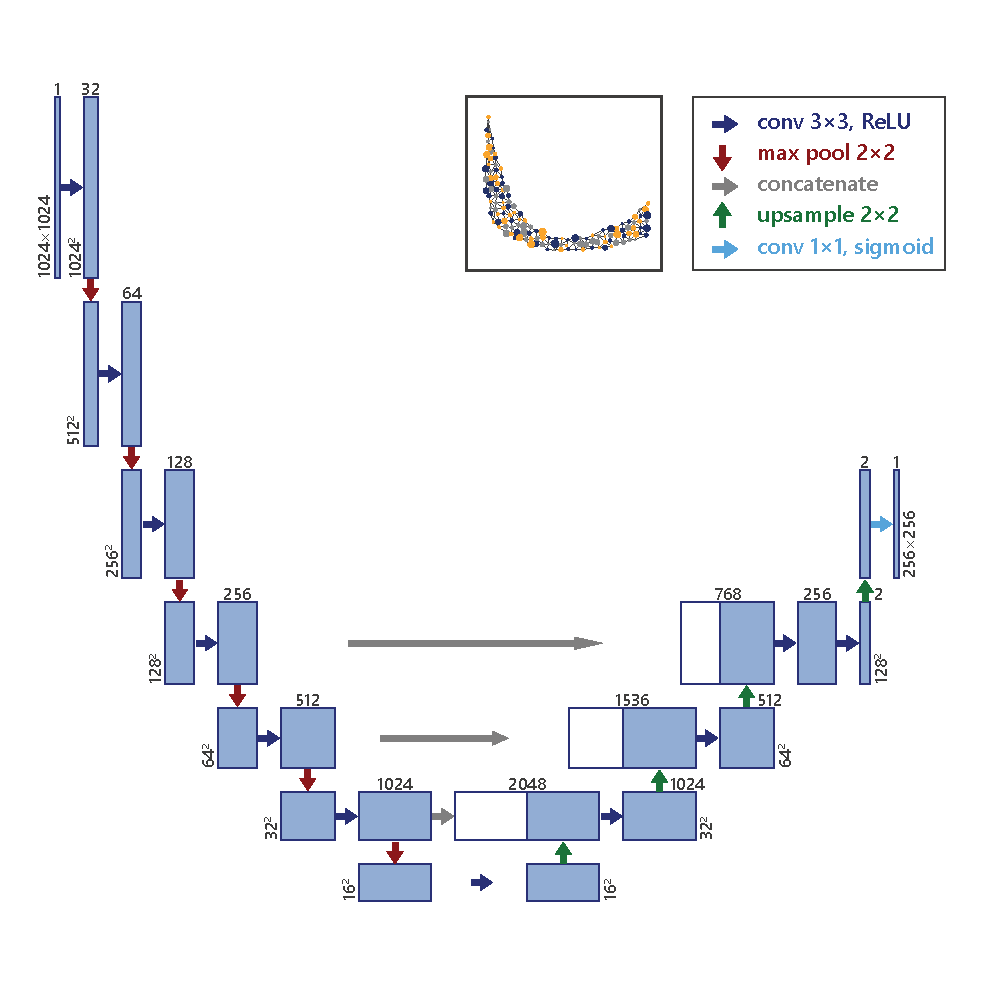
\includegraphics[width=0.95\linewidth]{chapter-4/figures_PDF/fig4-M1_architecture.pdf}
    \caption{CLEMnet architecture.
    The blue boxes correspond to multi-channel feature maps with the number of channels and image dimensions annotated above and to the side of each box, respectively. Arrows represent different possible operations as described in the legend. The asymmetric layout underlies the illustration from Figure \ref{fig:4.1_overview}B.}
    \label{fig:4M_architecture}
\end{figure}


% 4.4.3
% -----
\subsection{Data acquisition}
\label{sec:4methods_acquisition}
The integrated microscopy workflow for large-scale correlative imaging and reconstruction is described in \textcite{lane2021integrated}. Briefly, fluorescence imaging is done via the Delmic SECOM (Delmic B.V.), which has been retrofitted into the vacuum chamber of a Verios 460 SEM (Thermo Fisher Scientific) \cite{liv2013simultaneous, zonnevylle2013integration}. Correlative FM and low-magnification EM image tiles are acquired in a grid-like pattern encompassing each tissue section. The fluorescence is captured prior to EM to avoid quenching of the fluorescence. Following the acquisition of each correlative image pair, the FM tile is registered to the low-magnification EM tile by means of cathodoluminescent markers \cite{haring2017automated}. The fluorescence signal is then used to guide to regions of interest for subsequent, high-magnification EM, such as the islet of Langerhans in the case of the rat pancreas tissue. As thin sections of the mouse breast tumor cells are more or less homogeneous, acquisition areas were chosen based on minimal damage to the section. 

Each FM tile consists of a \SI{10}{\second} exposure at \SI{405}{\nano\meter} excitation for Hoechst and \SI{555}{\nano\meter} excitation for AF594. The corresponding low-magnification EM tiles are acquired at \SI{1.5}{\kilo\electronvolt} landing energy with a \SI{1}{\kilo\volt} bias potential, as described in \textcite{lane2021optimization}, with a \SI{400}{\pico\ampere} primary beam current, \SI{5}{\micro\second} dwell, and \SI{150}{\micro\meter} field width. The baseline imaging parameters for high magnification EM are the same as those for low-magnification EM with the exception of a \SI{2}{\micro\second} dwell and \SI{12}{\micro\meter} field width (${\sim}$\SI{3}{\nano\meter} pixel size). Imaging parameters for the datasets of mouse breast tumor cells acquired to assess network robustness are provided in Table \ref{tab:4M_params}. All of the image data used in this work is publicly available.\footnote{\href{https://sonic.tnw.tudelft.nl/catmaid/}{https://sonic.tnw.tudelft.nl/catmaid/}} Visualization and navigation of the large-scale datasets is made possible by CATMAID \cite{saalfeld2009catmaid}.

% --- Table 4.1 (params) ---
\begin{table}[tbh]
    \centering
    \caption{EM imaging settings used for the acquisition of resin-embedded mouse breast tumor cells. For data navigation purposes, Z index corresponds to section index within CATMAID.}
    \small
    \begin{tabular}
        {>{\raggedleft\arraybackslash}p{0.8cm} % Z
         >{\raggedleft\arraybackslash}p{2cm} % Section
         >{\raggedleft\arraybackslash}p{1cm} % LE
         >{\raggedleft\arraybackslash}p{1cm} % Dwell
         >{\raggedleft\arraybackslash}p{1cm} % PS
         >{\raggedleft\arraybackslash}p{1cm} % N
         >{\raggedleft\arraybackslash}p{1.5cm} % A
         >{\raggedleft\arraybackslash}p{1cm} % T
        }
        \toprule
        Z & Section ID & LE (eV) & Dwell (µs) & Pixelsize (nm) & N. EM images & Area\quad (µm × µm) & Time (hr) \\ 
        \midrule
        10--19 & S007A--S009C & 1500 & 2 & 3 & 484 & 234 × 234 & 4.5 \\
        0 & S002A & 1500 & 3 & 3 & 484 & 234 × 234 & 6.8 \\
        1 & S003B & 1500 & 1 & 3 & 484 & 234 × 234 & 2.3 \\
        2 & S003C & 1500 & 2 & 3 & 484 & 234 × 234 & 4.5 \\
        3 & S003D & 1500 & 2 & 4 & 289 & 241 × 241 & 2.7 \\
        4 & S004A & 1500 & 2 & 5 & 196 & 249 × 249 & 1.8 \\
        5 & S004B & 1500 & 2 & 6 & 121 & 235 × 235 & 1.1 \\
        6 & S005A & 1500 & 5 & 3 & 484 & 234 × 234 & 11.3 \\
        7 & S005B & 2000 & 2 & 3 & 484 & 234 × 234 & 4.5 \\
        8 & S006A & 1000 & 2 & 3 & 484 & 234 × 234 & 4.5 \\
        9 & S006B & 3000 & 2 & 3 & 484 & 234 × 234 & 4.5 \\
        \bottomrule
    \end{tabular}
    \label{tab:4M_params}
\end{table}


% 4.4.4
% -----
\subsection{Robustness \& validation}
\label{sec:4methods_robustness}
EM and FM image pairs are augmented during training to increase the robustness of the model. The objective is to improve the model's flexibility and to account for different types of imaging conditions rather than to extend it to different specimens. While the model may generate reasonable predictions of the fluorescence intensity on the same cell type or organelle across different specimens, it is not generalizable to tissue or cell types it has not been trained on. Several different types of data augmentation are applied to account for the variety of imaging settings the network would reasonably encounter if tested on EM data from other instruments.

% --- Affine transformation ---
\subsubsection{Affine transformation}
Affine transformations are applied to training data such that the model learns to adapt to modest changes in structural topology. By introducing minor adjustments to the rotation ($\theta$), translation ($t_x$, $t_y$), scale ($z_x$, $z_y$), and shear ($\Gamma$) of the training data, some degree of invariance to these transformations is embedded into the model \cite{simard2003best}. The applied affine transformations are randomized for each EM-FM image pair such that each image pair receives the exact same transformation (Figure \ref{fig:4M_affine}).

% --- Fig 4.M2 (affine) ---
\begin{figure}[!tbh]
    \centering
    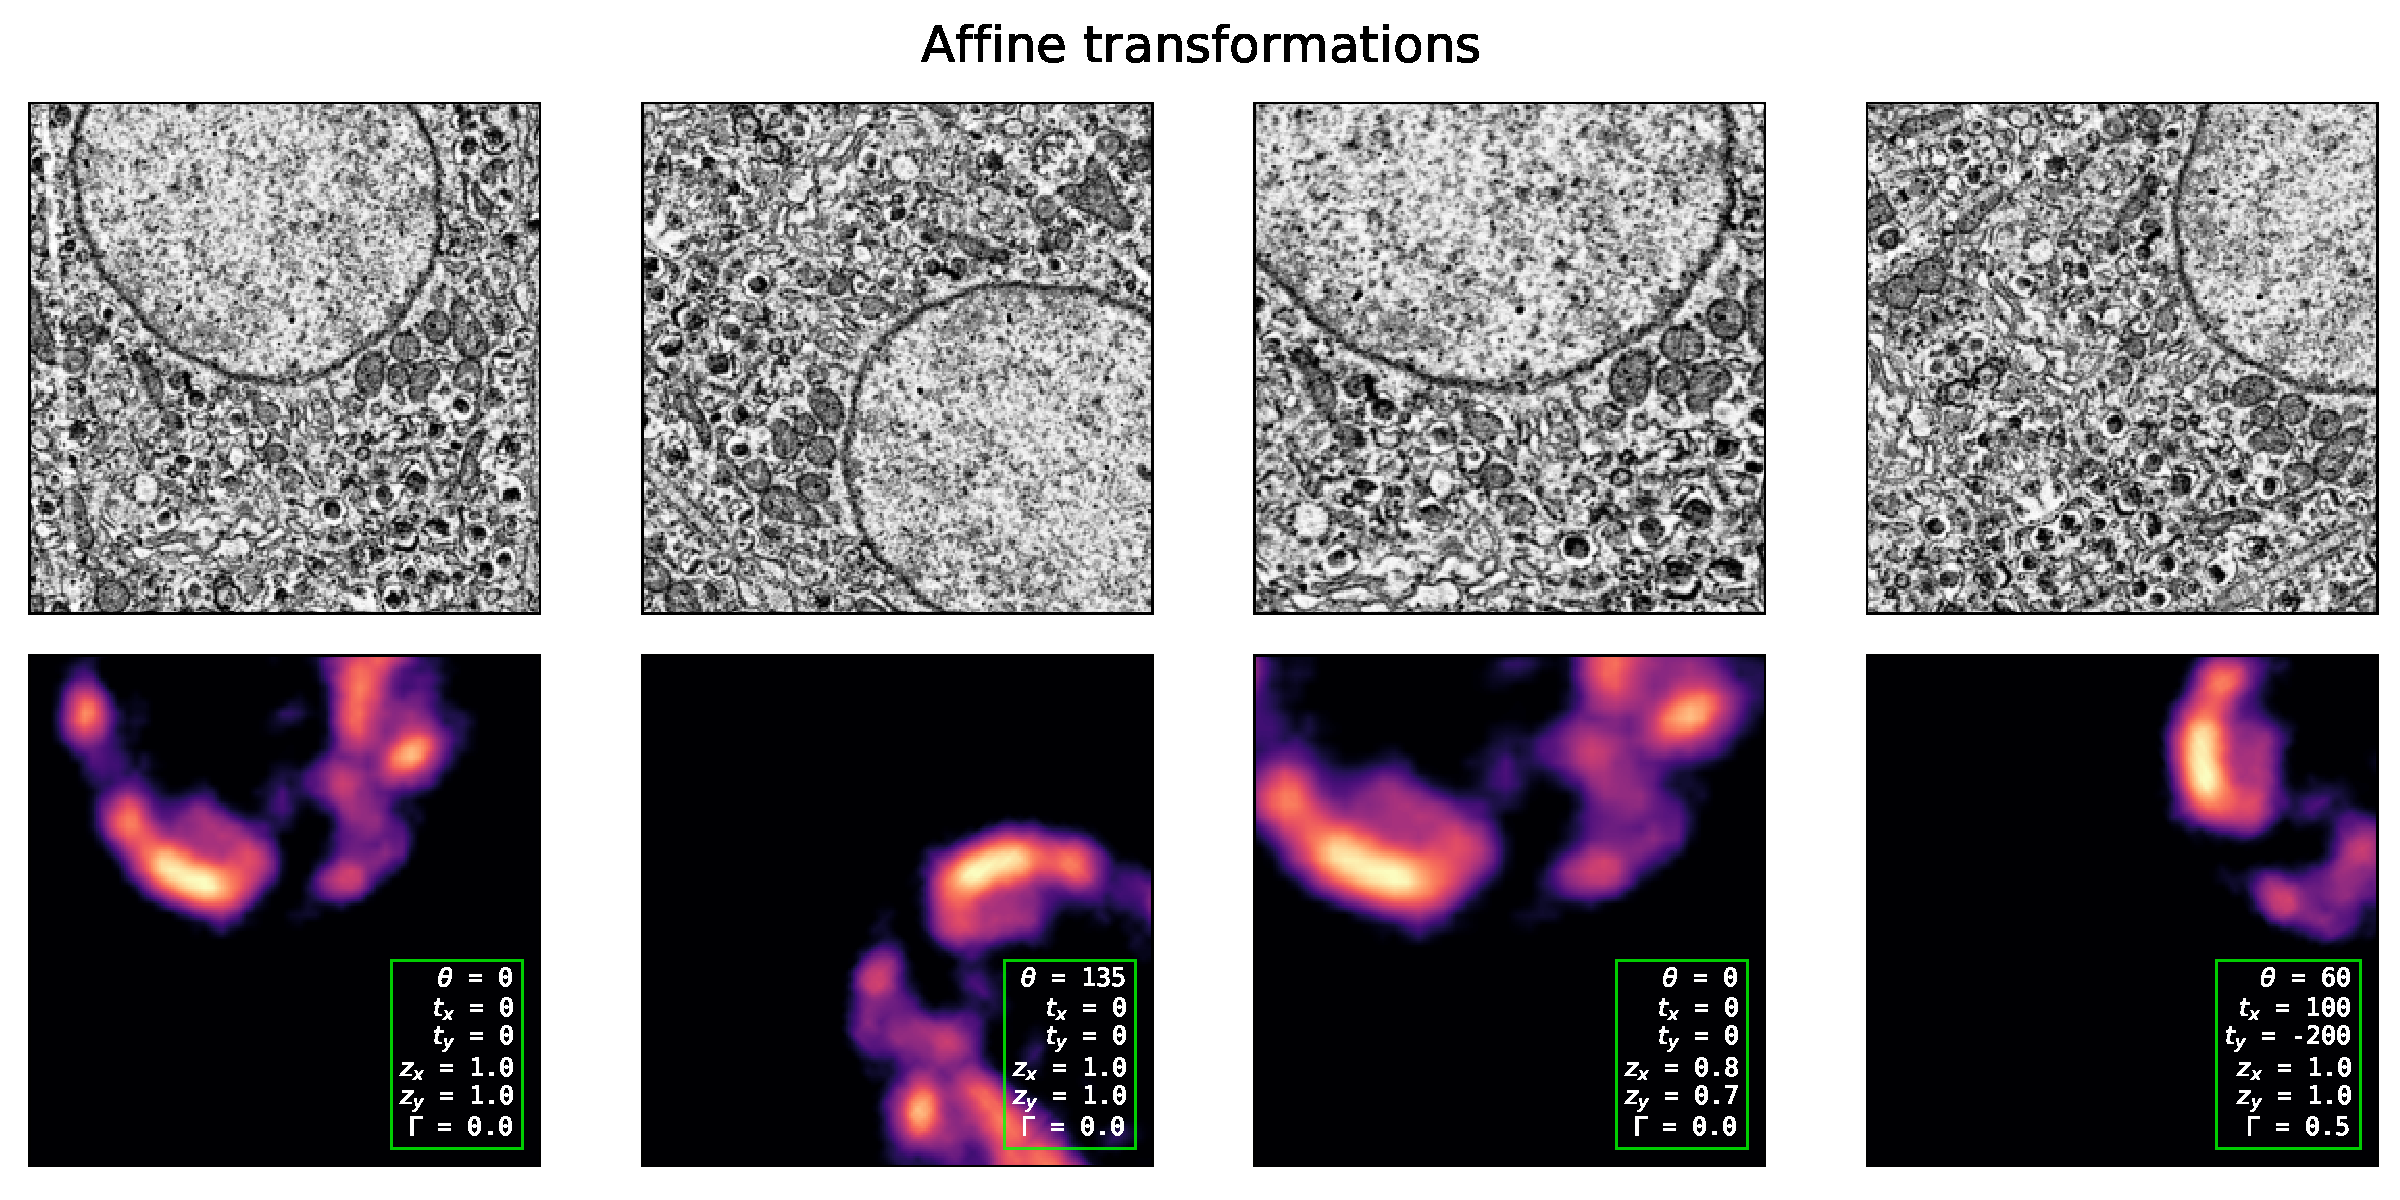
\includegraphics[width=\linewidth]{chapter-4/figures_PDF/fig4-M2_affine.pdf}
    \caption{Affine transformations are applied to the training data to render the model invariant to topological changes, resulting in greater robustness.
    The original, correlative image pair (left) may be rotated, translated, scaled, and sheared to encompass a wide variety of possible topological changes. Exact transformation parameters are provided in the text box of each transformed image pair.}
    \label{fig:4M_affine}
\end{figure}

% --- Elastic deformation ---
\subsubsection{Elastic deformation}
Elastic deformation was identified by \textcite{simard2003best} early in the development of neural networks as an effective means of augmenting training data. It was later shown by \textcite{dosovitskiy2014discriminative} and reinforced by \textcite{ronneberger2015u} as a crucial tool for enhancing CNN training, particularly in the case of limited training samples. Elastic deformations are generated by applying a non-linear warp to the image where the warp is defined by a displacement field convolved with a Gaussian kernel of standard deviation, $\sigma$, and multiplied by a scaling factor, $\alpha$ (Figure \ref{fig:4M_elastic}, top). The displacement field is initialized by a random uniform distribution where each pixel ranges from (-1, +1) with equal probability. The value for α is also randomized such that the EM images are warped with varying intensity. Distortions are more apparent along the edges of features (Figure \ref{fig:4M_elastic}, bottom).

% --- Fig 4.M3 (elastic) ---
\begin{figure}[!tb]
    \centering
    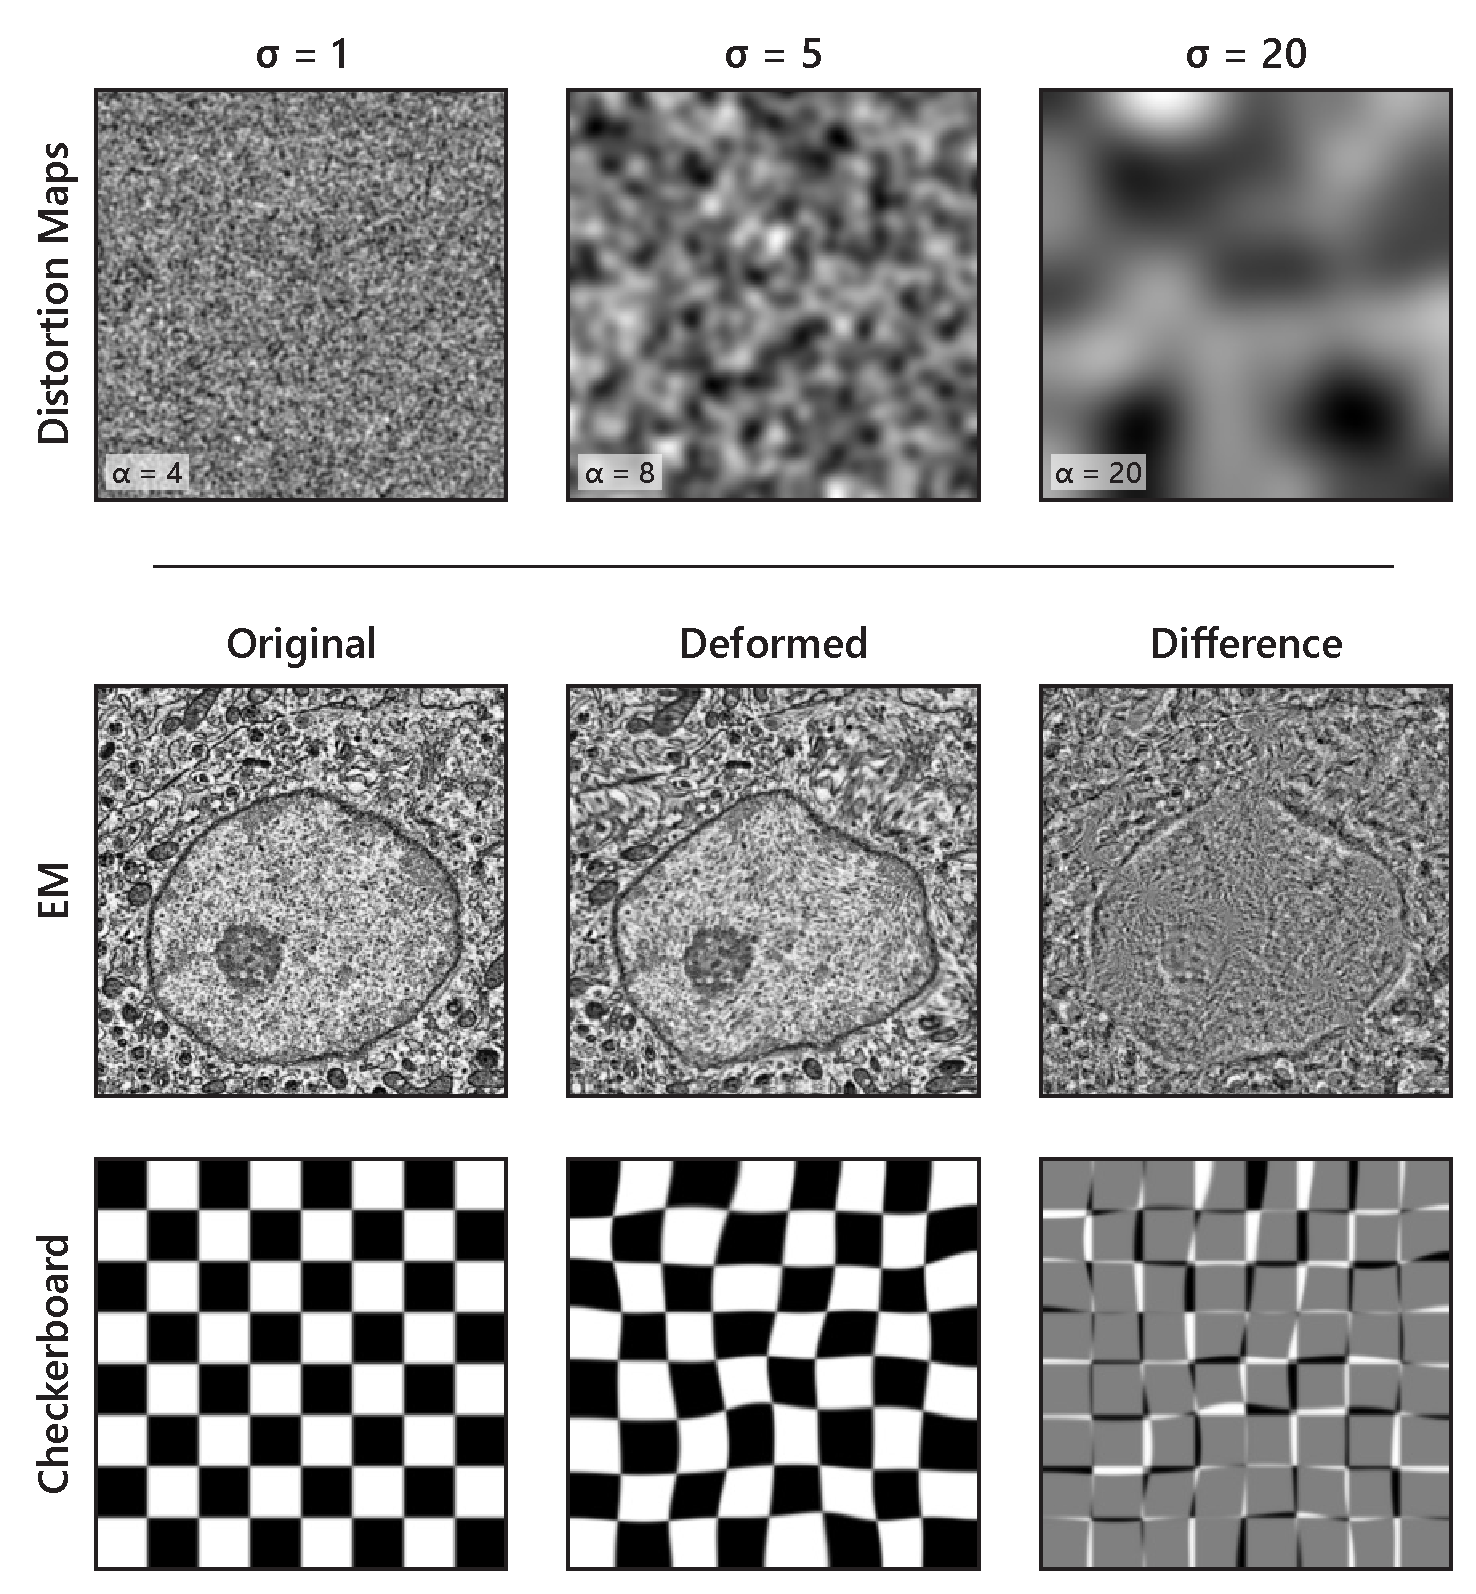
\includegraphics[width=\linewidth]{chapter-4/figures_PDF/fig4-M3_elastic.pdf}
    \caption{%
    Top: Distortion maps used for applying elastic deformations to training data. For small $\sigma$ the deformation resembles the addition of white noise, while for large $\sigma$ the deformation is more severe.
    Bottom: Elastic deformation applied to an EM training image and a checkerboard pattern.}
    \label{fig:4M_elastic}
\end{figure}

% --- Brightness / contrast ---
\subsubsection{Brightness \& contrast variation}
To account for the expected variations to brightness and contrast in EM image data acquired across different samples, microscopes, imaging settings, (day of the week), etc. the brightness and contrast levels are given a random adjustment. The brightness is varied ${\pm}$20\% by adding a gray-level bias, while the contrast is adjusted in the range $(0.75 < \delta < 1.5)$ where the value of each pixel, $x$, is scaled by
%
\begin{equation}
    (x - \bar{x})\,\delta + \bar{x}
\end{equation}
%
where $\bar{x}$ is the average intensity of the whole image.

% --- Noise augmentation ---
\subsubsection{Noise augmentation}
There are multiple sources of noise in the SEM detection chain, each with their own statistical distribution. The dominant source of noise on a properly operating SEM is, however, typically Poisson (shot noise) as additional contributions from the detector, scanning electronics, etc. tend to be much smaller than the statistical noise inherent in the signal \cite{joy2008noise}. Training images are therefore augmented with shot noise to improve the model’s robustness with respect to low SNR images (Figure \ref{fig:4M_noise}). The probability that a random variable $X$ is equal to $k$ is given by
%
\begin{equation}
    P(X=k;\lambda) = \frac{\lambda^{k} e^{-\lambda}}{k!}
\end{equation}
%
where $\lambda$ is the expectation value of $X$ as well as its variance.

% Fig 4.M4 (noise)
% ----------------
\begin{figure}[!tbh]
    \centering
    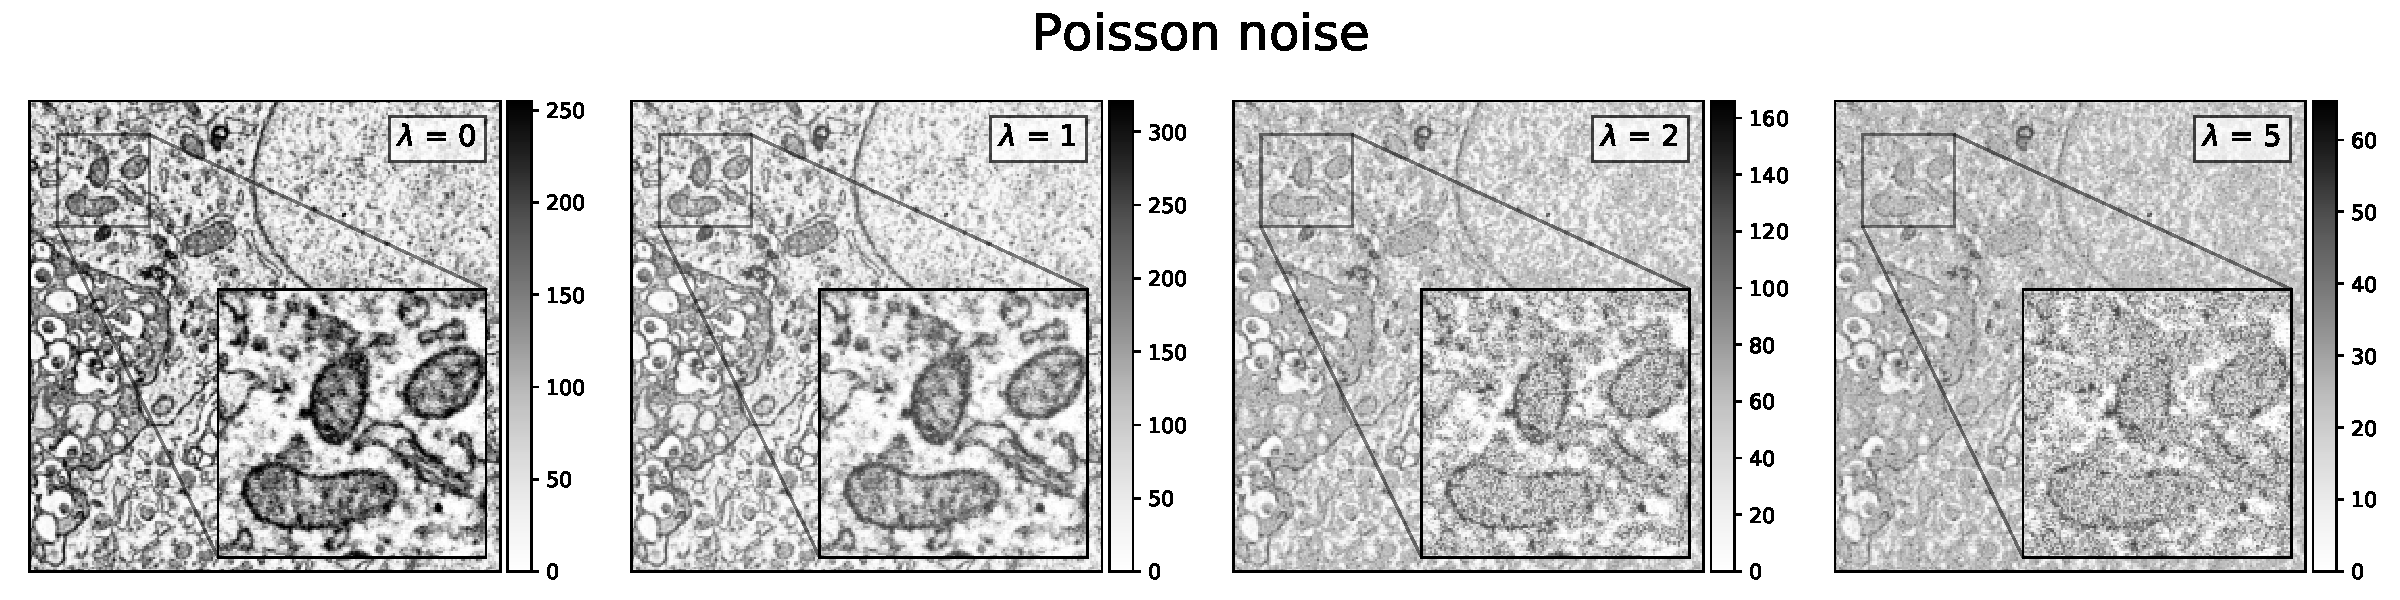
\includegraphics[width=\linewidth]{chapter-4/figures_PDF/fig4-M4_noise.pdf}
    \caption{Poisson noise added to an EM training image.
    Features become unrecognizable at high values of $\lambda$.}
    \label{fig:4M_noise}
\end{figure}


% 4.4.5
% -----
\subsection{Quantitative analysis}
\label{sec:4methods_analysis}

\subsubsection{Cell nuclei counting}
Experts and trained volunteers were asked to recognize cell nuclei in datasets comprised of fluorescence signals obtained with a microscope and generated by CLEMnet. The experts consisted of two researchers from the University Medical Center Groningen who routinely examine islets of Langerhans, while the volunteers consisted of thirteen researchers from within the TU Delft Department of Imaging Physics who were trained to recognize cell nuclei in both FM and EM image data from comparable tissue. The annotations made by the experts were weighted by a factor 3.

An unsupervised, brute-force nearest neighbors search was used to filter outlier annotations from the EM dataset. For each annotated point, the Euclidean distance to every other annotated point was calculated. If a point was found to have at least 12 neighboring points (corresponding to ${\ge}$80\% of annotators) within a radius roughly equal to the average radius of a cell nucleus, the point was kept. Points with an insufficient amount of neighboring points were discarded, resulting in clusters of point clouds corresponding to the ground truth nuclei. $k$-means clustering was then used to agglomerate point clouds from which the centroid of each cluster could be computed and added to the ground truth set.

\subsubsection{Segmentation evaluation}
Segmentation performance is evaluated by the intersection over union (IoU), a similarity coefficient used to measure the overlap of two sets $A$ and $B$.
%
\begin{equation}
    IoU(A, B) = \frac{\left|\,A \cap B\,\right|}{\left|\,A \cup B\,\right|}
\end{equation}



% 4.4.6
% -----
\subsection{Segmentation}
\label{sec:4methods_segmentation}

\subsubsection{Fully supervised segmentation}

Segmentation masks for training were generated either by manually tracing cell nuclei in EM images of rat pancreas islets (using GIMP) or by thresholding the measured fluorescence or CLEMnet prediction images. A value of 0.2 was empirically chosen to be the threshold after rescaling the intensity range from (0, 255) to (0, 1). To reduce the burden on manual tracing, a higher zoom level was chosen than for generating fluorescence predictions. 96 images from across six different sections were manually segmented. One section was set aside for testing, while the five remaining sections were divided 80\%/20\% for training and validation. Implementation of the ResNet-34 model architecture was facilitated by Segmentation Models \cite{Yakubovskiy:2019}, which provides neural network frameworks for image segmentation compatible with Keras and Tensorflow.


\subsubsection{Partial points annotation}

Labelled images are generated in a two-phase process adapted from \textcite{qu2020weakly}. In the first phase (Figure \ref{fig:5M_segmentation}A), partial points annotation is used to generate a probability map for the location of cell nuclei. Partial points annotation was performed on the same dataset as used for the fully supervised segmentation. Though all nuclei visible in the EM were annotated, only five were chosen at random for generating Gaussian masks (PP Mask). The values for the Gaussian masks are given by
%
\begin{equation}
    M_i = 
    \begin{cases}
        \text{exp}\left({-\frac{D_i^2}{2\sigma^2}}\right) & \text{if}\; D_i < r_1, \\
        0 & \text{if}\; r_1 < D_i < r_2, \\
        -1 & \text{otherwise}
    \end{cases}
\end{equation}
%
where $D_i$ is the radial distance from each pixel $i$ to the nearest partial point, $\sigma$ is the standard deviation of the Gaussian distribution over each partial point, and $r_1$ and $r_2$ are the typical nuclear radius (estimated from the validation dataset) and the outer radius of background labels, respectively. Here we have used $r_1=\text{\SI{5}{\micro\meter}}$, $r_2 = 2 r_1$, and $\sigma = r_1 / 2$. In this way each pixel is classified as either nucleus ($>\text{0}$), background (0), or remains unlabelled ($-\text{1}$).

When trained on pairs of EM images and PP masks, ResNet-34 yields probability maps of predicted nuclei locations for given input EM test images. The initial probability map, though rather crude, is used to refine the PP mask to generate a better estimate of the background. The background estimate is updated according to the conditions
%
\begin{equation}
    M^N_i = 
    \begin{cases}
        M_i & \text{if}\; D_i < r_2, \\
        0 & \text{if}\; D_i > r_2 \quad \text{and} \quad p_i < 0.1, \\
        -1 & \text{otherwise}
    \end{cases}
\end{equation}
%
where $p_i$ is the probability of that pixel belonging to the nucleus class after iteration $N$. The pipeline is designed in such a way to as to iteratively yield better and better probability maps. We find, however, that the maps tend to converge after $N=\text{2}$ for this particular dataset.

% Fig 4.M5 (segmentation)
% -----------------------
\begin{figure}[!tb]
    \centering
    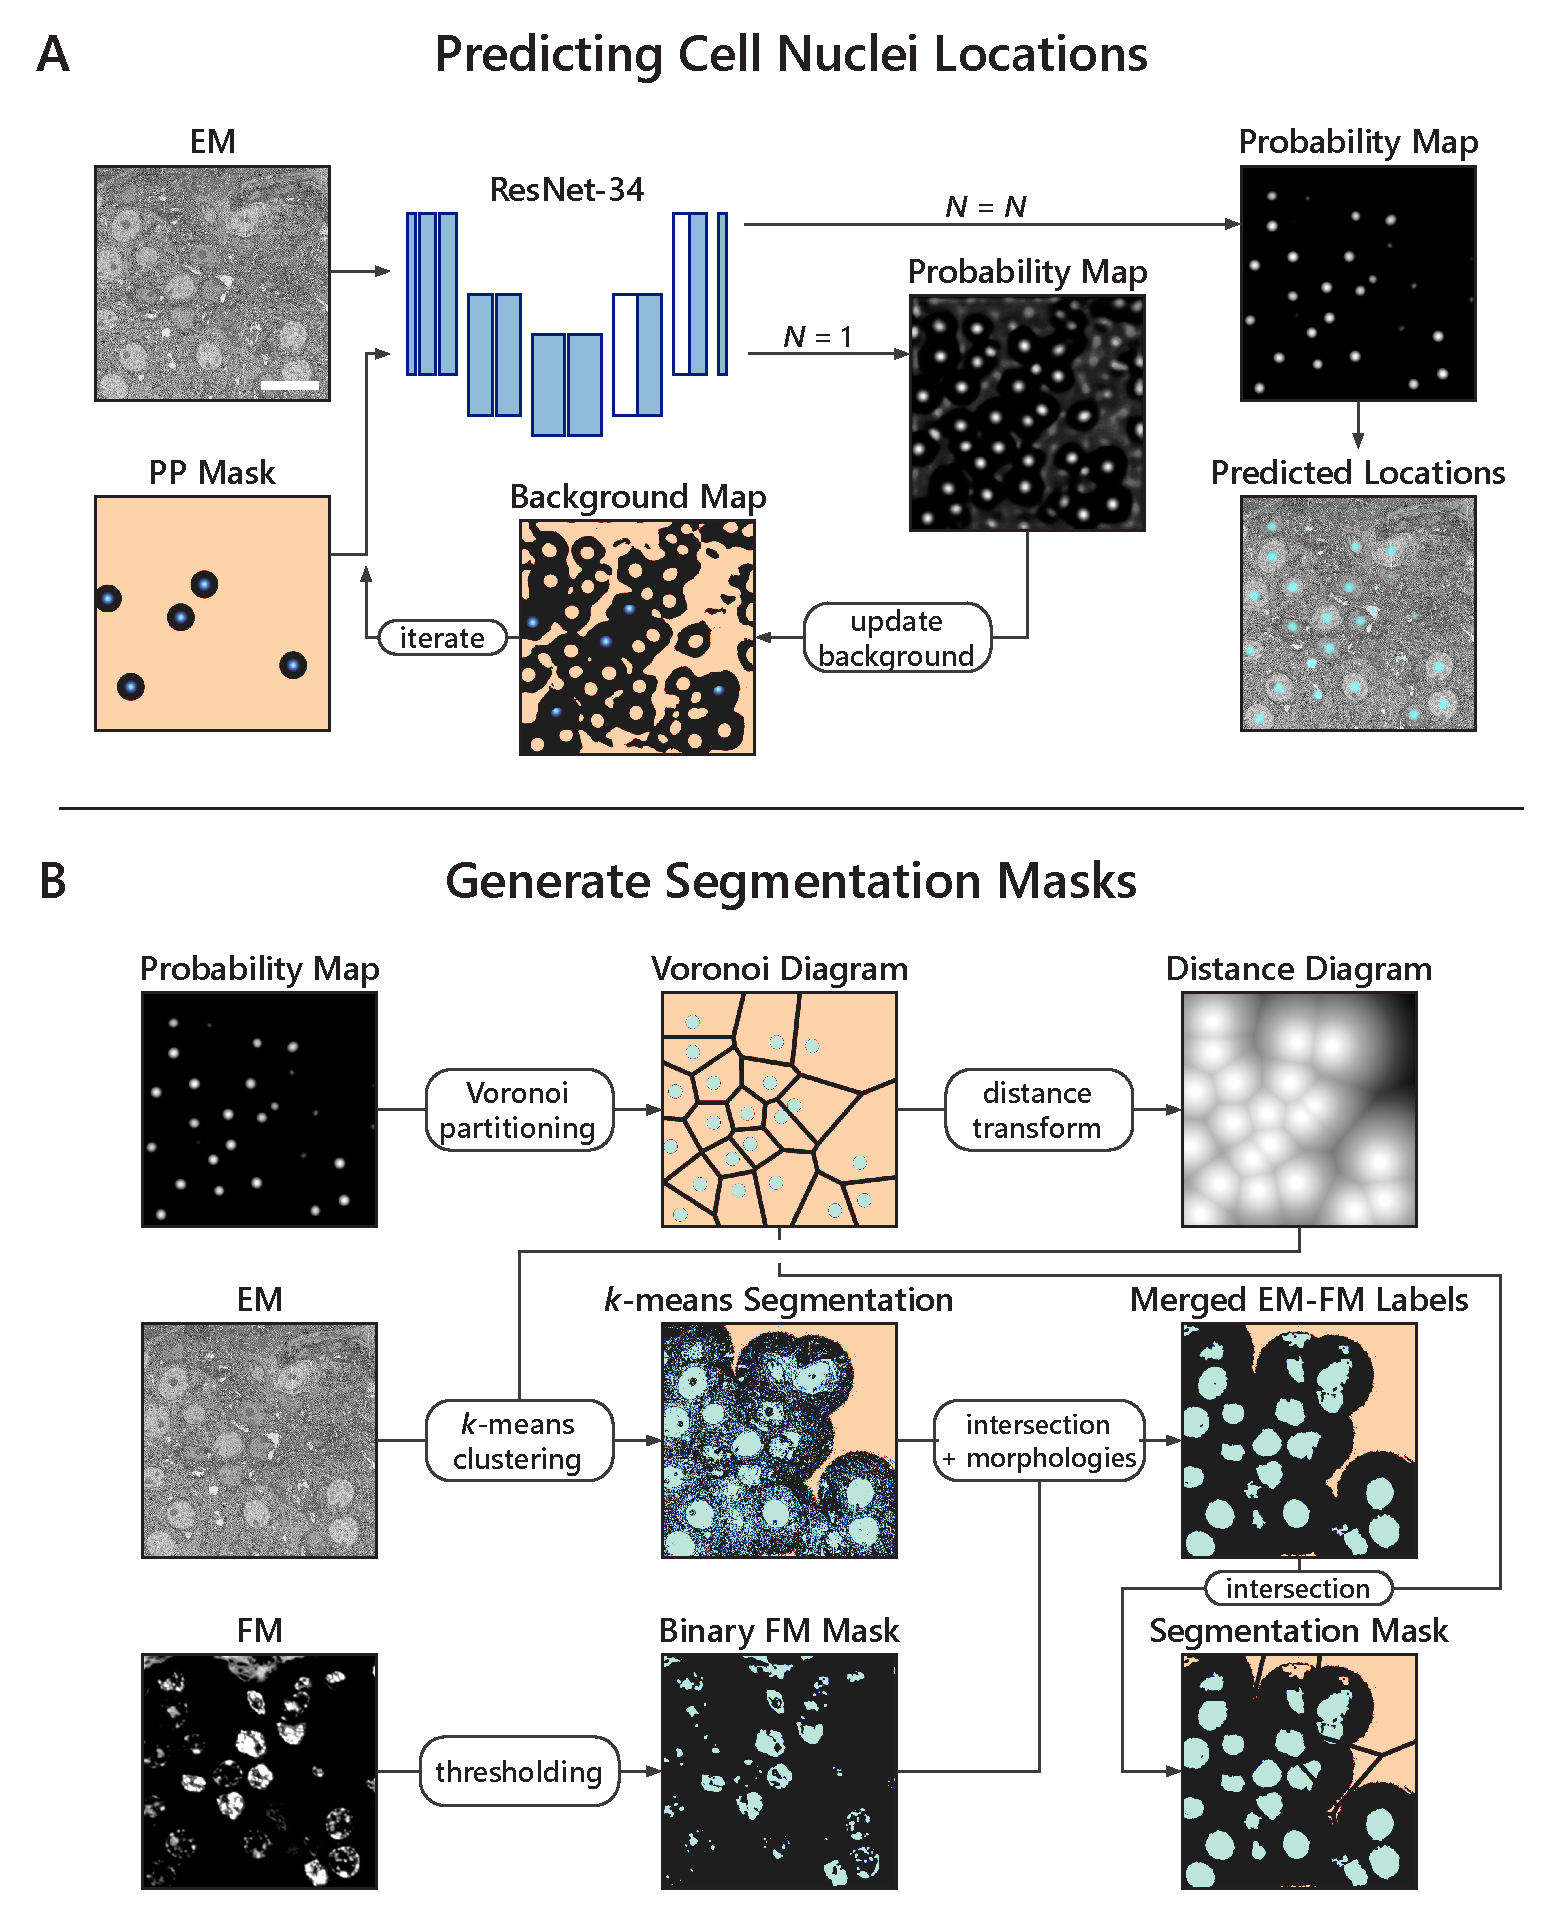
\includegraphics[width=0.90\linewidth]{chapter-4/figures_PDF/fig4-M5_segmentation.pdf}
    \caption{Semi-automated image processing pipeline for generation of segmentation masks from partial points annotation.
    (A) Partial points annotation is used to create Gaussian mask images to train an instance of ResNet-34 to predict nuclei locations. The predictions are refined through self-training to yield more accurate probability masks.
    (B) A Voronoi diagram based off of the probability map in (A) is merged with labelled images from $k$-means clustering to create segmentation masks for training a separate instance of ResNet-34 for organelle segmentation.
    Legend: white (or cyan) -- nucleus; black -- background; beige -- unlabelled.
    Scale bar: \SI{10}{\micro\meter}.}
    \label{fig:5M_segmentation}
\end{figure}

In phase two (Figure \ref{fig:5M_segmentation}B), segmentation masks are generated by a combination of $k$-means clustering and a Voronoi partitioning of the nuclei detected in phase one. These two labelling schemes are complementary to one another. $k$-means clustering preserves the spatial information in the EM image, providing the contour of the nuclei at the expense of having greater uncertainty, while the Voronoi partition provides accurate nuclei localization at the expense of underestimating the background label. The EM image is multiplied by the distance transform of the Voronoi diagram prior to $k$-means clustering to amplify nuclei. Clustering is then done with $k=\text{3}$. We choose to subtract a value of 1 from the resulting image such that the background goes to $-\text{1}$ (unlabelled). In this way the model does not train on regions of the image where a label cannot easily be inferred from either the $k$-means clustering or Voronoi partitioning. These regions are typically in the void between adjacent nuclei where it can be disadvantageous to make an assumption on whether a pixel belongs to the nucleus or background class, as it is possible that a nucleus was missed in phase one.

The fluorescence image is independently thresholded and intersected with the $k$-means clustered image. Small segments are removed via morphological opening, closing, and erosion operations. Larger segments are filtered by convexity, measured as the ratio of the area of each segment relative to the area of its convex hull. Segments with convexity less than 0.85 become unlabelled. Lastly, the merged labels from $k$-means clustering of the EM and thresholding of the FM are intersected with the Voronoi diagram to result in a final segmentation mask. Pairs of segmentation masks and EM images are then used to train an instance of ResNet-34 for organelle segmentation in the same manner as was described for fully supervised segmentation. Note that the fluorescence image was originally included as a separate channel during $k$-means clustering, but the results from doing so were marginally worse: final IoU score of 67\% vs 72\%.

\clearpage
\section{Supplementary material}
\label{sec:4_supplement}
\renewcommand{\thefigure}{S\arabic{figure}}
\setcounter{figure}{0}    

% Figure 4.S1 (ROIS)
% ------------------
\begin{figure}[!tbh]
    \centering
    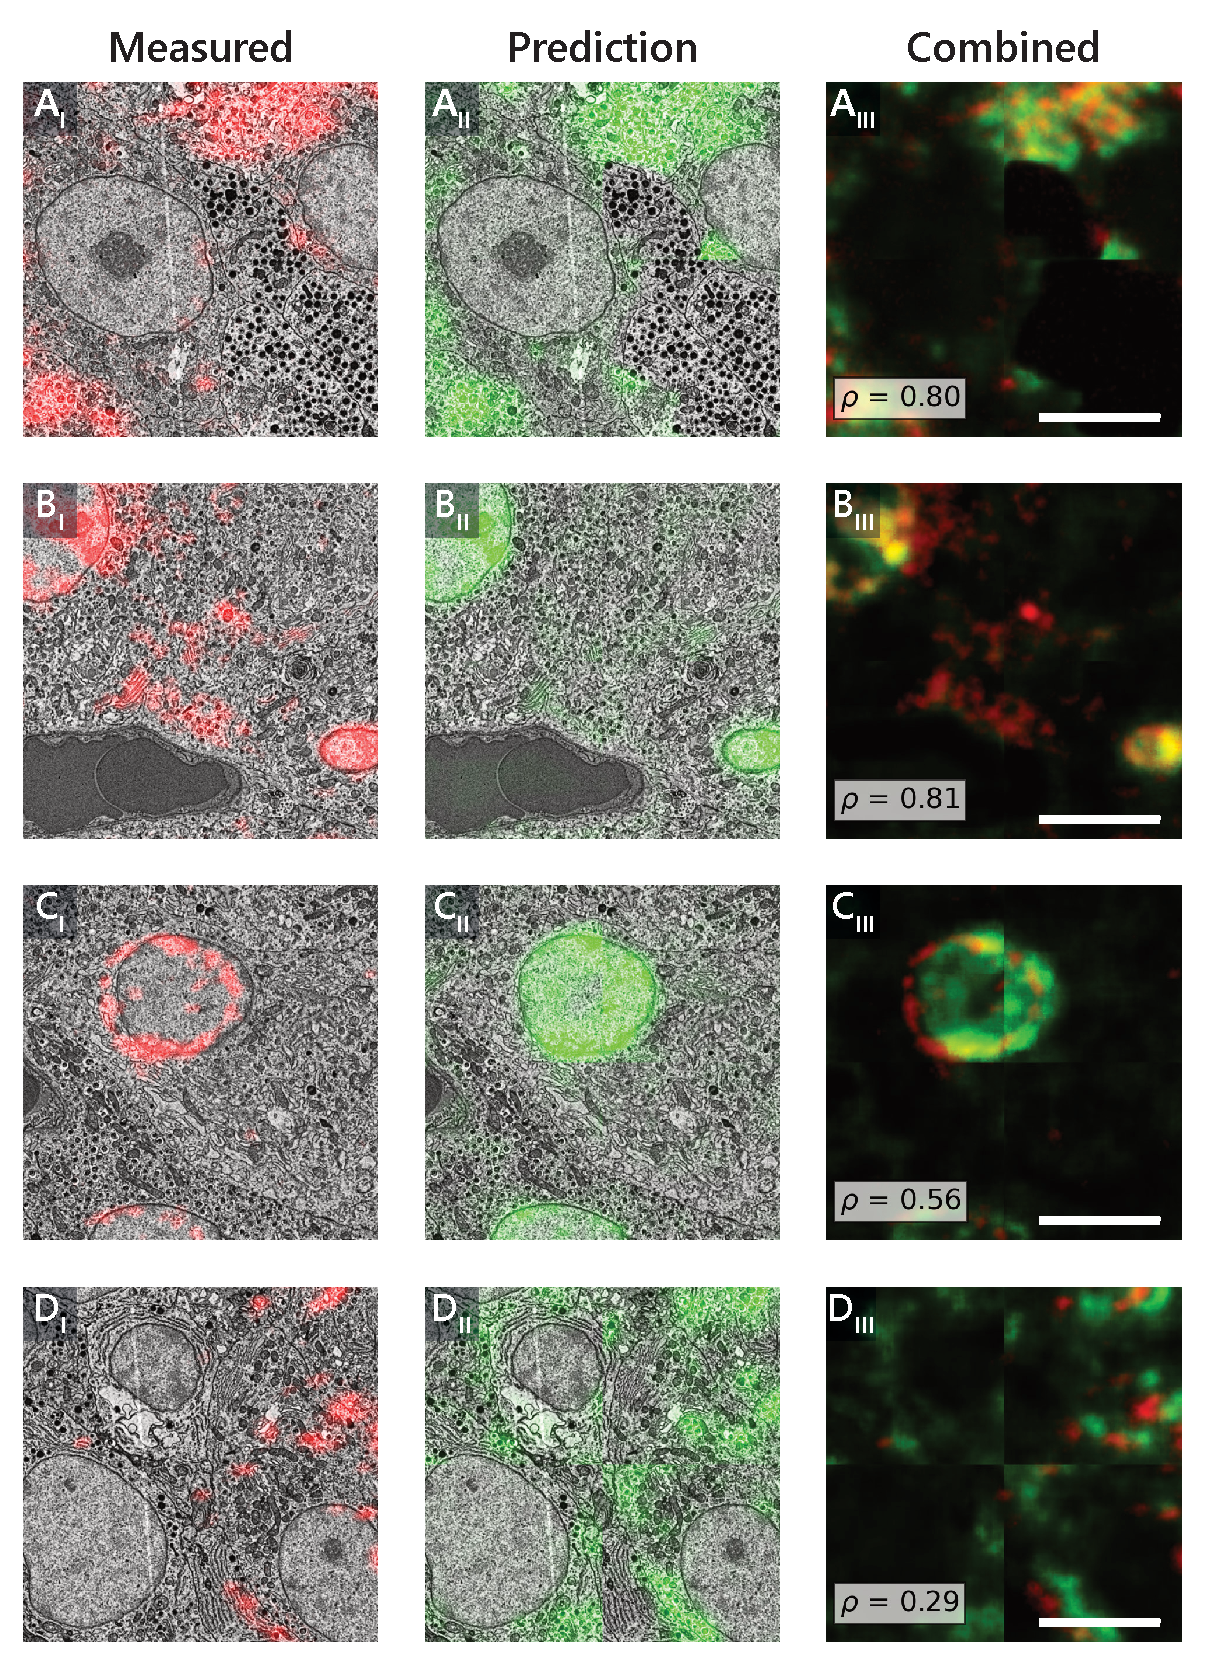
\includegraphics[width=0.95\linewidth]{chapter-4/figures_PDF/fig4-S1_rois.pdf}
    \caption{CLEMnet is able to perform nontrivial structural recognition tasks as well as mitigate issues inherent to fluorescence imaging. (Continued on next page\ldots)}
    \label{fig:4.S1_rois}
\end{figure}
\addtocounter{figure}{-1}
\begin{figure}
    \caption{For each selected ROI (A-D), the measured fluorescence (left, red) and prediction (center, green) are overlaid onto the EM, and combined to show overlap and differences in signal intensity (right).
    (A) The network is able to distinguish between insulin and similar-looking glucagon granules, a difficult task for non-experts.
    (B) An instance of AF594 emission from \SI{405}{\nano\meter} Hoechst excitation demonstrates that the network prediction is less susceptible to bleedthrough. 
    (C) As the network generates predictions directly on structures within the EM, it is able to compensate for errors in the EM-FM registration near the edges of the field of view where the registration may be extrapolated.
    (D) The network is for the same reason also less susceptible to off-axis aberrations such as vignetting, which results in diminished signal at the corners of the fluorescence field of view.
    Note that several predictions are stitched together to compose the predicted image shown, at times giving rise to edge artefacts.
    Scale bars: (A--D) \SI{5}{\micro\meter}.}
\end{figure}

\quad


% TODO:
%  finalize in preparation statement
%  check for all instances of HeLa cells --> should be tumor cells
%  abstract
%  methods section for segmentation
%  add references

% References
\printbibliography[title={References}]
  % CLEMnet
% \chapter{Conclusion}
\label{chap:5}
\begin{refsection}

% % Abstract
% \section*{Abstract}
% \begin{small}
%     abstract
% \end{small}

\section{Valorisation}
\label{sec:5.1_valorisation}

This thesis presents a novel workflow for three-dimensional correlative light and electron microscopy (3D CLEM) in the form of integrated array tomography. The method involves correlative imaging of and volume reconstruction from serial sections of biological tissue using an integrated fluorescence and electron microscope. Integrated array tomography offers several advantages over alternative approaches for 3D CLEM.

% \setlist{nolistsep}
\begin{enumerate}[label=(\Roman*)]
    \item Semi-automated imaging and fully-automated registration facilitate the correlative acquisition of large numbers of serial sections. We have demonstrated the scalability of our method to 64 sections of zebrafish pancreas in which the only limitation was on the number of serial sections that were prepared (Chapter \ref{chap:3}). Additionally, the correlative reconstruction routine supports the alignment of an arbitrarily large number of sections.
    \item \textit{In-situ} targeting of ROIs expedites throughput by limiting imaging volumes to those regions expressed by fluorescence. In practice we have experienced tenfold decreases to the imaging volume with corresponding reductions to acquisition times and dataset sizes (Chapter \ref{chap:3}).
    \item Because the specimen is simultaneously prepared for both FM and EM, the reconstructed volumes of correlative data have matching axial resolution. This means that the fluorescence data does not have to be projected or interpolated in $z$ as is the case with certain sequential CLEM approaches. Furthermore, specimen warping and shrinkage, which might otherwise occur in conventional array tomography methods, is prevented due to the absence of intermediate sample preparation.
    \item Precise overlay of biological molecules and structural context at high resolution is achievable in all three dimensions. We have demonstrated sub-\SI{100}{\nano\meter} typical overlay accuracy and worst-case-scenario misalignment of ${\sim}$\SI{1}{\micro\meter} (Chapter \ref{chap:3}).
    \item Array tomography allows for re-evaluation of sections, if necessary, as opposed to serial blockface (SBF-SEM) or focused ion beam (FIB-SEM) techniques in which the specimen is destroyed as it is imaged.
\end{enumerate}

While the method has its advantages, it is not, of course, without its limitations. Chief among them is the manual intervention needed for certain navigation and focusing tasks. Although the ability to detect regions of interest on-the-fly based on fluorescence is one of the main benefits of integrated array tomography, these regions must still be navigated to manually. To further automate the workflow, ROI positions for each section could be extrapolated based on an initial selection, as in \textcite{gabarre2021workflow}. Slight variations in section shape can be accounted for by a geometrical transformation of each serial section to the reference section from which the ROI was initially selected. An alternative approach for fully automated ROI detection and navigation involves recognition of the fluorescent markers of interest based on artificial intelligence (AI). \textcite{delpiano2018automated} investigated this approach for the automated detection of fluorescent cells, finding that current state-of-the-art machine learning techniques required significant quantities of ground truth training data as well as postprocessing for separating merged cells. Thus, while fully automated AI-based approaches for ROI detection may not yet be suitable, opportunities for extending automated navigation do exist.

The other component of the workflow that stands to benefit most from automation are the EM and FM focusing routines. Effort has been invested in developing an autofocus procedure for the fluorescence microscope (Appendix \ref{app:A}), which involved analyzing the performance of several dozen focus metrics. The results were ultimately incorporated into the autofocus routine implemented in the integrated microscope control software, Odemis. Developing an EM autofocus routine has been a more complex task as it requires access to proprietary software for controlling the lens voltages. With the development of FAST-EM \cite{fermie2021high}, access to these controls has become available through an extension to Odemis. The potential for fully automated focus routines is therefore in place, however, questions surrounding the robustness of these routines remain. Therefore, the choice was made to forgo autofocusing routines during large-scale acquisitions to prevent the possibility of a failure compromising subsequent acquisitions.

Challenges pertaining to sample preparation were described in Section \ref{sec:3.4_discussion}. In short, fluorescent probes, such as fluorescent proteins, are generally incompatible with conventional fixation and staining procedures used for EM. Despite efforts towards developing probes for retaining fluorescence post-embedding \cite{watanabe2011protein, kukulski2011correlated, peddie2014correlative}, compromises between the strength of the fluorescence and the quality of the ultrastructure remain unavoidable. These compromises are made more difficult by conducting fluorescence imaging in high vacuum conditions where intensities are expected to be lower as fluorescent probes are typically optimized for (if not dependent on) aqueous environments \cite{peddie2014correlative}.

Finally, fluorescence preservation or post-embedding relabeling of genetic fluorophores may facilitate linking ultrastructural observations to live, intravital fluorescence microscopy. Prior to array tomography, photoactivatable probes could be used to mark where cells can be assessed for function. These markers could then be activated as part of the integrated workflow, thus linking the ultrastructural data to not only fluorescence expression but also to function and development \cite{collinson2017correlating}. If combined with advances in automation, this could lead towards the development of dedicated integrated CLEM instruments with complete and fully automated workflows for high-throughput and high-yield volume CLEM.

\section{Applications for multibeam SEM}
\label{sec:5.2_mbsem}

For certain applications such as connectomics, in which the goal is to comprehensively reconstruct neuronal circuitry \cite{briggman2012volume}, fluorescence-based ROI targeting may be insufficient for limiting imaging volumes. The brains of small organisms, for example, can easily reach cubic millimeter volumes. Assuming \SI{5}{\nano\meter} isotropic pixel size (synaptic resolution), such volumes would take decades to image with a single electron beam due to limits on detector bandwidth and the amount of current that can be concentrated into a focused probe \cite{eberle2015high, kornfeld2018progress}. For this reason, a multibeam SEM, which scans in parallel by focusing multiple electron bundles onto a specimen, has long been a research topic in Delft \cite{zhang2008electron, mohammadi2013beams, ren2017imaging}, with an early adopter unit (FAST-EM, \cite{fermie2021high}) having recently been installed.

Despite its dramatic increases in imaging speeds, multibeam SEM bears the same limitation as conventional SEM with respect to the inability to provide inherent biological specificity. While for single beam SEM we addressed this problem by integrating a fluorescence microscope into the vacuum chamber, the same cannot be done for FAST-EM as sections are placed on a (nontransparent) scintillator substrate, the light from which serves as the detection mechanism. Alternatively, biological specificity could be added artificially (Fig \ref{fig:5.1_mbsem}). This could be done by preparing the same specimen for both FAST-EM and integrated array tomography. After initial processing of the specimen, the vast majority of serial sections would be placed onto a scintillator substrate for FAST-EM, while a small fraction ($\le$\,20) would be reserved for the integrated microscope. Following correlative imaging and reconstruction, the datasets would be used for training CLEMnet to predict on FAST-EM data. We have already seen that CLEMnet is capable of generating predictions on EM data acquired with different imaging settings than it was trained on (Section \ref{fig:4.4_robustness}). Early results have indicated that CLEMnet has the potential to generate fluorescence predictions on optical STEM data as well, given minor image processing augmentations \cite{abels2022}.

% Figure 5.1 (MB-SEM)
% -------------------
\begin{figure}[!tbh]
    \centering
    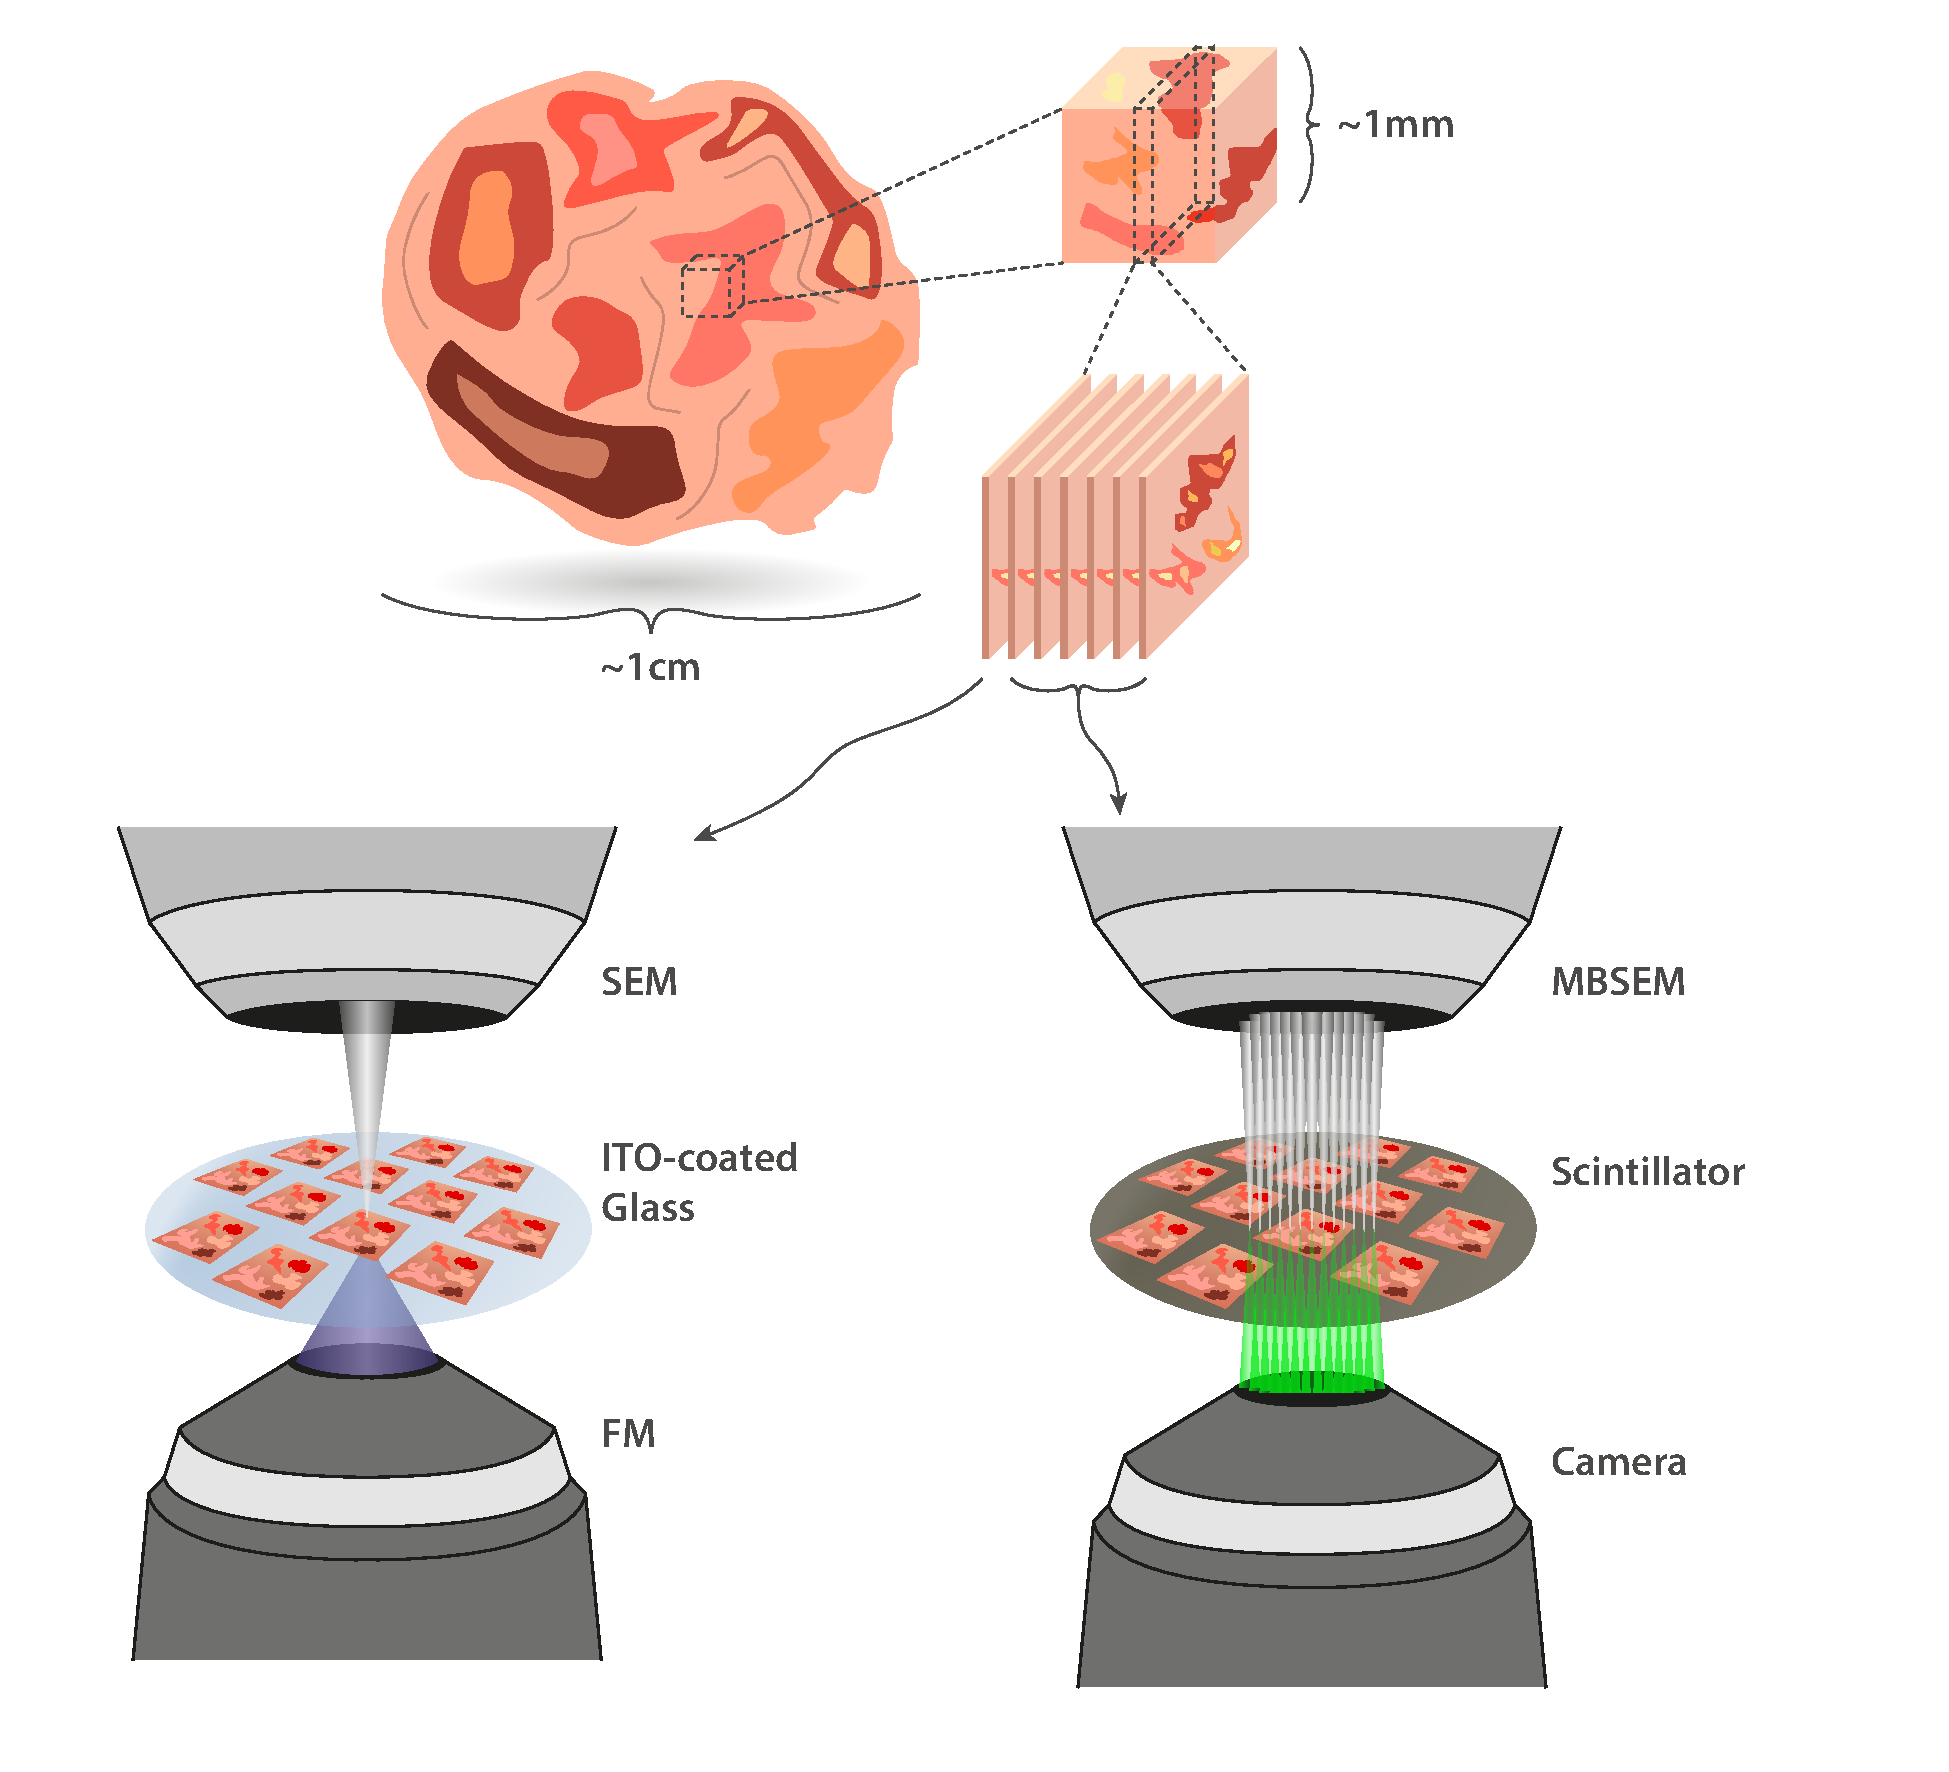
\includegraphics[width=\linewidth]{chapter-5/figures/multibeam_v1.pdf}
    \caption{Prospective workflow for adding artificial fluorescence to multibeam SEM data. Ultrathin sections are prepared for EM with the vast majority placed on a scintillator substrate to be imaged by multibeam SEM, while a small fraction of sections are placed onto ITO-coated glass for integrated CLEM.
    \textbf{TODO: Add neural network stuff? Where does the light from the scintillator actually go? A lens, camera or something else? Clean it up a bit, messy annotations, instruments have different heights, section count probably shouldn't be equal. MBSEM-->FAST-EM and ITO-coated glass --> ITO}}
    \label{fig:5.1_mbsem}
\end{figure}

There are, however, caveats to this approach that must be taken into consideration. First, there is no concrete means of verifying the fluorescence prediction as there is no measured fluorescence to serve as ground truth. Less precise verification methods do exist such as validating the predictions on sections adjacent to those for which the fluorescence was recorded. This may only be reliable, however, for structures significantly larger than the section thickness (e.g. cell nuclei, but not mitochondria, lysosomes, or granules). An alternative approach would be to manually segment the labelled structures in a subset of the FAST-EM data to establish a quasi-ground truth set for assessing the accuracy of the prediction. Another caveat is that there will be sections missing from the FAST-EM imaging volume due to the transfer of sections to ITO-coated glass. However, because the transferred sections will still be imaged with (single beam) SEM, they can be inserted into the image stack for 3D reconstruction, provided they are imaged at the same resolution.

\section{Conclusion}
\label{sec:5.3_conclusion}

We developed a method for 3D CLEM utilizing an integrated light and electron microscope. We began with the realization that conventional SEM imaging of weakly-stained specimen prepared for fluorescence microscopy required highly impractical dwell times. Thus, we implemented a negative bias potential to enhance the backscattered electron (BSE) yield. An empirical optimization of the stage bias, informed by electron optics simulations, ultimately led to orders of magnitude improvement in the signal-to-noise (SNR) ratio. This solved the throughput problem for large-scale, integrated CLEM, which allowed us to develop a scalable workflow for integrated array tomography. The method we created further expedited acquisitions by limiting high-resolution EM to select ROI targeted by fluorescence expression, while high precision EM-FM overlay is achieved using cathodoluminescent markers \cite{haring2017automated}. 

After successfully demonstrating our workflow on pancreatic tissue from different organisms, we explored the potential for large-scale CLEM datasets to be used as training data for machine learning applications. It was found that a modified U-net \cite{ronneberger2015u}, trained on such correlative datasets, was capable of generating high-fidelity predictions of the fluorescence signal from EM. As linking structure to function is one of the primary goals in cell biology, we then tested whether this data would be advantageous in organelle segmentation. While naive approaches of thresholding the measured and predicted fluorescence signals for use as segmentation masks proved unremarkable, more complicated mask generation techniques seem promising. Finally, we discussed the ways in which integrated array tomography could be expanded into a fully automated workflow as well as potential applications for multibeam SEM. Coupling these improvements together with advances in fluorescent probes would bring integrated array tomography to the forefront of volume CLEM, lending new insight to a host of questions within structural biology.



% References
\printbibliography[title={References}]
\end{refsection}
  % conclusion
% \appendix
\chapter{Automatic focusing of the fluorescence microscope}
\label{app:A}

% Customize section counter
\renewcommand\thesection{\Alph{chapter}.\arabic{section}}
\setcounter{section}{0}
\renewcommand{\thefigure}{A.\arabic{figure}}
\setcounter{figure}{0}


% Inputs
% A.1 Problem
% -----------
\section{Original autofocus implementation}
\label{sec:A.1_title}

Acquisition of in-focus fluorescence microscopy (FM) images comprises an essential aspect of the workflow for integrated array tomography. Focusing the objective lens of the fluorescence microscope can be done manually or by an autofocus routine implemented in the microscope control software, Odemis,\footnote{\href{https://github.com/delmic/odemis}{https://github.com/delmic/odemis}} which performs a dichotomic search for optimal focus (Algorithm \ref{alg:odemis_af}). In this routine an image is recorded at the initial position of the objective lens, after which the lens is translated upwards and downwards by a fixed amount. At each position the focus level is measured by the variance of Laplacian (Algorithm \ref{alg:LAPV}). 

\begin{algorithm}
    \caption{Odemis autofocus routine.}
    \label{alg:odemis_af}
    \begin{algorithmic}
        \While {$s \ge s_{min} \textbf{ and } n < n_{max}$}
        \State $M_{mid} \gets \texttt{acquire\_and\_assess}()$
        \State $z \gets +s$ \Comment{Objective is raised}
        \State $M_{up} \gets \texttt{acquire\_and\_assess}()$
        \State $z \gets  -2s$ \Comment{Objective is lowered}
        \State $M_{dwn} \gets \texttt{acquire\_and\_assess}()$
        \If {$M_{up} == M_{dwn}$} \Comment{Minimized step size reached}
            \State \textbf{break}
        \ElsIf {$M_{up} > M_{mid}$}
            \State $z \gets z_0+s$
        \ElsIf {$M_{dwn} > M_{mid}$}
            \State $z \gets z_0-s$
        \Else \Comment{Best focus found at center}
            \State $z \gets z_0$
            \State $s \gets s/2$ \Comment{Reduce step size by half}
        \EndIf
        \State $n \gets n + 1$
        \EndWhile
    \end{algorithmic}
\end{algorithm}


\begin{algorithm}
    \caption{Variance of Laplacian.}
    \label{alg:LAPV}
    \newsavebox\LAP
    \savebox{\LAP}{$\begin{pmatrix} 1/6 & 2/3 & 1/6 \\ 
                                    2/3 & -10/3 & 2/3 \\
                                    1/6 & 2/3 & 1/6 \end{pmatrix}$}
    \begin{algorithmic}
        \State $L \gets $ \usebox{\LAP} \Comment{Laplacian kernel} \\
        \State $I^{*} \gets \texttt{convolve}(I, L)$ \\
        \vspace{0.2em}
        \Return $\texttt{var}(I^{*})$
    \end{algorithmic}
\end{algorithm}

The objective is vertically translated by a given step size in the direction that increases the focus measure until a decrease is observed. The objective is then iteratively raised and lowered by smaller and smaller increments until a minimum change in the focus measure is reached or the algorithm exceeds the maximum number of attempts. While conceptually sound, it was observed that the autofocus routine is susceptible to errors (Figure \ref{fig:A.1_afruns}), even when executed with seemingly favorable initial conditions (i.e. beginning the routine while in focus). The primary issue is thought to originate from an open loop focus actuator, resulting in objective movements with limited precision. This is evidenced by a significant drop in the focus measure for an image acquired as the objective returns to its starting position (Figure \ref{fig:A.1_afruns}, yellow circle). Photobleaching may also play a role in the decrease of the focus measure.

% --- Fig A.1 (AF runs) ---
\begin{figure}[!tb]
    \centering
    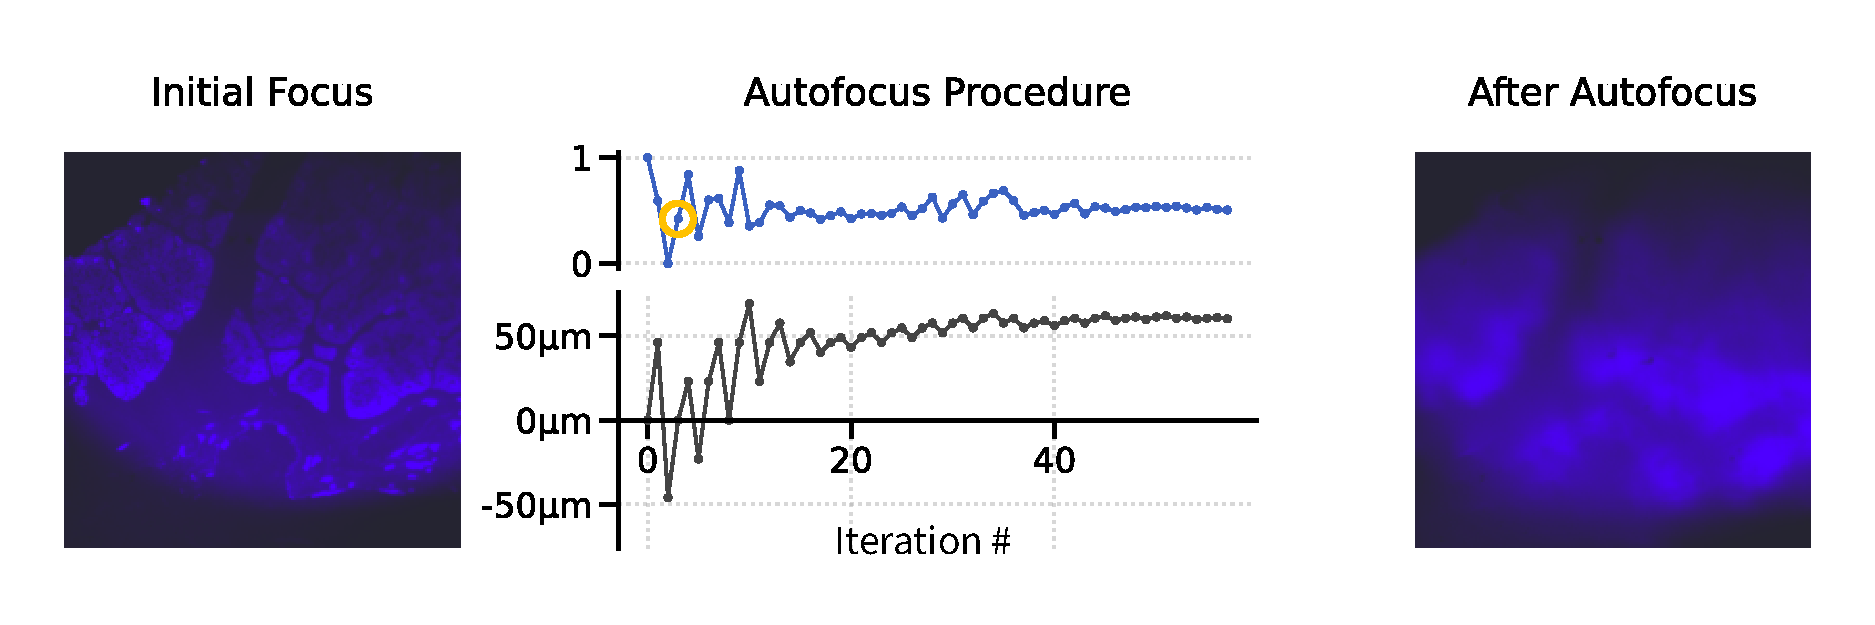
\includegraphics[width=\linewidth]{cppendix-A/figures/figA-1_afruns.pdf}
    \caption{Odemis autofocus routine converging on an out-of-focus image.
    (Left) image from the initial focus position, (center) data from the iterative procedure, (right) image from the final focus position. The two plots show the normalized focus measures (top) and the position of the microscope objective (below) resulting from the dichotomic search. The yellow circle marks the decrease in focus measure when the objective returns to its starting position.}
    \label{fig:A.1_afruns}
\end{figure}


% A.2 Sweeps
% ----------
\section{Analysis of FM focus sweeps}
The results of Figure \ref{fig:A.1_afruns} suggest that a dichotomic search may not be a suitable approach for the autofocus algorithm. Moreover, as will be shown later, Laplacian-based focus measures tend to skew more highly for over-focused images. In order to develop a more robust autofocus algorithm, a series of focus sweeps were conducted over several different $z$ ranges, regions of interest, and fluorescence channels (Figure \ref{fig:A.2_sweeps}). The focus sweeps are analyzed by a selection of different focus metrics (Table \ref{tab:A.1_focus_measures}) compiled from \textcite{pertuz2013analysis}, which examines different focus metrics across a variety of imaging settings and applications. Many of the metrics belong to particular subgroups such as those that involve computing the image gradient (\texttt{GRAE}, \texttt{GRAT}, and \texttt{GRAS}) or the Laplacian (\texttt{LAPE}, \texttt{LAPM}, \texttt{LAPV}, and \texttt{LAPD}). Metrics within each subgroup tend to respond similarly to noise, contrast and window size such that the relative performance depends highly on the particular set of imaging settings \cite{pertuz2013analysis}. The focus metrics were translated from their original Matlab implementation \cite{pertuz2017focus} to Python \cite{Lane_focus-metrics_2022}.

% --- Fig A.2 (sweeps) ---
\begin{figure}[!tb]
    \centering
    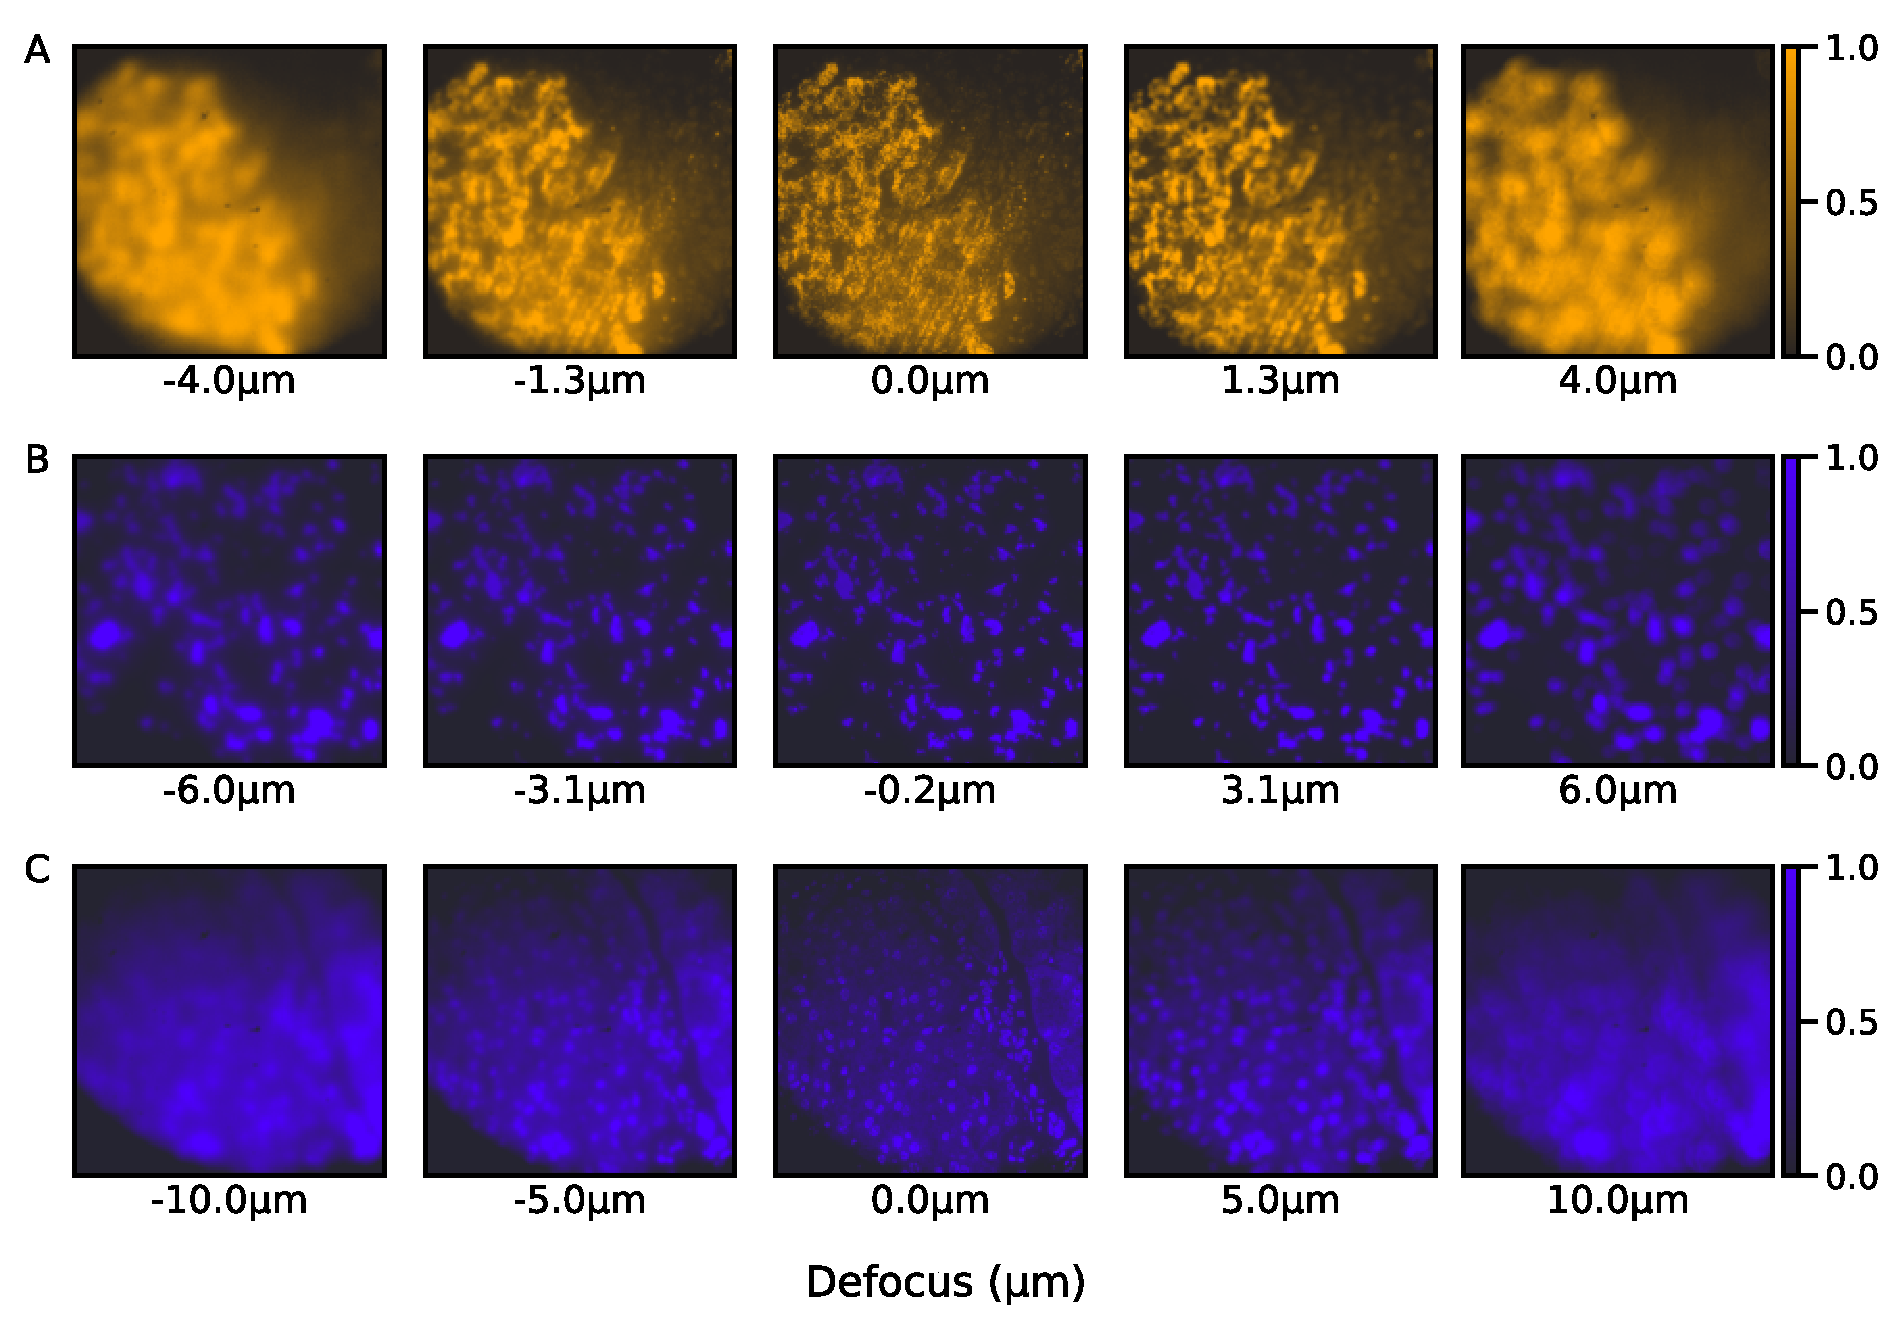
\includegraphics[width=\linewidth]{cppendix-A/figures/figA-2_sweeps.pdf}
    \caption{Sample focus sweeps of the fluorescence microscope.
    (A) An \SI{8}{\micro\meter} sweep over an islet of Langerhans with \SI{555}{\nano\meter} excitation.
    (B) A \SI{12}{\micro\meter} sweep over fluorescent debris on the ITO-coated glass substrate with \SI{405}{\nano\meter} excitation.
    (C) A \SI{20}{\micro\meter} sweep over an islet of Langerhans with \SI{405}{\nano\meter} excitation.}
    \label{fig:A.2_sweeps}
\end{figure}

To assess the relative performance of each focus metric, we perform a consensus analysis to determine how far off each metric is from selecting the correct focus position (Figure \ref{fig:A.3_metrics}). For each focus sweep, the correct focus position is determined by taking the modal value among the 20 focus measures. To better visualize which metrics more frequently return out-of-focus positions, the further away from the modal value a particular curve peaks, the more red that curve appears in the plot. From this analysis it is straightforward to eliminate metrics such as \texttt{ACMO}, \texttt{CURV}, and \texttt{HISE} for which there are multiple red curves. The Laplacian-based metrics can likewise be discarded for their bias towards over-focused images. As expected, there is also a certain degree of redundancy within subgroups. For instance, \texttt{GRAS} (the squared gradient) is virtually equal to \texttt{GRAT} (the thresholded gradient).

% --- Fig A.3 (metrics) ---
\begin{figure}[!tb]
    \centering
    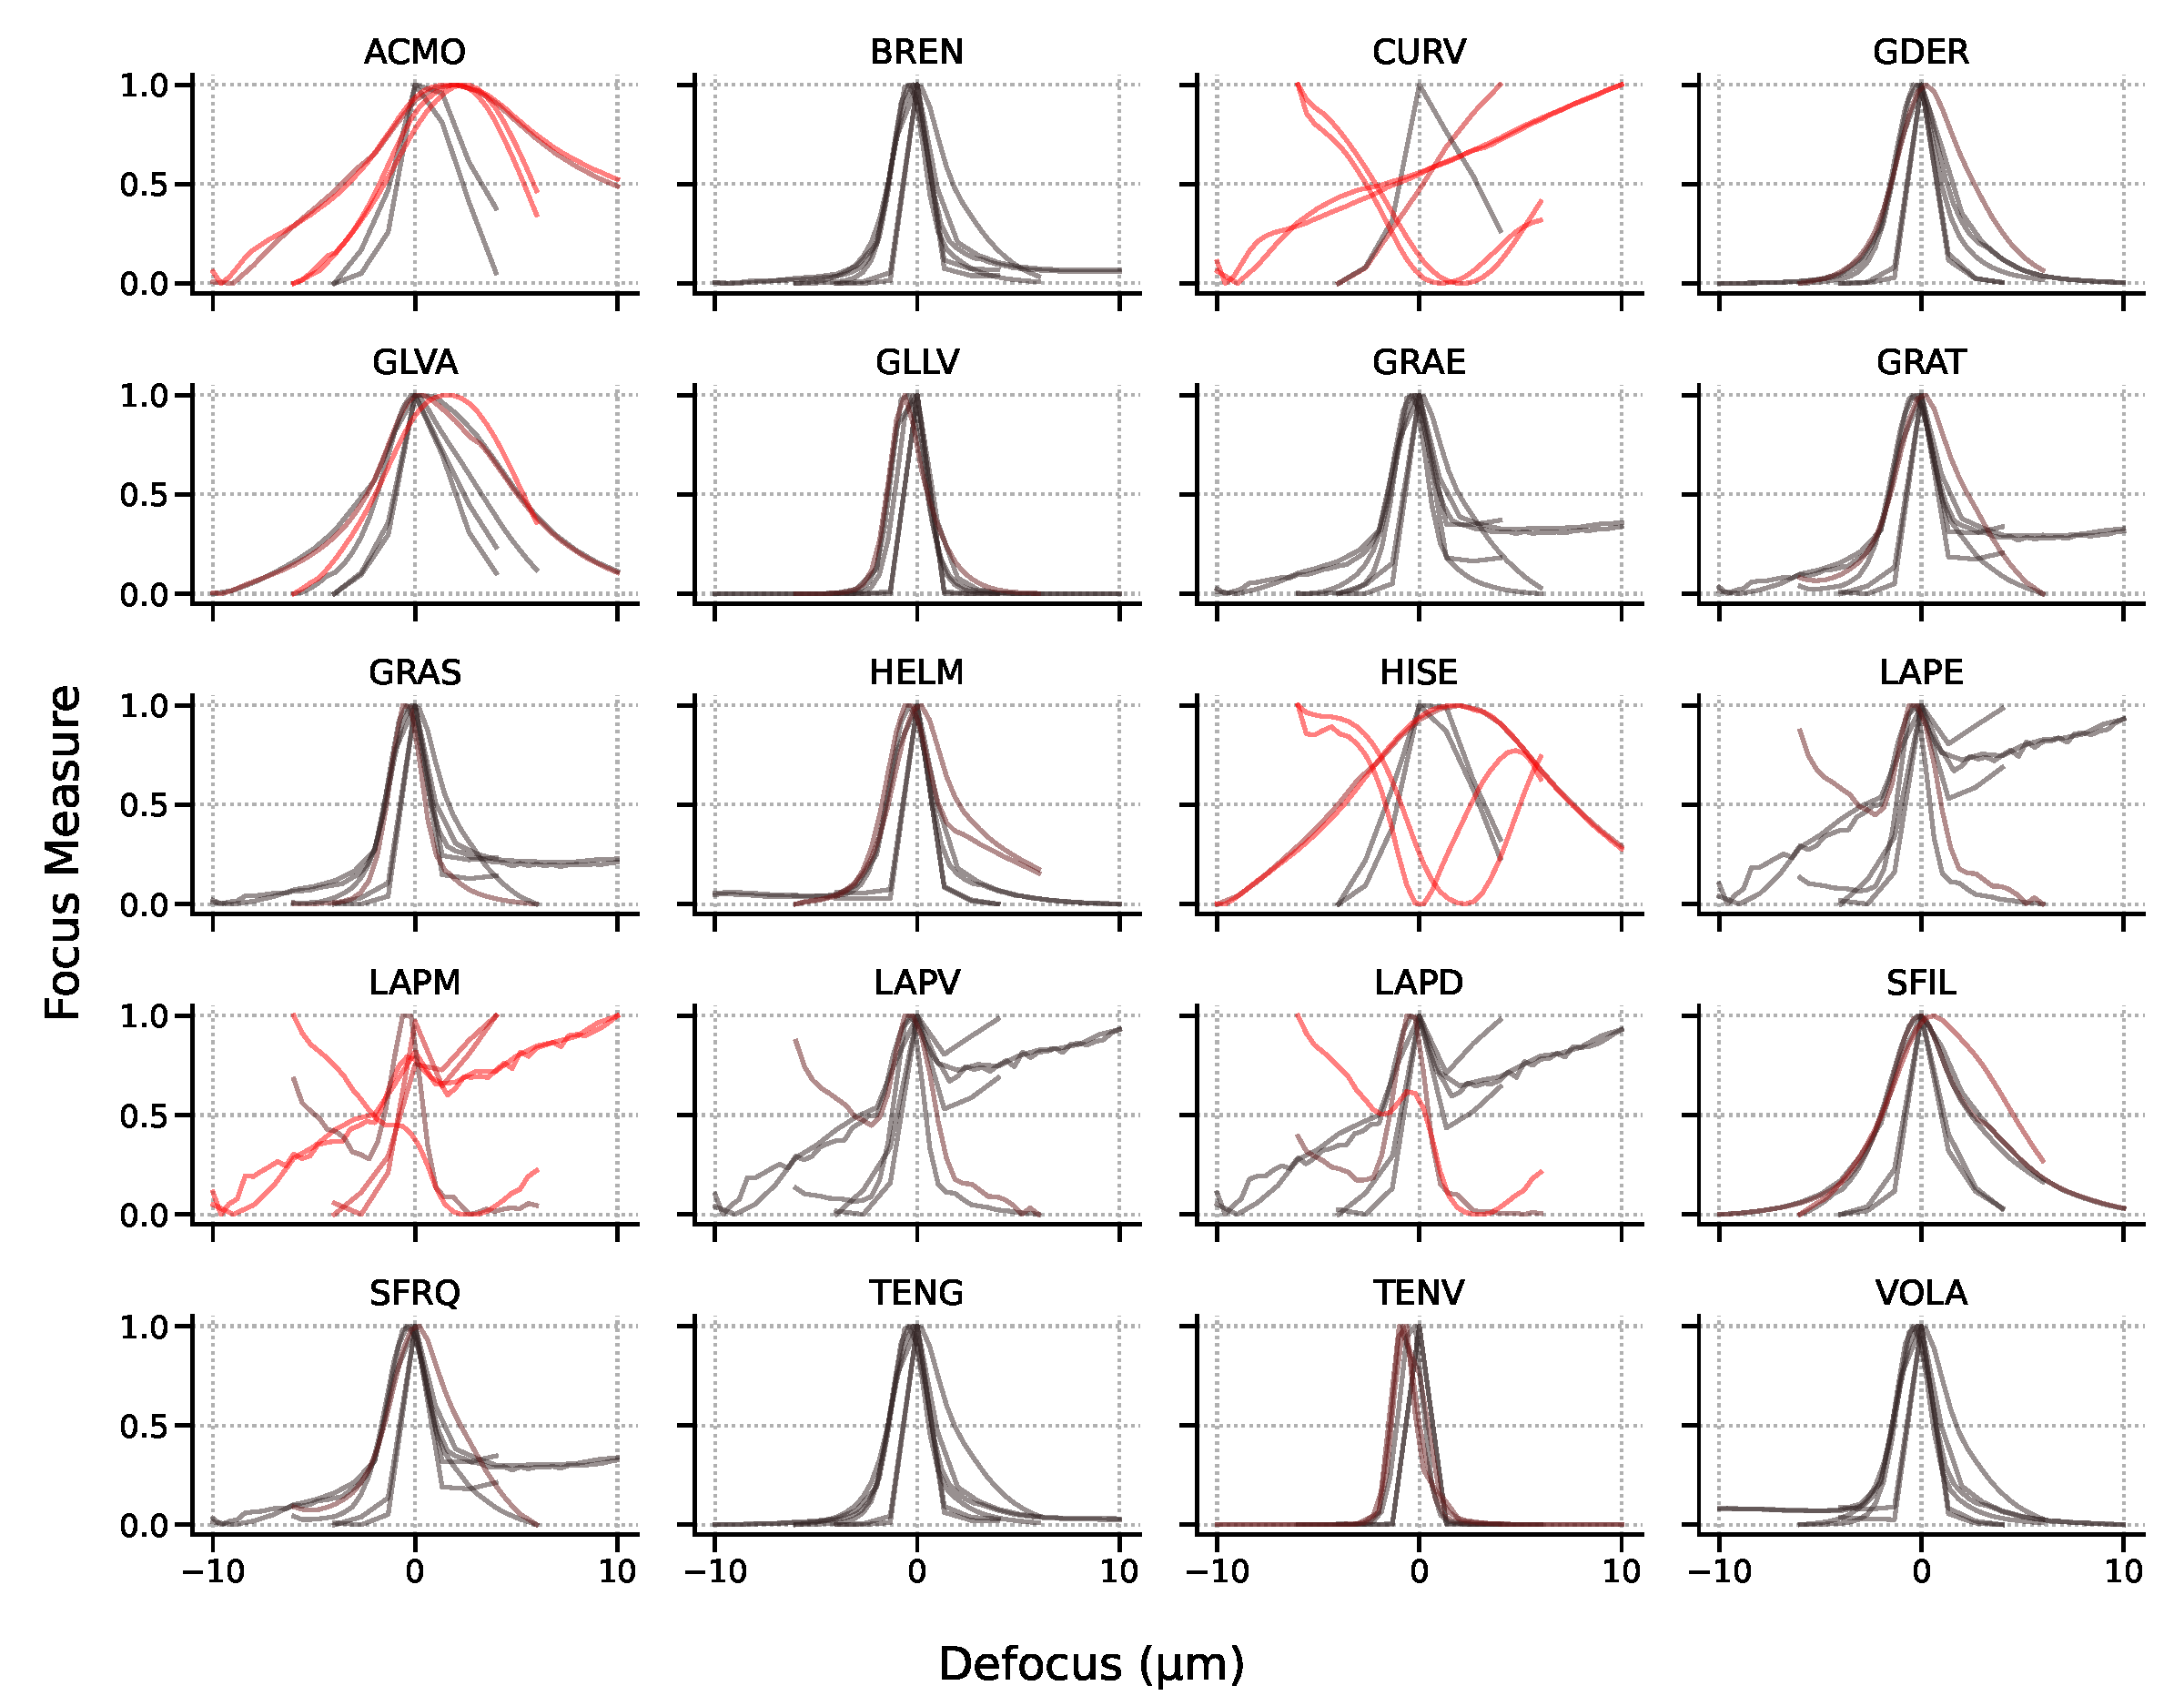
\includegraphics[width=\linewidth]{cppendix-A/figures/figA-3_metrics.pdf}
    \caption{Analysis of 20 potential focus metrics.
    Each subplot shows the focus measures across the six focus sweeps for a particular metric.
    A black color indicates that the peak of the curve is in the consensus (i.e. that the metric returned the correct focus position for that particular sweep).
    Red indicates that the peak of the curve falls outside the consensus, with brighter red signifying that the peak is further away.}
    \label{fig:A.3_metrics}
\end{figure}

After consolidating the candidate focus metrics, we can examine more stringent imaging conditions to explore where the different methods might diverge. To this end, a second round of focus sweeps was recorded in which the images were acquired with decreased exposure times and resolution to present the focus metrics with more challenging settings. The sweeps were then analyzed with the filtered set of candidate focus metrics (Figure \ref{fig:A.4_moresweeps}). The same consensus analysis that was done for the initial set of focus sweeps could not be repeated as the modal value was often erroneous as determined by visual inspection. The correct focus position therefore had to be determined by eye.

% --- Fig A.4 (moresweeps) ---
\begin{figure}[!tb]
    \centering
    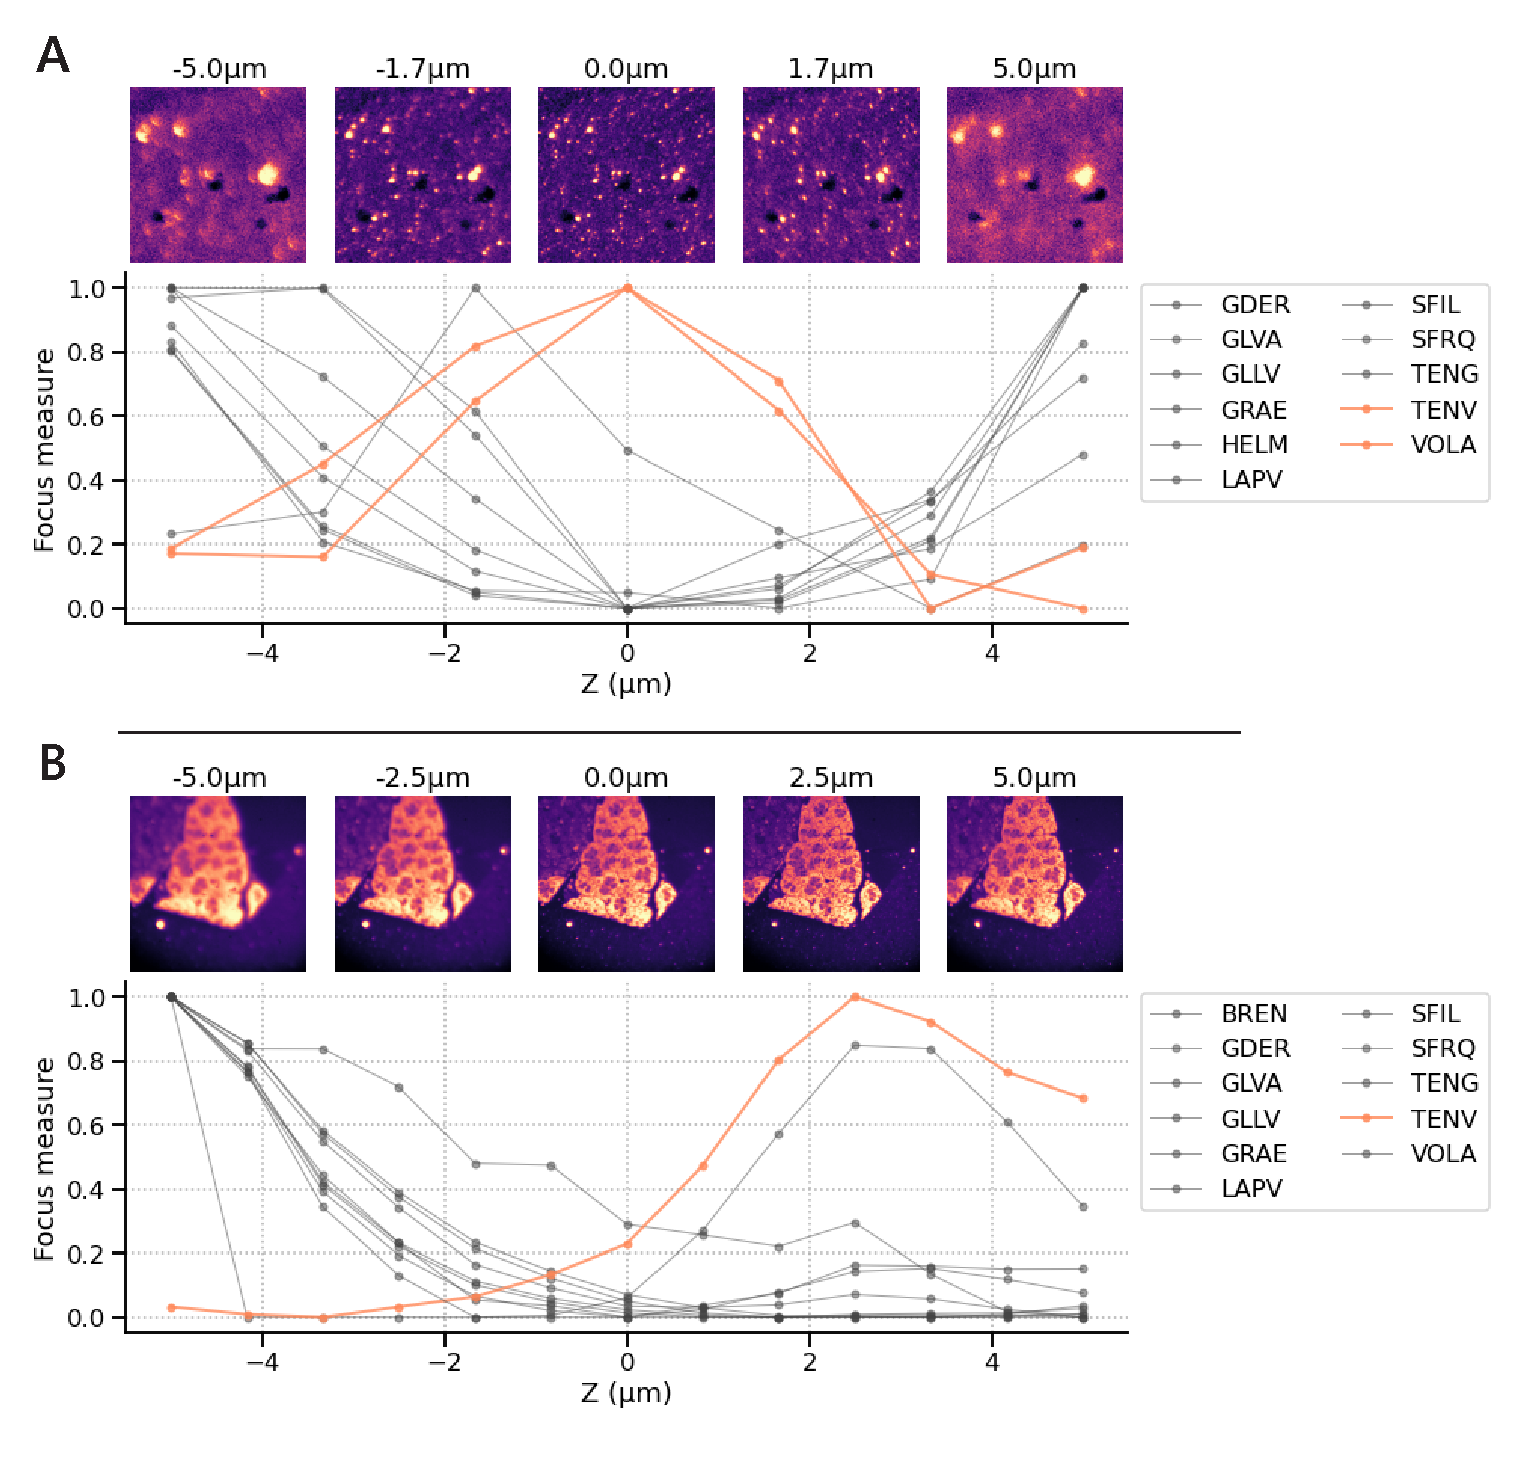
\includegraphics[width=\linewidth]{cppendix-A/figures/figA-4_moresweeps.pdf}
    \caption{Select focus sweeps revealing the robustness of \texttt{TENV} as a focus metric for use with the fluorescence microscope.
    As many of the metrics peaked far from the apparent best focus level, the correct focus position was determined visually.
    (A) A relatively low resolution ($\text{256} \times \text{256}$ \si{\pixel}) focus sweep conducted on the ITO-coated glass background for which only \texttt{TENV} and \texttt{VOLA} yielded the correct focus position.
    (B) A focus sweep acquired on exocrine pancreas tissue with a relatively low exposure time (\SI{100}{\milli\second}) for which only \texttt{TENV} yielded the correct focus position.}
    \label{fig:A.4_moresweeps}
\end{figure}

One metric in particular, \texttt{TENV}, which computes the variance of the image after applying horizontal and vertical Sobel edge detection (Algorithm \ref{alg:TENV}), consistently returned the correct focus position independent of scene, exposure time, and resolution (Figure \ref{fig:A.4_moresweeps}A \& B). A new autofocus routine was therefore developed with \texttt{TENV} as the focus metric and a simple sweep through focus to set the objective position (Algorithm \ref{alg:sweep_af}). To improve precision, the objective position is refined with quadratic interpolation. The new autofocus routine was implemented as an Odemis plugin which could then be integrated into the automated tile acquisitions. Validation was done by automated fluorescence acquisitions on sections of fluorescent HeLa cells embedded in Lowicryl HM20 (Figure \ref{fig:A.5_sections}), resulting in a grid of sharp, well-focused fluorescence images.

% --- Fig A.5 (sections) ---
\begin{figure}[!tb]
    \centering
    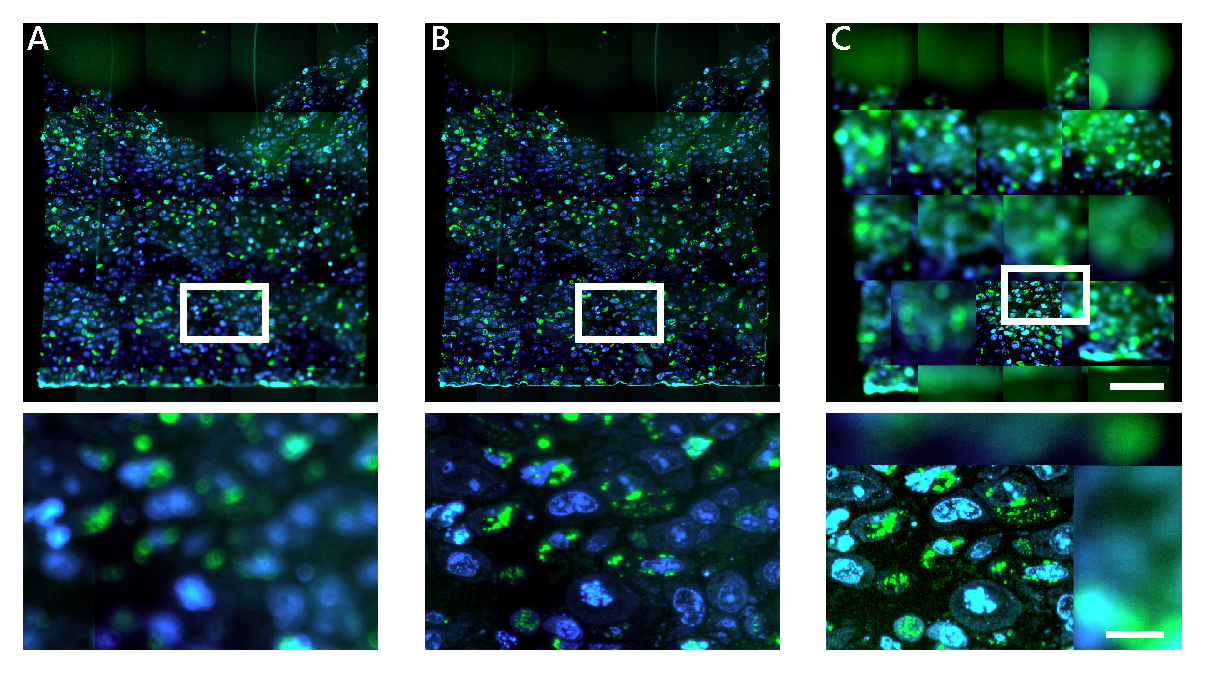
\includegraphics[width=\linewidth]{cppendix-A/figures/figA-5_sections.pdf}
    \caption{Autofocus routine based on focus sweeps and \texttt{TENV} yields best results for automated fluorescence imaging.
    (A) no autofocus routine, (B) the autofocus routine described here, and (C) the default autofocus routine implemented in Odemis.
    All automated fluorescence acquisitions were conducted on the same section of fluorescent HeLa cells.
    Scale bars: (A\,--\,C) \SI{100}{\micro\meter}; (insets) \SI{20}{\micro\meter}.}
    \label{fig:A.5_sections}
\end{figure}


%
\begin{algorithm}
    \caption{Tenengrad variance.}
    \label{alg:TENV}
    \newsavebox\sobelh
    \savebox{\sobelh}{$\begin{pmatrix} 1 &  2 &  1 \\ 
                                       0 &  0 &  0 \\
                                      -1 & -2 & -1 \end{pmatrix}$}
    \newsavebox\sobelv
    \savebox{\sobelv}{$\begin{pmatrix} 1 & 0 & -1 \\ 
                                       2 & 0 & -2 \\
                                       1 & 0 & -1 \end{pmatrix}$}
    \begin{algorithmic}
        \State $S_H \gets $ \usebox{\sobelh} \Comment{Horizontal Sobel filter} \\
        \State $S_V \gets $ \usebox{\sobelv} \Comment{Vertical Sobel filter} \\
        \vspace{0.5em}
        \State $I^{*}_H \gets \texttt{convolve}(I, S_H)$ \\
        \vspace{-1em}
        \State $I^{*}_V \gets \texttt{convolve}(I, S_V)$ \\
        \vspace{0.5em}
        \Return $\texttt{var}\left((I^{*}_H)^2 + (I^{*}_V)^2\right)$
    \end{algorithmic}
\end{algorithm}
%

%
\begin{algorithm}
    \caption{Autofocus algorithm based on sweep through focus.}
    \label{alg:sweep_af}
    \begin{algorithmic}
        \State $M_{max} = 0$
        \State $z \gets -\Delta z/2$
        \For {$i \textbf{ in range } N$}
            \State $M \gets \texttt{acquire\_and\_assess}()$
            \State $M_{max} = \textbf{max}(M, \,M_{max})$
            \State $z \gets +\Delta z/N$
        \EndFor
        \State $z \gets \texttt{QIFFT}([M_{max - 1}, \,M_{max}, \,M_{max + 1}])$ \Comment{Quadratic interpolation}
    \end{algorithmic}
\end{algorithm}
%




 % --- Table A.1 (references) ---
\begin{table}[!tbh]
    \centering
    \caption{Reference list for focus metrics.}
    \label{tab:A.1_focus_measures}
    \begin{tabular}{@{}llr@{}}
    \toprule
    & Focus metric & Reference \\
    \arrayrulecolor{black!30}\midrule
    \texttt{ACMO} & Absolute central moment & \cite{shirvaikar2004optimal} \\
    \texttt{BREN} & Brenner's focus measure & \cite{santos1997evaluation} \\
    \texttt{CURV} & Image curvature & \cite{helmli2001adaptive} \\
    \texttt{GDER} & Gaussian derivative & \cite{geusebroek2000robust} \\
    \texttt{GLVA} & Gray-level variance & \cite{krotkov1986range} \\
    \texttt{GLVV} & Gray-level local variance & \cite{pech2000diatom} \\
    \texttt{GRAE} & Energy of gradient & \cite{subbarao1992focusing} \\
    \texttt{GRAT} & Thresholded gradient & \cite{santos1997evaluation} \\
    \texttt{GRAS} & Squared gradient & \cite{eskicioglu1995image} \\
    \texttt{HELM} & Helmli's measure & \cite{helmli2001adaptive} \\
    \texttt{HISE} & Histogram entropy & \cite{krotkov1986range} \\
    \texttt{LAPE} & Energy of Laplacian & \cite{subbarao1992focusing} \\
    \texttt{LAPM} & Modified Laplacian & \cite{nayar1990shape} \\
    \texttt{LAPV} & Variance of Laplacian & \cite{pech2000diatom} \\
    \texttt{LAPD} & Diagonal Laplacian & \cite{thelen2008improvements}  \\
    \texttt{SFIL} & Steerable filters-based & \cite{minhas20093d} \\
    \texttt{SFRQ} & Spatial frequency & \cite{eskicioglu1995image} \\
    \texttt{TENG} & Tenegrad & \cite{krotkov1986range} \\
    \texttt{TENV} & Tenengrad variance & \cite{pech2000diatom} \\
    \texttt{VOLA} & Vollat's correlation-based & \cite{santos1997evaluation} \\
    \arrayrulecolor{black}\bottomrule
    \end{tabular}
\end{table}


% --- Fig A.6 (timing) ---
\begin{figure}[!tb]
    \centering
    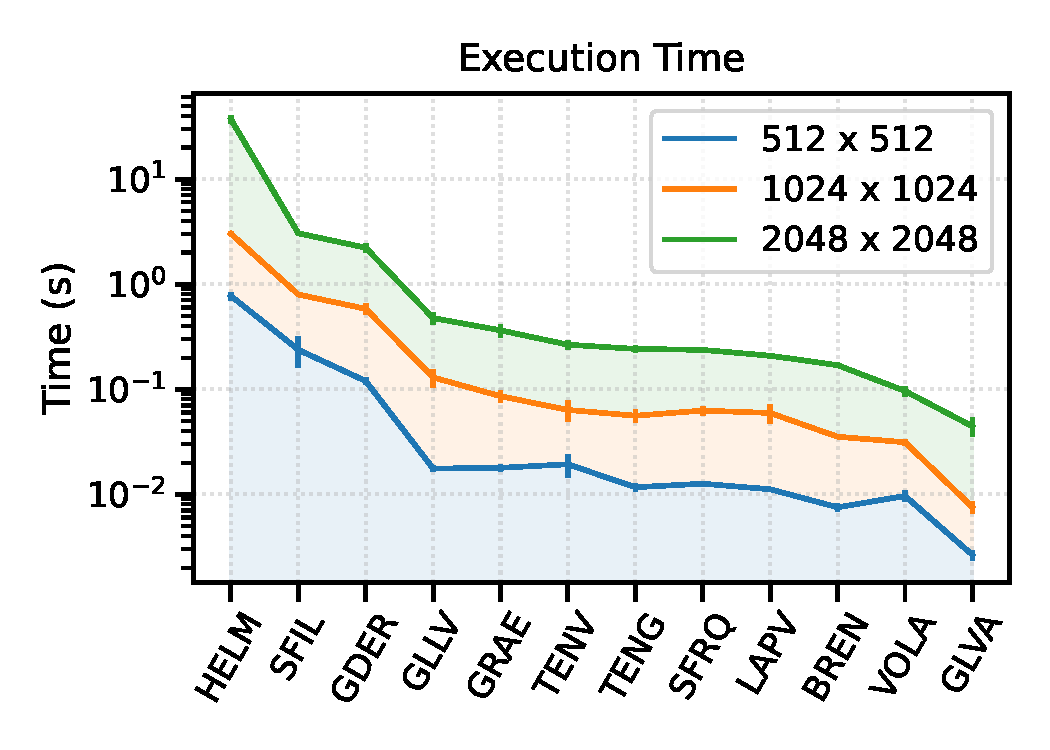
\includegraphics[width=0.7\linewidth]{cppendix-A/figures/figA-6_timing.pdf}
    \caption{Execution times for the filtered set of candidate focus metrics.
    $\text{512}\times\text{512}$, $\text{1024}\times\text{1024}$, and $\text{2048}\times\text{2048}$ denote the image dimensions.}
    \label{fig:A.6_timing}
\end{figure}


% References
\printbibliography[title={References}]
 % FM autofocus


% % For format testing purposes
% \chapter{Test chapter}
\section{Test section}
\blindtext
\subsection{Test subsection}
\blindtext

A new paragraph with a citation \cite{hildebrand2017whole}. Let us also add some numbers with units like \SI{100}{\milli\gram} and even a range of units \SIrange{14}{27}{\kilo\pascal}. \blindtext Could also look at units in math mode like $\SI{13.8}{\newton\per\metre}$. Let's follow this up with some math \cite{delpiano2018automated}.

\blindmathpaper



% TODO:
%   Alternate (short-form) chapter titles
%   Add a splash of color
%   Figure out "parts of this chapter" footnotes
%   Section as appendix at end of each chapter


\end{document}
